\chapter{The Sensitivity of CLIC to Anomalous Gauge Couplings through Vector Boson Scattering}
\label{chap:PhysicsAnalysis}

\chapterquote{Does not wisdom call out? Does not understanding raise her voice?}%
{Proverbs 8:1}

%========================================================================================
%========================================================================================

\section{Motivation}
Vector boson scattering is the interaction of the form $\text{VV} \rightarrow \text{VV}$ where V is any of the electroweak gauge bosons $\text{W}^{+}$, $\text{W}^{-}$, Z or $\gamma$.  This is an interesting process to study because it provides understanding of how the Standard Model Higgs is able to unitarise the otherwise unbounded cross-section for longitudinal massive gauge boson scattering.  Vector boson scattering also provides insights into beyond Standard Model physics that impacts the electroweak sector by probing potential anomalous triple and quartic gauge couplings.  

Triple and quartic gauge couplings lead to interactions of the form $\text{V} \rightarrow \text{VV}$ and $\text{VV} \rightarrow \text{VV}$ respectively.  In the Standard Model there are five allowed vertices, shown in figure \ref{fig:smtripleandquarticvertices}, which arise from the kinematic term $\mathcal{L}_{kin} = -\frac{1}{4}B_{\mu\nu}B^{\mu\nu} - \frac{1}{4}W_{\mu\nu}W^{\mu\nu}$ in the Standard Model Lagrangian.

\begin{figure}[h!]
\subfloat[]{\label{fig:smvertex1}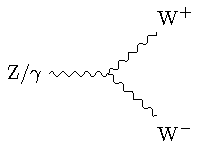
\includegraphics[width=0.3\textwidth]{PhysicsAnalysis/Plots/FeynmanDiagrams/SMVertex1.pdf}} 
\subfloat[]{\label{fig:smvertex2}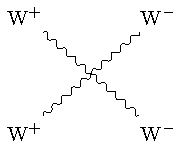
\includegraphics[width=0.3\textwidth]{PhysicsAnalysis/Plots/FeynmanDiagrams/SMVertex2.pdf}} 
\subfloat[]{\label{fig:smvertex3}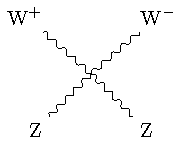
\includegraphics[width=0.3\textwidth]{PhysicsAnalysis/Plots/FeynmanDiagrams/SMVertex3.pdf}} \hfill
\subfloat[]{\label{fig:smvertex4}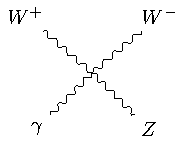
\includegraphics[width=0.3\textwidth]{PhysicsAnalysis/Plots/FeynmanDiagrams/SMVertex4.pdf}} 
\subfloat[]{\label{fig:smvertex5}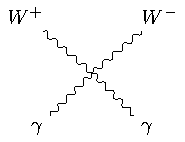
\includegraphics[width=0.3\textwidth]{PhysicsAnalysis/Plots/FeynmanDiagrams/SMVertex5.pdf}} 
\caption[Triple and quartic gauge boson vertices in the Standard Model.]{Triple and quartic gauge boson vertices in the Standard Model.}
\label{fig:smtripleandquarticvertices}
\end{figure}

Anomalous triple and quartic gauge couplings are introduced as parameters in effective field theories (EFTs).  These couplings either modify the Standard Model triple and quartic gauge boson vertices or introduce new triple and quartic vertices that were previously forbidden.  EFTs are a mathematical construct designed to introduce new physics in a manner that builds upon the Standard Model.  They work under the assumption that new physics exists at an energy scale, $\Lambda$, that is much higher than the energy scales currently accessible to modern day particle physics experiments.  In the limit $\Lambda \rightarrow \infty$, the Standard Model is reproduced as the new physics becomes kinematically inaccessible.  Such theories are model independent, giving them a wide span in the search for new physics.  A classic example of an EFT theory is the Fermi theory for beta decay \cite{Fermi:1934hr}.  At energies much below the mass of the W boson, the weak interaction occurring when a neutron decays into a proton, electron and anti-neutrino can be treated as a four-point vertex with quartic coupling strength $\text{G}_{F}$, the Fermi Coupling constant as shown in figure \ref{fig:fermitheory}.

\begin{figure}[h!]
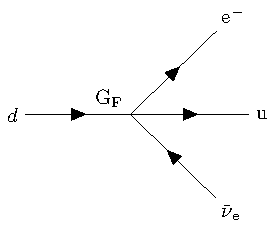
\includegraphics[width=0.5\textwidth]{PhysicsAnalysis/Plots/FeynmanDiagrams/FermiTheory.pdf}
\caption[Four-point vertex proposed for explanation of beta decay by Fermi.]{Four-point vertex proposed for explanation of beta decay by Fermi.} 
\label{fig:fermitheory}
\end{figure}

The study presented in this chapter examines the anomalous quartic gauge couplings $\alpha_{4}$ and $\alpha_{5}$ through vector boson scattering process.  The anomalous gauge couplings that are to be examined are introduced as part of an EFT that is described in chapter \ref{chap:anomalousgaugecouplingtheory}.  The anomalous gauge couplings $\alpha_{4}$ and $\alpha_{5}$ appear in the Lagrangian through the following terms
%
\begin{equation}
\alpha_{4}[\text{Tr}(V^{\mu}V_{\mu})]^{2} \quad \text{ and } \quad \alpha_{5}\text{Tr}(V^{\mu}V_{\nu})] \text{Tr}(V^{\nu}V_{\mu})]\text{ ,}
\end{equation}
%
\noindent where $V_{\mu}$ corresponds, in a carefully chosen gauge, to a linear combination of the massive gauge bosons $\text{W}^{+}$, $\text{W}^{-}$ and Z.  These terms modify the Standard Model vertices $\text{W}^{+}\text{W}^{-} \rightarrow \text{W}^{+}\text{W}^{-}$ and $\text{W}^{+}\text{W}^{-} \rightarrow \text{Z}\text{Z}$ as well as introducing the new vertex $\text{Z}\text{Z} \rightarrow \text{Z}\text{Z}$.  The anomalous gauge couplings $\alpha_{4}$ and $\alpha_{5}$ can be studied in vector boson scattering processes such as those shown in figure \ref{fig:vectorbosonscatteringclic}.  

\begin{figure}[h!]
\subfloat[]{\label{fig:vbsclic1}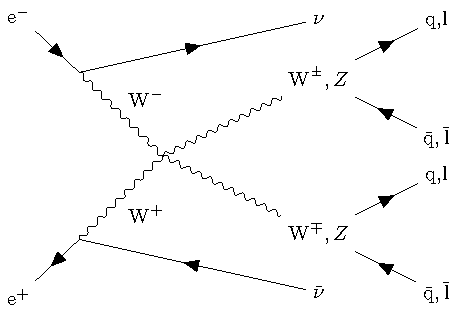
\includegraphics[width=0.5\textwidth]{PhysicsAnalysis/Plots/FeynmanDiagrams/VBSCLIC1.pdf}} \hfill
\subfloat[]{\label{fig:vbsclic2}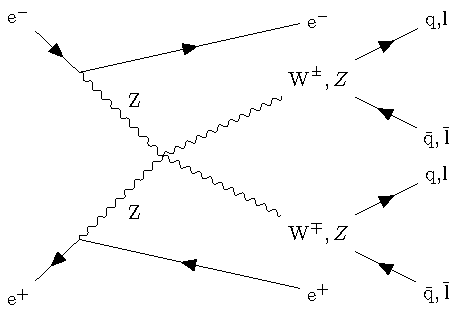
\includegraphics[width=0.5\textwidth]{PhysicsAnalysis/Plots/FeynmanDiagrams/VBSCLIC2.pdf}} \hfill
\subfloat[]{\label{fig:vbsclic3}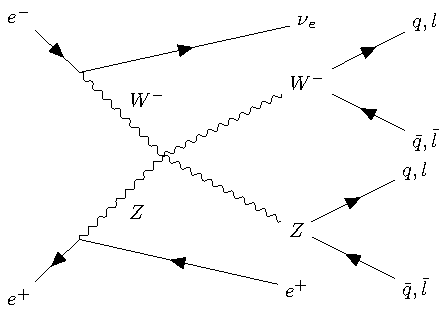
\includegraphics[width=0.5\textwidth]{PhysicsAnalysis/Plots/FeynmanDiagrams/VBSCLIC3.pdf}} \hfill
\subfloat[]{\label{fig:vbsclic4}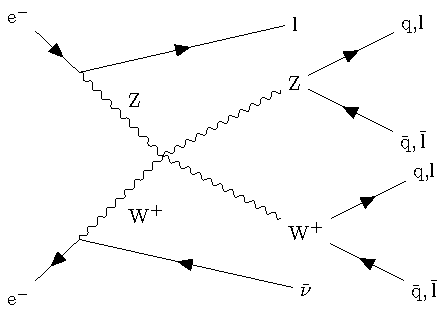
\includegraphics[width=0.5\textwidth]{PhysicsAnalysis/Plots/FeynmanDiagrams/VBSCLIC4.pdf}} \hfill
\caption[Example of vector boson scattering Feynman diagrams showing sensitivity to quartic gauge boson self-interaction vertices.  The processes shown are relevant for CLIC.  In these diagrams q represents the u, d, s, c and b quarks; l represents $\text{e}^{-}$, $\mu^{-}$ and $\tau^{-}$ leptons; and $\nu$ represents the $\nu_{\text{e}}$, $\nu_{\mu}$ and $\nu_{\tau}$ neutrinos.]{Example of vector boson scattering Feynman diagrams showing sensitivity to quartic gauge boson self-interaction vertices.  The processes shown are relevant for CLIC.  In these diagrams q represents the u, d, s, c and b quarks; l represents $\text{e}^{-}$, $\mu^{-}$ and $\tau^{-}$ leptons; and $\nu$ represents the $\nu_{\text{e}}$, $\nu_{\mu}$ and $\nu_{\tau}$ neutrinos.}
\label{fig:vectorbosonscatteringclic}
\end{figure}

CLIC is designed for precision measurements in $\text{e}^{+}\text{e}^{-}$ collisions at high energies and it is ideal for a study of vector boson scattering.  The application of Particle Flow Calorimetry with fine granularity calorimeters gives CLIC excellent jet energy resolution, which allows it to clearly characterise multi-jet final states and final states containing missing energy in the form of neutrinos.  The excellent jet energy resolution also allows for accurate separation of W and Z bosons through di-jet invariant mass, which will be invaluable for event selection.  

The cross-sections for vector boson scattering processes are sufficiently large at the proposed running energies for CLIC to give large signal sample sizes.  A study of anomalous gauge boson couplings at CLIC has the potential to give results several orders of magnitude better than the complementary studies performed at the LHC because of the reduction in hadronic backgrounds and increased cross-section for vector boson scattering processes \cite{Aad:2014zda}.  The above reasons make a strong case for performing a vector boson scattering analysis at CLIC.  

The branching fractions for the hadronic decays of both the $\text{W}^{\pm}$ and Z bosons is of the order of 70\% \cite{Beringer:1900zz}, therefore, the signal final states for the analysis presented in this chapter are vector boson scattering processes where the outgoing bosons decay purely hadronically: $\nu\nu\text{qqqq}$, $\nu\text{lqqqq}$ and llqqqq.  

%========================================================================================
%========================================================================================

\section{Event Generation, Simulation and Reconstruction}
\label{sec:eventgenerationandbackgrounds}
Events were generated using Whizard \cite{0708.4233, hep-ph/0102195} version 1.95.  Due to the presence of beamstrahlung photons in the CLIC beam, events were generated for collisions of $\text{e}^{+}\text{e}^{-}$, $\text{e}^{+}\gamma$, $\gamma\text{e}^{-}$ and $\gamma\gamma$.  The energy spectra used for all particles involved in these collisions took into account the effects of radiation in the form of beamstrahlung photons and the intrinsic energy spread of the CLIC beam.  Furthermore, events involving the interaction between the electromagnetic field of the beam particles involving quasi-real photon mediators with low momenta, described by the Weizsacker-Williams approximation \cite{vonWeizsacker:1934nji, Williams:1935dka} or the Equivalent Photon Approximation (EPA), were generated using Whizard and included in this analysis.  Fragmentation and hadronisation was implemented using PYTHIA 6.4 \cite{Sjostrand:2006za} that was tuned for OPAL $\text{e}^{+}\text{e}^{-}$ collision data recorded at LEP \cite{Alexander:1995bk}.  The decays of tau leptons was simulated using TAUOLA \cite{Was:2000st}.  The full list of events used in this analysis, along with their Standard Model cross-section at $\sqrt{s}=1.4$~TeV can be found in table \ref{table:crosssection1400GeV}.  The samples comprise all final states that are relevant, either as signal or background processes, for an analysis involving the purely hadronic decay channels of the vector boson scattering process:
\begin{itemize}
\item Final states from the purely hadronic decay channels of the vector boson scattering process.  These states are expected to show sensitivity to the anomalous couplings $\alpha_{4}$ and $\alpha_{5}$: $\text{e}^{+}\text{e}^{-} \rightarrow \nu\nu\text{qqqq}$, $\text{e}^{+}\text{e}^{-} \rightarrow \nu\text{lqqqq}$ and $\text{e}^{+}\text{e}^{-} \rightarrow \text{llqqqq}$
\item Final states with four primary quarks arising from $\text{e}^{+}\text{e}^{-}$ interactions: $\text{e}^{+}\text{e}^{-} \rightarrow \text{qqqq}$.
\item Final states with two primary quarks arising from $\text{e}^{+}\text{e}^{-}$ interactions: $\text{e}^{+}\text{e}^{-} \rightarrow \nu{\nu}\text{qq}$, $\text{e}^{+}\text{e}^{-} \rightarrow \nu\text{lqq}$, $\text{e}^{+}\text{e}^{-} \rightarrow \text{llqq}$ and $\text{e}^{+}\text{e}^{-} \rightarrow \text{qq}$.
\item Final states with four primary quarks arising from the interactions of either $\text{e}^{+}$ or $\text{e}^{-}$ with a beamstrahlung photon: $\text{e}^{-}\gamma_{\text{BS}} \rightarrow \text{e}^{-}\text{qqqq}$, $\text{e}^{+}\gamma_{\text{BS}} \rightarrow \text{e}^{+}\text{qqqq}$, $\text{e}^{-}\gamma_{\text{BS}} \rightarrow \nu_{\text{e}}\text{qqqq}$ and $\text{e}^{+}\gamma_{\text{BS}} \rightarrow \overline{\nu}_{\text{e}}\text{qqqq}$.
\item Final states with four primary quarks arising from the interactions of either $\text{e}^{+}$ or $\text{e}^{-}$ with the electromagnetic field of the opposing beam particle.  These cross-sections are calculated using the EPA approximation, which represents the electromagnetic field of the opposing beam particle as a series of photons, so the final states appear as interactions of $\text{e}^{+}$ or $\text{e}^{-}$ with photons: $\text{e}^{-}\gamma_{\text{EPA}} \rightarrow \text{e}^{-}\text{qqqq}$, $\text{e}^{+}\gamma_{\text{EPA}} \rightarrow \text{e}^{+}\text{qqqq}$, $\text{e}^{-}\gamma_{\text{EPA}} \rightarrow \nu_{\text{e}}\text{qqqq}$ and $\text{e}^{+}\gamma_{\text{EPA}} \rightarrow \overline{\nu}_{\text{e}}\text{qqqq}$.
\item Final states with four primary quarks arising from the interaction of the electromagnetic fields of opposing beam particles using the EPA approximation: $\gamma_{\text{EPA}}\gamma_{\text{EPA}} \rightarrow \text{qqqq}$.
\item Final states with four primary quarks arising arising from the interaction of the electromagnetic field of either $\text{e}^{+}$ or $\text{e}^{-}$ using the EPA approximation with a beamstrahlung photon: $\gamma_{\text{EPA}}\gamma_{\text{BS}} \rightarrow \text{qqqq}$ or $\gamma_{\text{BS}}\gamma_{\text{EPA}} \rightarrow \text{qqqq}$.
\item Final states with four primary quarks arising from the interaction of two beamstrahlung photons: $\gamma_{\text{BS}}\gamma_{\text{BS}} \rightarrow \text{qqqq}$.
\end{itemize}
%
\noindent In the above list q represents u, $\bar{\text{u}}$, d, $\bar{\text{d}}$, s, $\bar{\text{s}}$, c, $\bar{\text{c}}$, b or $\bar{\text{b}}$;  l represents $\text{e}^{\pm}$, $\mu^{\pm}$ or $\tau^{\pm}$; and $\nu$ represents $\nu_{\text{e}}$, $\overline{\nu}_{\text{e}}$, $\nu_{\mu}$, $\overline{\nu}_{\mu}$, $\nu_{\tau}$ and $\overline{\nu}_{\tau}$.
%
\begin{table}[h!]
\centering
\begin{tabular}{ l r }
\hline
Final State & Cross-Section [fb] \\ 
\hline
$\text{e}^{+}\text{e}^{-} \rightarrow \nu{\nu}\text{qqqq}$ & 24.7 \\
$\text{e}^{+}\text{e}^{-} \rightarrow \nu\text{lqqqq}$ & 110.4\\
$\text{e}^{+}\text{e}^{-} \rightarrow \text{llqqqq}$ & 62.1\\
$\text{e}^{+}\text{e}^{-} \rightarrow \text{qqqq}$ & 1245.1\\
$\text{e}^{+}\text{e}^{-} \rightarrow \nu{\nu}\text{qq}$ & 787.7\\
$\text{e}^{+}\text{e}^{-} \rightarrow \nu\text{lqq}$ & 4309.7\\
$\text{e}^{+}\text{e}^{-} \rightarrow \text{llqq}$ & 2725.8\\
$\text{e}^{+}\text{e}^{-} \rightarrow \text{qq}$ & 4009.5\\
$\text{e}^{-}\gamma_{\text{EPA}} \rightarrow \text{e}^{-}\text{qqqq}$ & 287.1\\
$\text{e}^{-}\gamma_{\text{BS}} \rightarrow \text{e}^{-}\text{qqqq}$ & 1160.7\\
$\text{e}^{+}\gamma_{\text{EPA}} \rightarrow \text{e}^{+}\text{qqqq}$ & 286.9\\
$\text{e}^{+}\gamma_{\text{BS}} \rightarrow \text{e}^{+}\text{qqqq}$ & 1156.3\\
$\text{e}^{-}\gamma_{\text{EPA}} \rightarrow \nu_{\text{e}}\text{qqqq}$ & 32.6\\
$\text{e}^{-}\gamma_{\text{BS}} \rightarrow \nu_{\text{e}}\text{qqqq}$ & 136.9\\
$\text{e}^{+}\gamma_{\text{EPA}} \rightarrow \overline{\nu}_{\text{e}}\text{qqqq}$ & 32.6\\
$\text{e}^{+}\gamma_{\text{BS}} \rightarrow \overline{\nu}_{\text{e}}\text{qqqq}$ & 136.4\\
$\gamma_{\text{EPA}}\gamma_{\text{EPA}} \rightarrow \text{qqqq}$ & 753.0\\
$\gamma_{\text{EPA}}\gamma_{\text{BS}} \rightarrow \text{qqqq}$ & 4034.8\\
$\gamma_{\text{BS}}\gamma_{\text{EPA}} \rightarrow \text{qqqq}$ & 4018.7\\
$\gamma_{\text{BS}}\gamma_{\text{BS}} \rightarrow \text{qqqq}$ & 21406.2\\
\hline
\end{tabular}
\caption[Cross-sections of signal and background processes at $\sqrt{s}=1.4$~TeV]{Cross-sections of signal and background processes at $\sqrt{s}=1.4$~TeV.  In the above table q represents u, $\bar{\text{u}}$, d, $\bar{\text{d}}$, s, $\bar{\text{s}}$, c, $\bar{\text{c}}$, b or $\bar{\text{b}}$;  l represents $\text{e}^{\pm}$, $\mu^{\pm}$ or $\tau^{\pm}$; and $\nu$ represents $\nu_{\text{e}}$, $\overline{\nu}_{\text{e}}$, $\nu_{\mu}$, $\overline{\nu}_{\mu}$, $\nu_{\tau}$ and $\overline{\nu}_{\tau}$.  The EPA and BS subscript on the incoming photon indicates whether the photon is generated from the equivalent photon approximation or beamstrahlung.}
\label{table:crosssection1400GeV}
\end{table}

Monte-Carlo (MC) samples were simulated using the CLID\_ILD detector model \cite{arXiv:1006.3396}.  Further details of this detector model can be found in chapter \ref{chap:pflowandlcdetectors}.  The simulation was performed in MOKKA \cite{MoradeFreitas:2002kj}, which is a GEANT4 \cite{Agostinelli:2002hh} wrapper providing detailed geometric descriptions of detector concepts for the linear collider.  Events were reconstructed using the MARLIN \cite{Gaede:2006pj} c++ framework, designed for reconstruction at the linear collider.  PandoraPFA \cite{arXiv:0907.3577, arXiv:1209.4039} was used to apply Particle Flow Calorimetry in the reconstruction, the full details of which can be found in chapter \ref{chap:pflowandlcdetectors}.  
  
The effect of the $\gamma\gamma \rightarrow hadrons$ backgrounds, discussed in section \ref{sec:beamrelatedbackgrounds}, were incorporated in the analysis by overlaying $\gamma\gamma \rightarrow hadrons$ events onto the signal and background event samples.  The overlaid backgrounds were added prior to reconstruction so that their impact on the reconstruction was fully accounted for.  For each physics event of interest, $\gamma\gamma \rightarrow hadrons$ background events equivalent to 60 bunch crossings (BXs) are included.  As readout time windows are applied in detector readout, 60 BXs is sufficient for accounting for the $\gamma\gamma \rightarrow hadrons$ backgrounds.  These backgrounds occur in a time window of $-5$~ns to 25~ns around the physics event and the BXs are separated by 0.5~ns, to mimic the CLIC bunch train structure.  The number of background events overlaid per BX is drawn from a Poisson distribution with a mean of 1.3 (3.2) events per bunch crossing at $\sqrt{s}=1.4$~(3)~TeV \cite{Linssen:2012hp}.  

Detector readout is simulated using a readout time window, of 10~ns on all detectors apart from the TPC and HCal barrel.  In the TPC, all hits are retained and in the HCal bareel a 100~ns time window is used to account for the additional time it takes hadronic showers to develop in tungsten \cite{Linssen:2012hp}.  All readout times are corrected for straight time-of-flight to the impact point (IP).  Any hits that have are measured outside of these windows are not used in the reconstruction.   
 
%========================================================================================
%========================================================================================

\section{Modelling of Anomalous Gauge Couplings}
\label{sec:modellingofanomalouscouplings}
The samples that were sensitive to the anomalous gauge couplings $\alpha_{4}$ and $\alpha_{5}$ were generated using Whizard version 1.97, instead of the previously quoted version 1.95.  This change was required as version 1.97 contained a unitarisation scheme that ensured cross-sections for processes involving longitudinal gauge boson scattering did not violate unitarity at the energies considered here.  

Two alternative methods exist for modelling the sensitivity of the vector boson scattering process to the anomalous gauge couplings $\alpha_{4}$ and $\alpha_{5}$.  The first is to generate multiple samples with different values of $\alpha_{4}$ and $\alpha_{5}$ and the second is to generate a single sample with $\alpha_{4} = 0$ and $\alpha_{5} = 0$ and reweight that sample.  The latter approach was taken in this analysis as the former approach is impractical when considering a fine sampling of the $\alpha_{4}$ and $\alpha_{5}$ space.

Event weights, $w$, are calculated according to the ratio of the matrix elements, $M$, for the particular event configuration \cite{WhizardManual}
%
\begin{equation}
w(\alpha_{4},\alpha_{5}) = \frac{|M(event,\alpha_{4},\alpha_{5})|^{2}}{|M(event,0,0)|^{2}} \text{.}
\end{equation}
%
Figure \ref{fig:eventweights1400raw} shows the dependence of the event weights on $\alpha_{4}$ and $\alpha_{5}$ for four individual \nu{\nu}qqqq final state events, generated at $\sqrt{s}=1.4$~TeV.

\begin{figure}[h!]
\centering
\subfloat[]{\label{fig:weight1}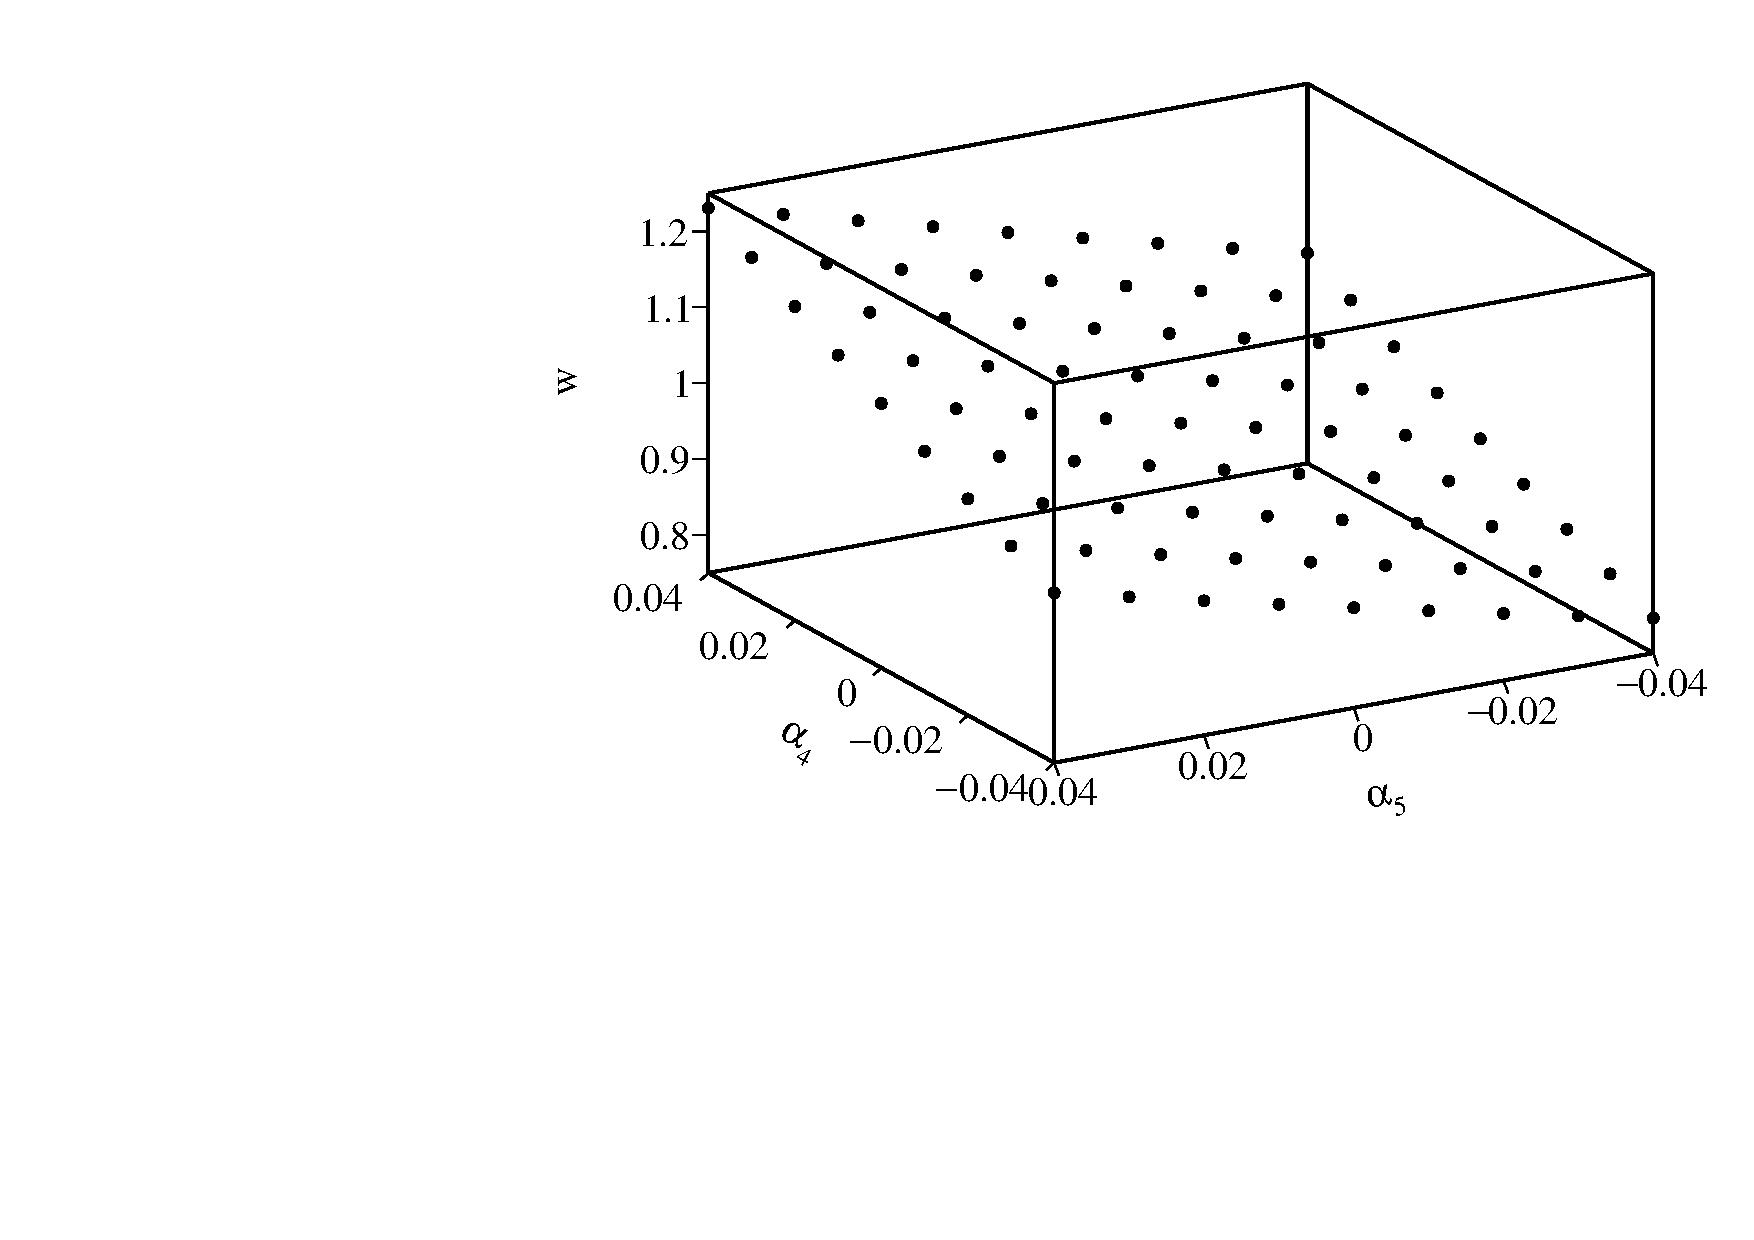
\includegraphics[width=0.5\textwidth]{PhysicsAnalysis/Plots/EventWeights/1400GeV/EventWeightsForEvent100001009_1400GeV_SPFOs_kt_0p70_10Bins_Start_0_End_10_1400GeV_Raw.pdf}}
\subfloat[]{\label{fig:weight2}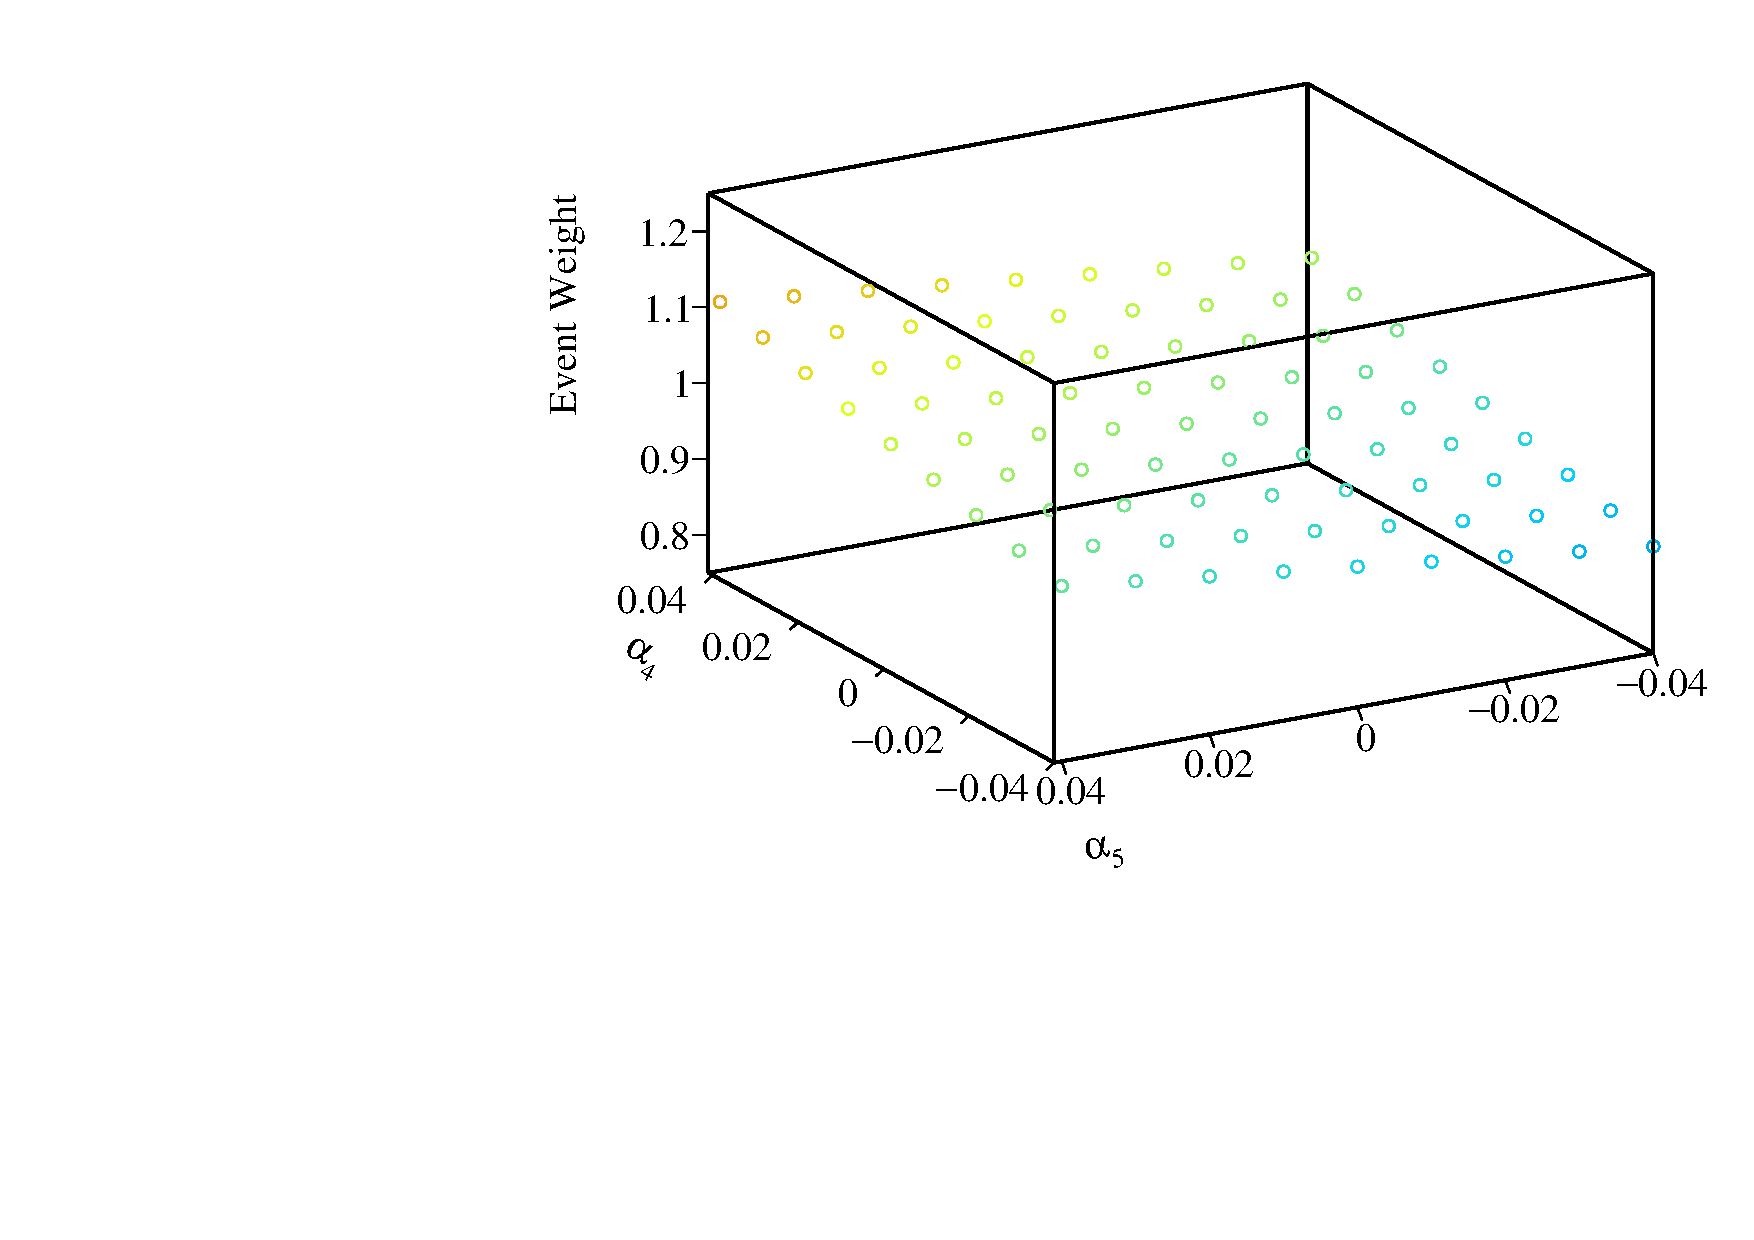
\includegraphics[width=0.5\textwidth]{PhysicsAnalysis/Plots/EventWeights/1400GeV/EventWeightsForEvent100001014_1400GeV_SPFOs_kt_0p70_10Bins_Start_0_End_10_1400GeV_Raw.pdf}} \hfill
\subfloat[]{\label{fig:weight3}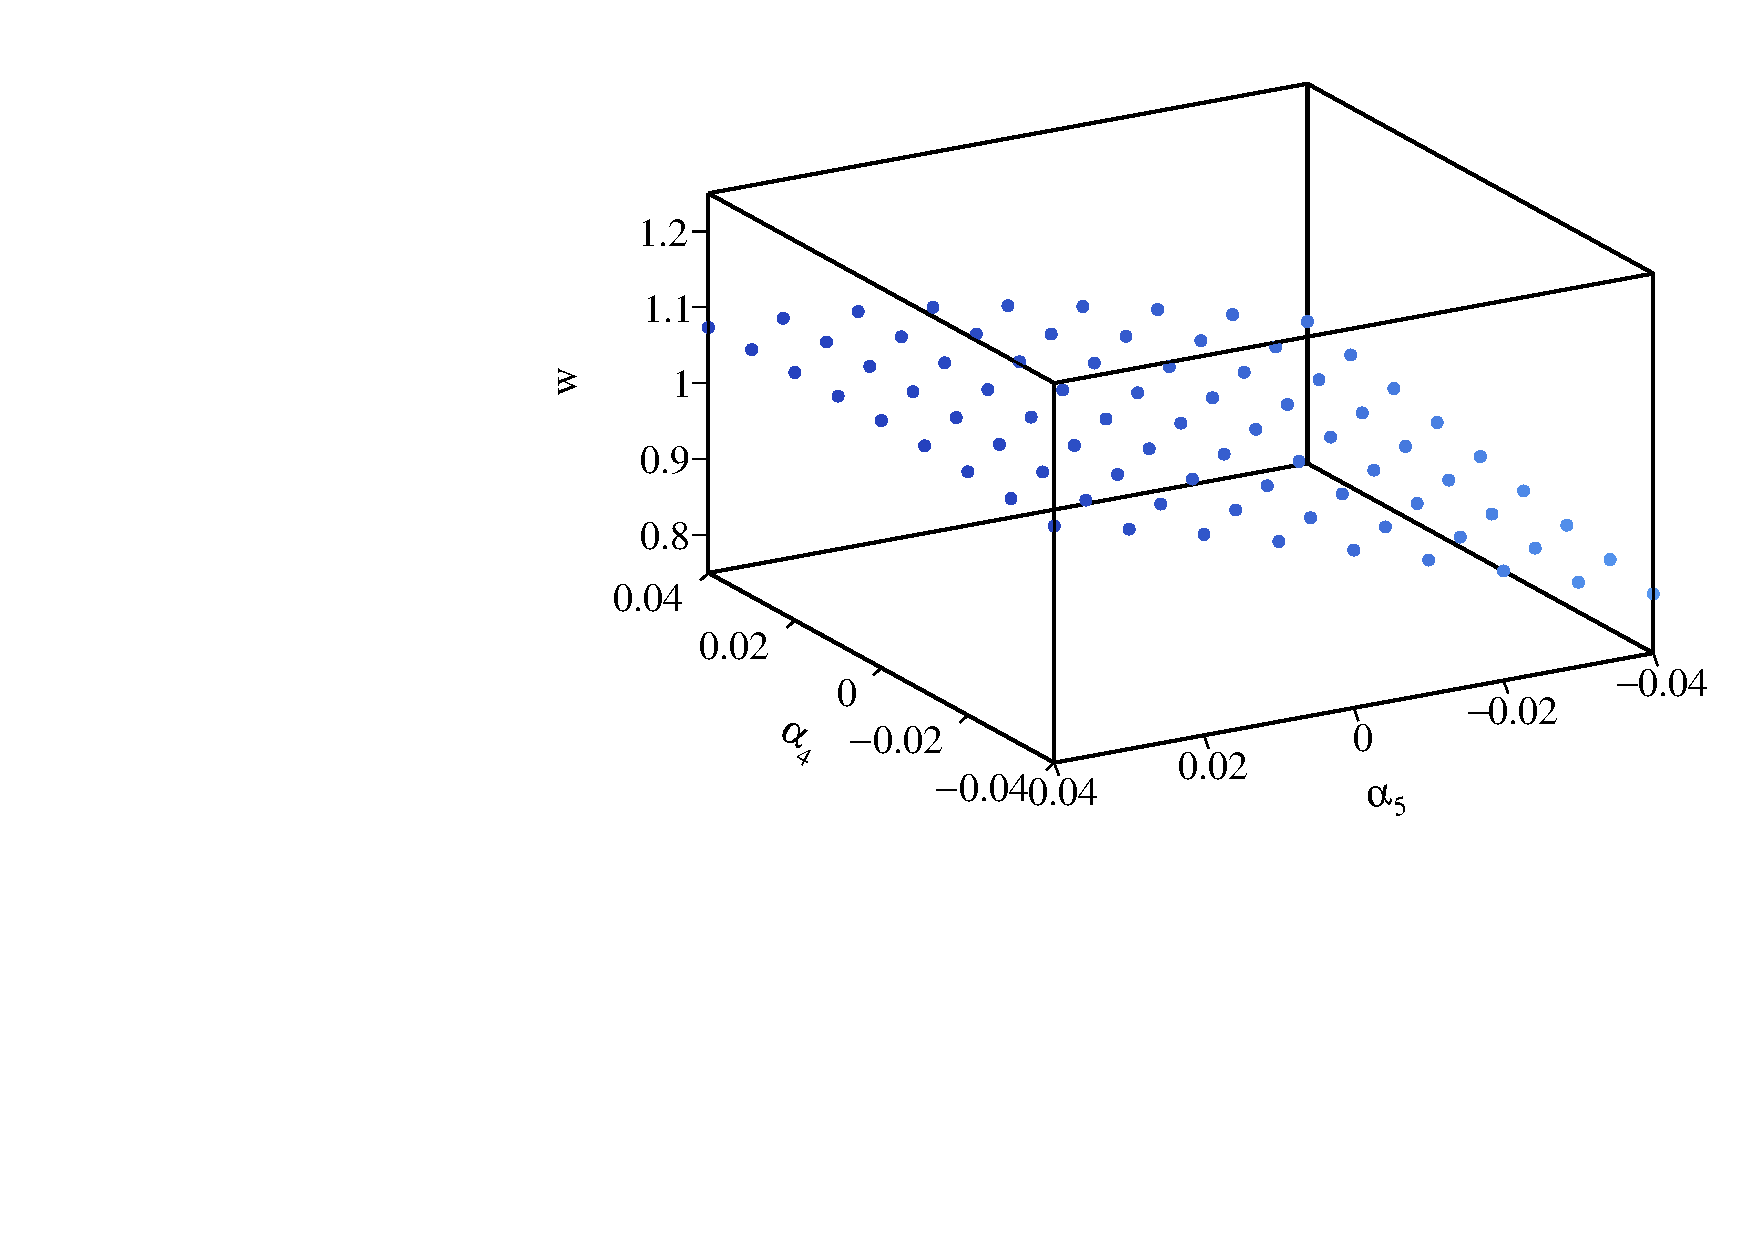
\includegraphics[width=0.5\textwidth]{PhysicsAnalysis/Plots/EventWeights/1400GeV/EventWeightsForEvent100001044_1400GeV_SPFOs_kt_0p70_10Bins_Start_0_End_10_1400GeV_Raw.pdf}}
\subfloat[]{\label{fig:weight4}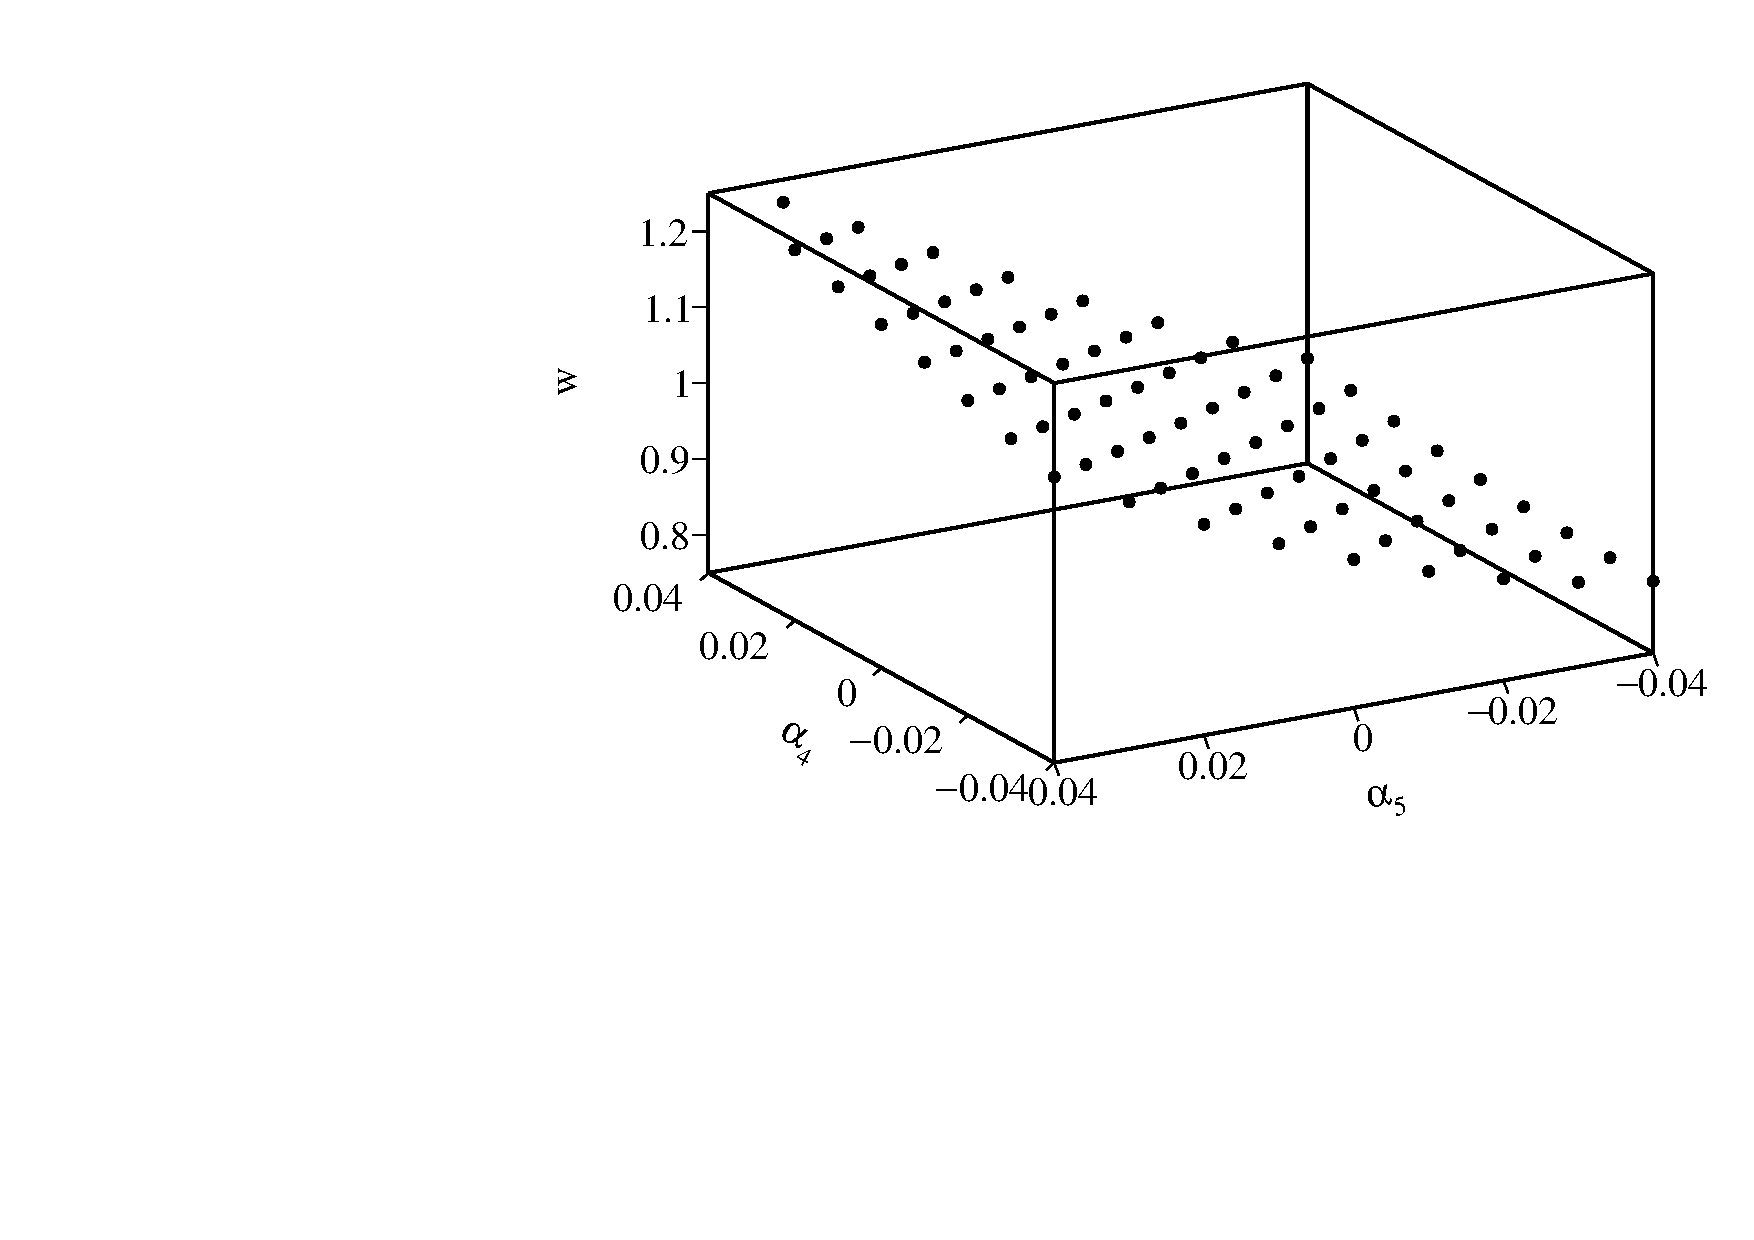
\includegraphics[width=0.5\textwidth]{PhysicsAnalysis/Plots/EventWeights/1400GeV/EventWeightsForEvent100001051_1400GeV_SPFOs_kt_0p70_10Bins_Start_0_End_10_1400GeV_Raw.pdf}}
\caption[The event weights, $w$, determined by the generator as a function of the anomalous couplings $\alpha_{4}$ and $\alpha_{5}$ for a selection of \nu{\nu}qqqq final state events at $\sqrt{s}=1.4$~TeV.]{The event weights, $w$, determined by the generator as a function of the anomalous couplings $\alpha_{4}$ and $\alpha_{5}$ for a selection of \nu{\nu}qqqq final state events at $\sqrt{s}=1.4$~TeV.}
\label{fig:eventweights1400raw}
\end{figure}

Only final states involving contributions from massive gauge boson quartic vertices require reweighting.  Whizard was used to evaluate the cross-sections for all final states shown in table \ref{table:crosssection1400GeV} with $\alpha_{4}=\alpha_{5}=0$ and with $\alpha_{4}=\alpha_{5}=0.05$.  Only the three final states shown in table \ref{table:crosssectionsensitivity1400} were found to have a dependency on $\alpha_{4}$ and $\alpha_{5}$.  

\begin{table}[h!]
\centering
\begin{tabular}{ l r r r r }
\hline
\multirow{ 2}{*}{Final State} & Cross-Section [fb] & Cross-Section [fb] & Percentage \\ 
& ($\alpha_{4} = \alpha_{5} = 0.00$) & ($\alpha_{4} = \alpha_{5} = 0.05$) & Change[\%] \\ 
\hline
$\text{e}^{+}\text{e}^{-} \rightarrow \nu{\nu}\text{qqqq}$ & 24.7 & 34.6 & +40.1 \\
$\text{e}^{+}\text{e}^{-} \rightarrow \nu\text{lqqqq}$ & 115.3 & 113.0 & -2.0 \\
$\text{e}^{+}\text{e}^{-} \rightarrow \text{llqqqq}$ & 62.1 & 68.6 & +10.5 \\
\hline
\end{tabular}
\caption[Cross-sections for selected processes showing the effect of the anomalous gauge couplings $\alpha_{4}$ and $\alpha_{5}$ at $\sqrt{s}=1.4$~TeV.]{Cross-sections for selected processes showing the effect of the anomalous gauge couplings $\alpha_{4}$ and $\alpha_{5}$ at $\sqrt{s}=1.4$~TeV.}
\label{table:crosssectionsensitivity1400}
\end{table}

To maximise the sensitivity to the anomalous gauge couplings, the \nu{\nu}qqqq final state is used to define signal in this analysis.  The {\nu}lqqqq and llqqqq final states are treated as backgrounds that are invariant to changes in $\alpha_{4}$ and $\alpha_{5}$ because they have a much reduced sensitivity to the anomalous gauge couplings in comparison to the \nu{\nu}qqqq final state.  Furthermore, the {\nu}lqqqq and llqqqq final states can be easily vetoed during event selection because of the presence of the primary lepton.  This means the sensitivity of the {\nu}lqqqq and llqqqq final states to the anomalous gauge couplings will have a negligible effect on the results from this study.

Use of the unitarisation scheme in Whizard 1.97, which is needed to ensure cross-sections do not violate unitarity when studying anomalous gauge couplings at CLIC like energies, requires a unit CKM matrix \cite{WhizardManual}.  The impact of this requirement was examined by comparing several reconstructed and MC distributions for \nu{\nu}qqqq final state events generated with Whizard using a Standard Model and unit CKM matrix.  No significant differences were observed, which indicates that enforcing a unit CKM matrix when generating the \nu{\nu}qqqq final state samples did not significantly affect this analysis.  

%========================================================================================
%========================================================================================

\section{Data Analysis}
\label{sec:dataanalysis}
The following section contains a description of how the variables used throughout the anomalous gauge coupling sensitivity study were determined.

%========================================================================================

\subsection{Limiting Beam Related Backgrounds} 
During the reconstruction, after the inner detector tracks have been reconstructed, the CLICTrackSelection processor \cite{arXiv:1209.4039} is applied, which vetoes poorly reconstructed and fake tracks by applying simple quality cuts to the number of hits in the tracking sub-detectors.  The CLICTrackSelection processors also reject tracks where the time of arrival at the calorimeter differs by more than 50~ns between a straight line of flight and a helix fit to the track.  Applying this cut ensures that associations made between charged particles tracks and calorimetric energy deposits are consistent.  

Following the reconstruction, the CLICPfoSelector processor \cite{arXiv:1209.4039} is applied to remove reconstructed particle flow objects (PFOs) that originate from beam related backgrounds.  This processor applies cuts on the $p_{\text{T}}$ and timing information of the PFOs, which vary as a function of position in the detector and the PFO type to target regions of the detector where backgrounds are more prominent, e.g. low $p_{\text{T}}$ for $\gamma\gamma \rightarrow hadrons$ events.  Three configurations of the CLICPfoSelector  have been developed for the CLIC environment and were considered in this analysis.  They are, in order of increasing background rejection, the Loose, Default and Tight selections \cite{arXiv:1209.4039}. 

%========================================================================================

\subsection{Jet Finding} 
\label{sec:jetpairing}
After the application of the CLICPfoSelector, the MarlinFastJet processor, a wrapper for the FastJet \cite{Cacciari:2011ma} processor, was used to cluster each event into four jets.  These jets are then paired up to form two candidate bosons working under the assumption that the correct pairing is achieved when the difference between the invariant masses of the candidate bosons is a minima.  In the case of the signal final state, $\nu\nu$qqqq, it is assumed that the four jets and two candidate bosons map onto the four primary quarks and two outgoing bosons in the vector boson scattering process.  The jet clustering was performed using the longitudinally invariant $k_{t}$ jet algorithm \cite{Catani:1993hr, Ellis:1993tq} in exclusive mode.  The longitudinally invariant $k_{t}$ algorithm proceeds as follows

\begin{enumerate}
\item Determine the $k_{t}$ distance, $d_{ij}$, for each pair of particles, $i$ and $j$, and the beam, $d_{iB}$, distance for each particle, $i$.  These distances are defined as
\begin{equation}
d_{ij} = \text{min}(p_{ti}^{2}, p_{tj}^{2}){\Delta}R^{2}_{ij}/R^{2} \text{ ,} \\
d_{iB} = p_{ti}^{2} \text{ ,}
\end{equation}
where ${\Delta}R^{2}_{ij} = (y_{i} - y_{j})^2 + (\phi_{i} - \phi_{j})^2$, $p_{ti}$ is the transverse momentum of particle $i$, $y_{i}$ is the rapidity of particle $i$, $\phi_{i}$ is the azimuthal angle of the direction of travel of particle $i$ and $R$ is a configurable parameter that typically is of the order of 1.
\item Find the minimum distance, $d_\text{min}$, of all the $k_{t}$ and beam distances.  If the minimum occurs for a $k_{t}$ distance, particles $i$ and $j$ are merged, summing their 4-momenta.  If the beam distance is the minima, particle $i$ was declared to be part of the "beam" jet and the particle is removed from the list of particles and not included in the final jet output.
\item Repeat until the desired number of jets is created.  Alternatively, in inclusive mode this would be repeated until no particles are left in the event.
\end{enumerate}

\noindent Two other clustering algorithms were considered, however, they were found to be inappropriate for the experimental conditions at CLIC.  These alternative algorithm choices are applied in the same manner as the longitudinally invariant $k_{t}$ algorithm, however, they differ in the definition of $d_{ij}$ and $d_{iB}$.  Figure \ref{fig:invariantmassalgoveto} shows the distribution of the invariant mass of the candidate bosons at $\sqrt{s}=1.4$~TeV \nu{\nu}qqqq final state events for each of the jet algorithms considered.  The candidate boson masses are determined by forcing the events into 4 jets and then pairing the jet pairs to form candidate bosons.  The jet pairing configuration is determined by pairing jets such that the mass differences between the two candidate bosons is a minimum.  

\begin{figure}[h!]
\centering
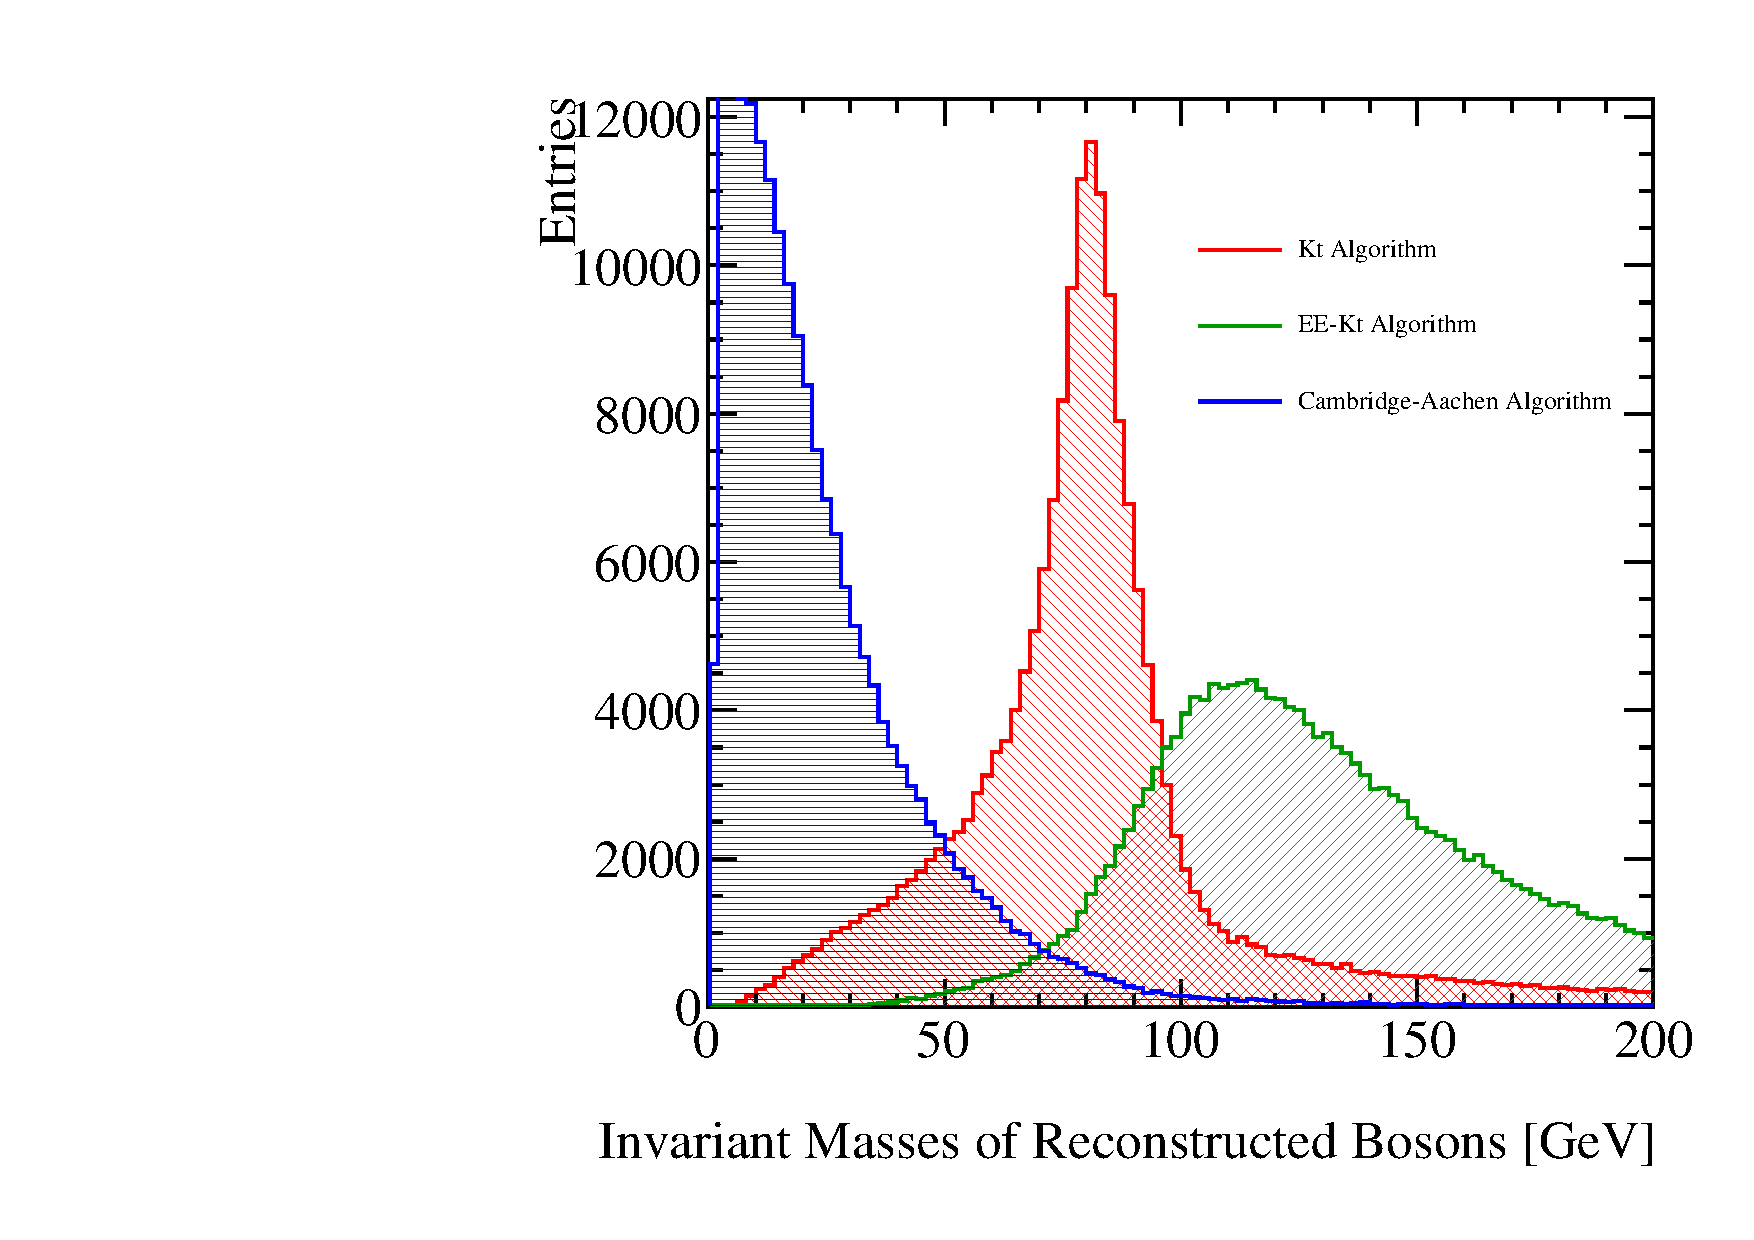
\includegraphics[width=0.5\textwidth]{PhysicsAnalysis/Plots/SimpleInvMassPlot/InvariantMassesAlgorithmVeto.pdf}
\caption[The reconstructed masses for different choices of jet algorithm at $\sqrt{s}=1.4$~TeV \nu{\nu}qqqq final state events.  These samples should be dominated by vector boson scattering involving pairs of outgoing W bosons and so it is expected that a peak at the W boson mass, $m_{W} = 80.385 \pm 0.015$~GeV \cite{Beringer:1900zz}, should be observed.  In the case of the $k_{t}$ algorithm and the $\text{e}^{+}\text{e}^{-}k_{t}$  algorithm an R parameter of 0.7 was used.  All distributions show raw number of events.]{The reconstructed masses for different choices of jet algorithm at $\sqrt{s}=1.4$~TeV \nu{\nu}qqqq final state events.  These samples should be dominated by vector boson scattering involving pairs of outgoing W bosons and so it is expected that a peak at the W boson mass, $m_{W} = 80.385 \pm 0.015$~GeV \cite{Beringer:1900zz}, should be observed.  In the case of the $k_{t}$ algorithm and the $\text{e}^{+}\text{e}^{-}k_{t}$  algorithm an R parameter of 0.7 was used.  All distributions show raw number of events.}
\label{fig:invariantmassalgoveto}
\end{figure}

The first alternative jet algorithm considered was the $k_{t}$ algorithm for $\text{e}^{+}\text{e}^{-}$ colliders \cite{Catani:1991hj}, the $\text{e}^{+}\text{e}^{-}k_{t}$  or Durham algorithm.  In this algorithm $d_{iB}$ is not used and 
%
\begin{equation}
d_{ij} = 2\text{min}(E_{i}^{2}, E_{j}^{2})(1-cos\theta_{ij}) \text{ ,}
\end{equation}
%
\noindent where $\theta_{ij}$ is the opening angle of particles $i$ and $j$ and $E_{i}$ is the energy of particle $i$.  In the collinear limit $d_{ij}$ corresponds to the relative transverse momenta of the particles.  The major failure of this algorithm when applied to CLIC is the absence of $d_{iB}$, which leads to large numbers of beam related background particles being associated to jets.  As figure \ref{fig:invariantmassalgoveto} shows, the invariant mass of the paired jets, which should peak around the W and Z boson masses, is much larger than expected, due to the presence of these backgrounds.  Also this algorithm is not invariant to boosts along the beam direction meaning that it is inappropriate for use at CLIC given the beam induced backgrounds modify the nominal collision kinematics.  

The second alternative jet algorithm considered was the Cambridge-Aachen jet algorithm \cite{Dokshitzer:1997in} where 
%
\begin{equation}
d_{ij} = {\Delta}R_{ij}^{2}/R^2 \text{ ,} \\
d_{iB} = 1 \text{ .}
\end{equation}
%
\noindent This algorithm performs poorly as it does not account for the transverse momentum or the energy of the particles being clustered. In essence, this is a cone clustering algorithm with a cone radius defined through ${\Delta}R_{ij} = R$, which even for large R was found to discard too much energy in the event to be useful for this analysis.  This can be seen in figure \ref{fig:invariantmassalgoveto} where the invariant mass of the paired jets is much lower than expected.  This algorithm is appropriate for events that contain highly boosted jets, however, at CLIC the jets are too disperse for this algorithm to be successful.

%========================================================================================

\subsubsection{Optimal Jet Finding Algorithm}
\label{sec:optimaljetalgorithm}
Optimisation of the jet finding procedure was performed on both the PFO selection and the value of the R parameter used in the longitudinally invariant $k_{t}$ algorithm.  The optimisation procedure involved performing the sensitivity study, described in section \ref{sec:fitting}, using solely the {\nu}{\nu}qqqq signal final state.  This methodology ensures that the optimisation was done with respect to the physics of interest without having to perform the jet reconstruction for the large number of background events for each jet algorithm configuration considered. 

Table \ref{table:precisionsignaljetalgo1400GeV} shows the 68\% confidence limits on the measurement of $\alpha_{4}$ and $\alpha_{5}$ obtained using the {\nu}{\nu}qqqq signal final state only at $\sqrt{s} = 1.4$~TeV for different jet algorithm configurations.  These confidence limits represent the idealised sensitivity of the CLIC experiment to the anomalous gauge couplings.  Once the effects of backgrounds and event selection are included in the analysis, these confidence limits will increase in size.

\begin{table}[h!]
\centering
\begin{tabular}{l c c c}
\hline
& \multicolumn{3}{c}{PFO Selection} \\ 
R Parameter & Tight Selected PFOs & Selected PFOs & Loose Selected PFOs \\ 
\hline
\multirow{ 2}{*}{0.7} & $-0.0039 < \alpha_{4} < 0.0051$ & $-0.0035 < \alpha_{4} < 0.0047$ & $-0.0037 < \alpha_{4} < 0.0047$ \\
                                & $-0.0027 < \alpha_{5} < 0.0031$ & $-0.0025 < \alpha_{5} < 0.0031$ & $-0.0024 < \alpha_{5} < 0.0028$ \\
\hline
\multirow{ 2}{*}{0.9} & $-0.0036 < \alpha_{4} < 0.0047$ & $-0.0035 < \alpha_{4} < 0.0045$ & $-0.0035 < \alpha_{4} < 0.0045$ \\
                                & $-0.0026 < \alpha_{5} < 0.0031$ & $-0.0023 < \alpha_{5} < 0.0027$ & $-0.0022 < \alpha_{5} < 0.0027$ \\
\hline
\multirow{ 2}{*}{1.1} & $-0.0036 < \alpha_{4} < 0.0047$ & $-0.0036 < \alpha_{4} < 0.0048$ & $-0.0036 < \alpha_{4} < 0.0046$ \\
                                & $-0.0026 < \alpha_{5} < 0.0031$ & $-0.0025 < \alpha_{5} < 0.0029$ & $-0.0024 < \alpha_{5} < 0.0028$ \\
\hline
\end{tabular}
\caption[The 68\% confidence limits on the measurement of $\alpha_{4}$ and $\alpha_{5}$ obtained using the {\nu}{\nu}qqqq signal final state only at $\sqrt{s} = 1.4$~TeV for different jet algorithm configurations.]{The 68\% confidence limits on the measurement of $\alpha_{4}$ and $\alpha_{5}$ obtained using the {\nu}{\nu}qqqq signal final state only at $\sqrt{s} = 1.4$~TeV for different jet algorithm configurations.}
\label{table:precisionsignaljetalgo1400GeV}
\end{table}

The configuration for the jet algorithm for the $\sqrt{s}=1.4$~TeV analysis was chosen as selected PFOs with an R parameter of 0.9.  While the loose PFO selection gives a marginally better performance, the selected PFO selection was preferred to minimise the effect of the $\gamma\gamma \rightarrow hadrons$ background.  Figure \ref{fig:chi2jetalgoideal1400GeV} shows confidence contours, given a null hypothesis of $\alpha_{4} = \alpha_{5} = 0$, for the selected PFO and R parameter of 0.9 jet algorithm configuration at $\sqrt{s}=1.4$~TeV.  Figures \ref{fig:a4chi2jetalgoideal1400GeV} and \ref{fig:a5chi2jetalgoideal1400GeV} show the one dimensional $\chi^{2}$ distribution for $\alpha_{4}$ and $\alpha_{5}$, assuming $\alpha_{5} = 0$ and $\alpha_{4} = 0$ respectively, for the same configuration.  

\begin{figure}[h!]
\centering
\subfloat[]{\label{fig:chi2jetalgoideal1400GeV}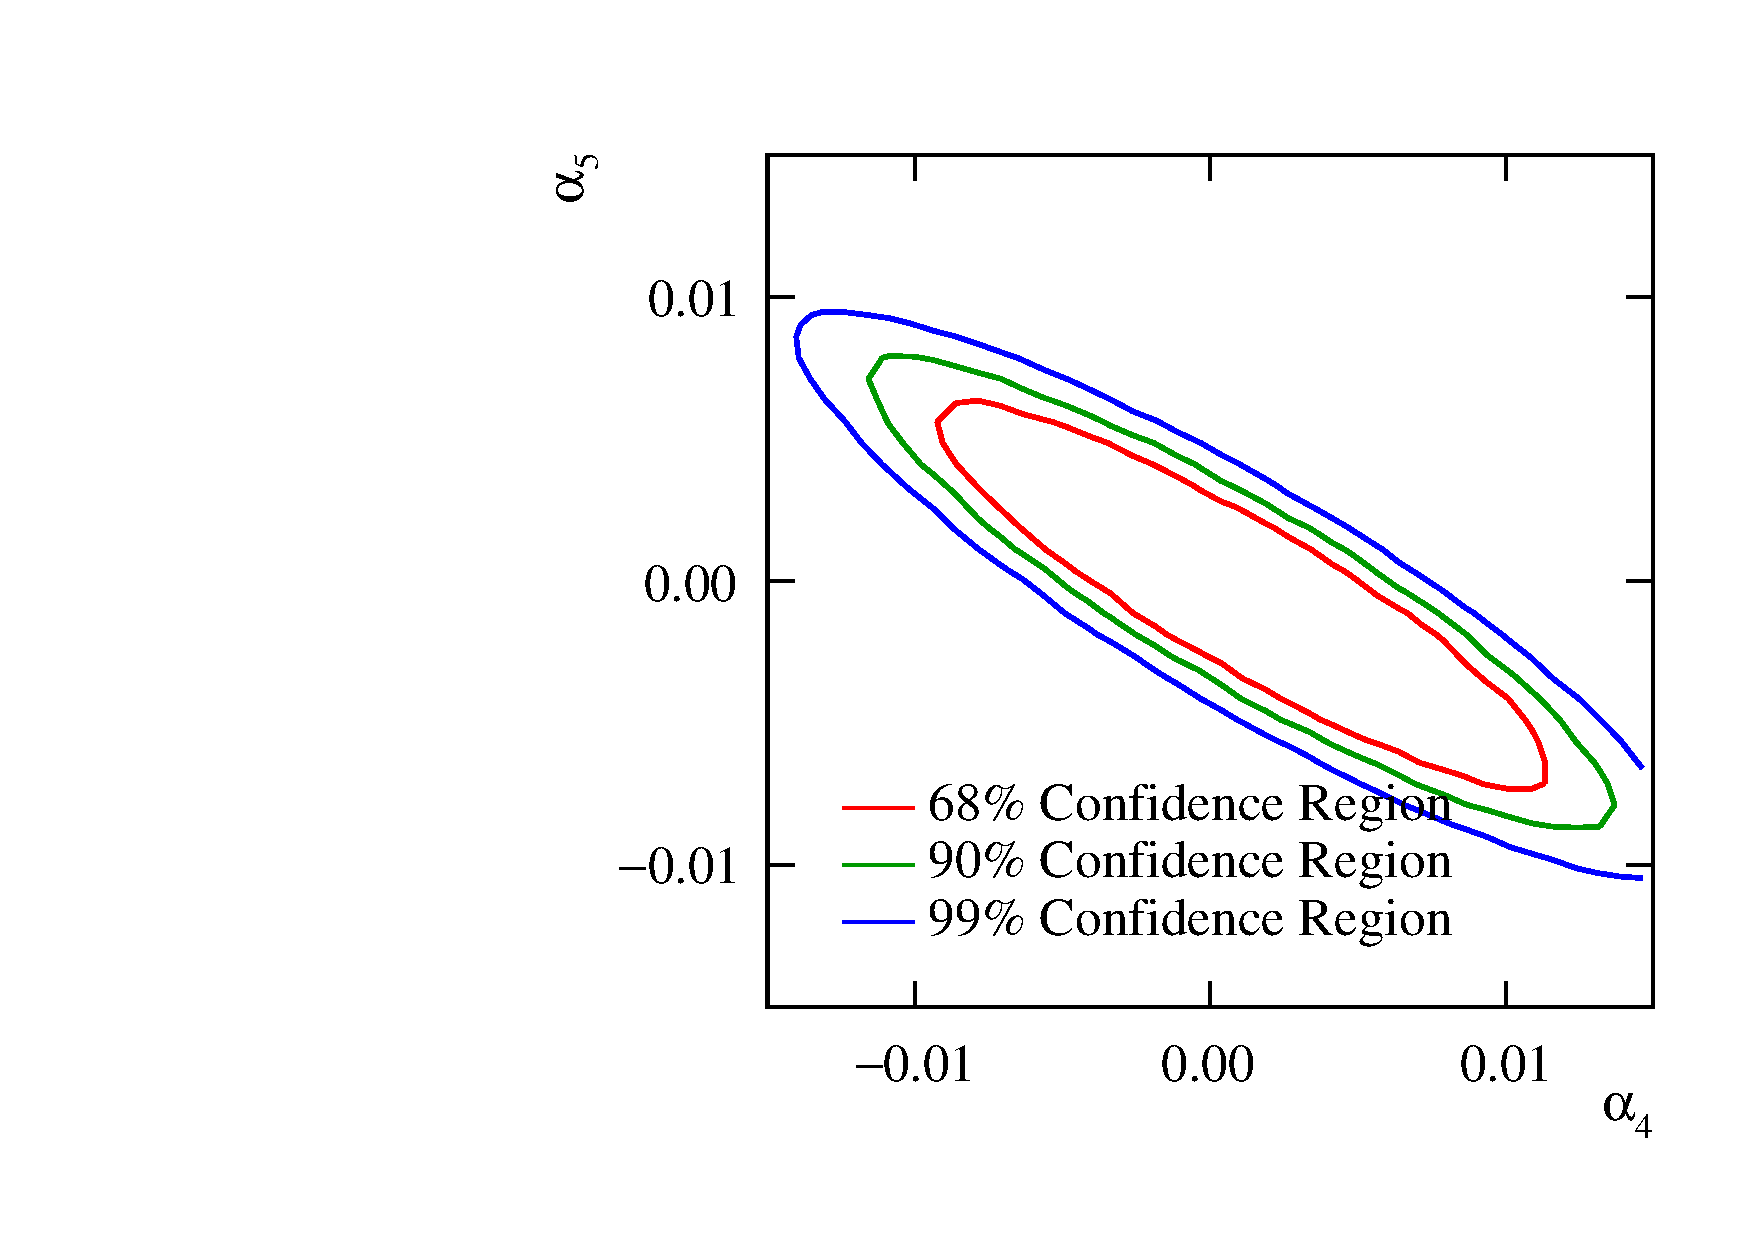
\includegraphics[width=0.5\textwidth]{PhysicsAnalysis/Plots/Chi2ContoursOptimisation/1400GeV/KtSPFOsR0p90_Optimal.pdf}}\hfill
\subfloat[]{\label{fig:a4chi2jetalgoideal1400GeV}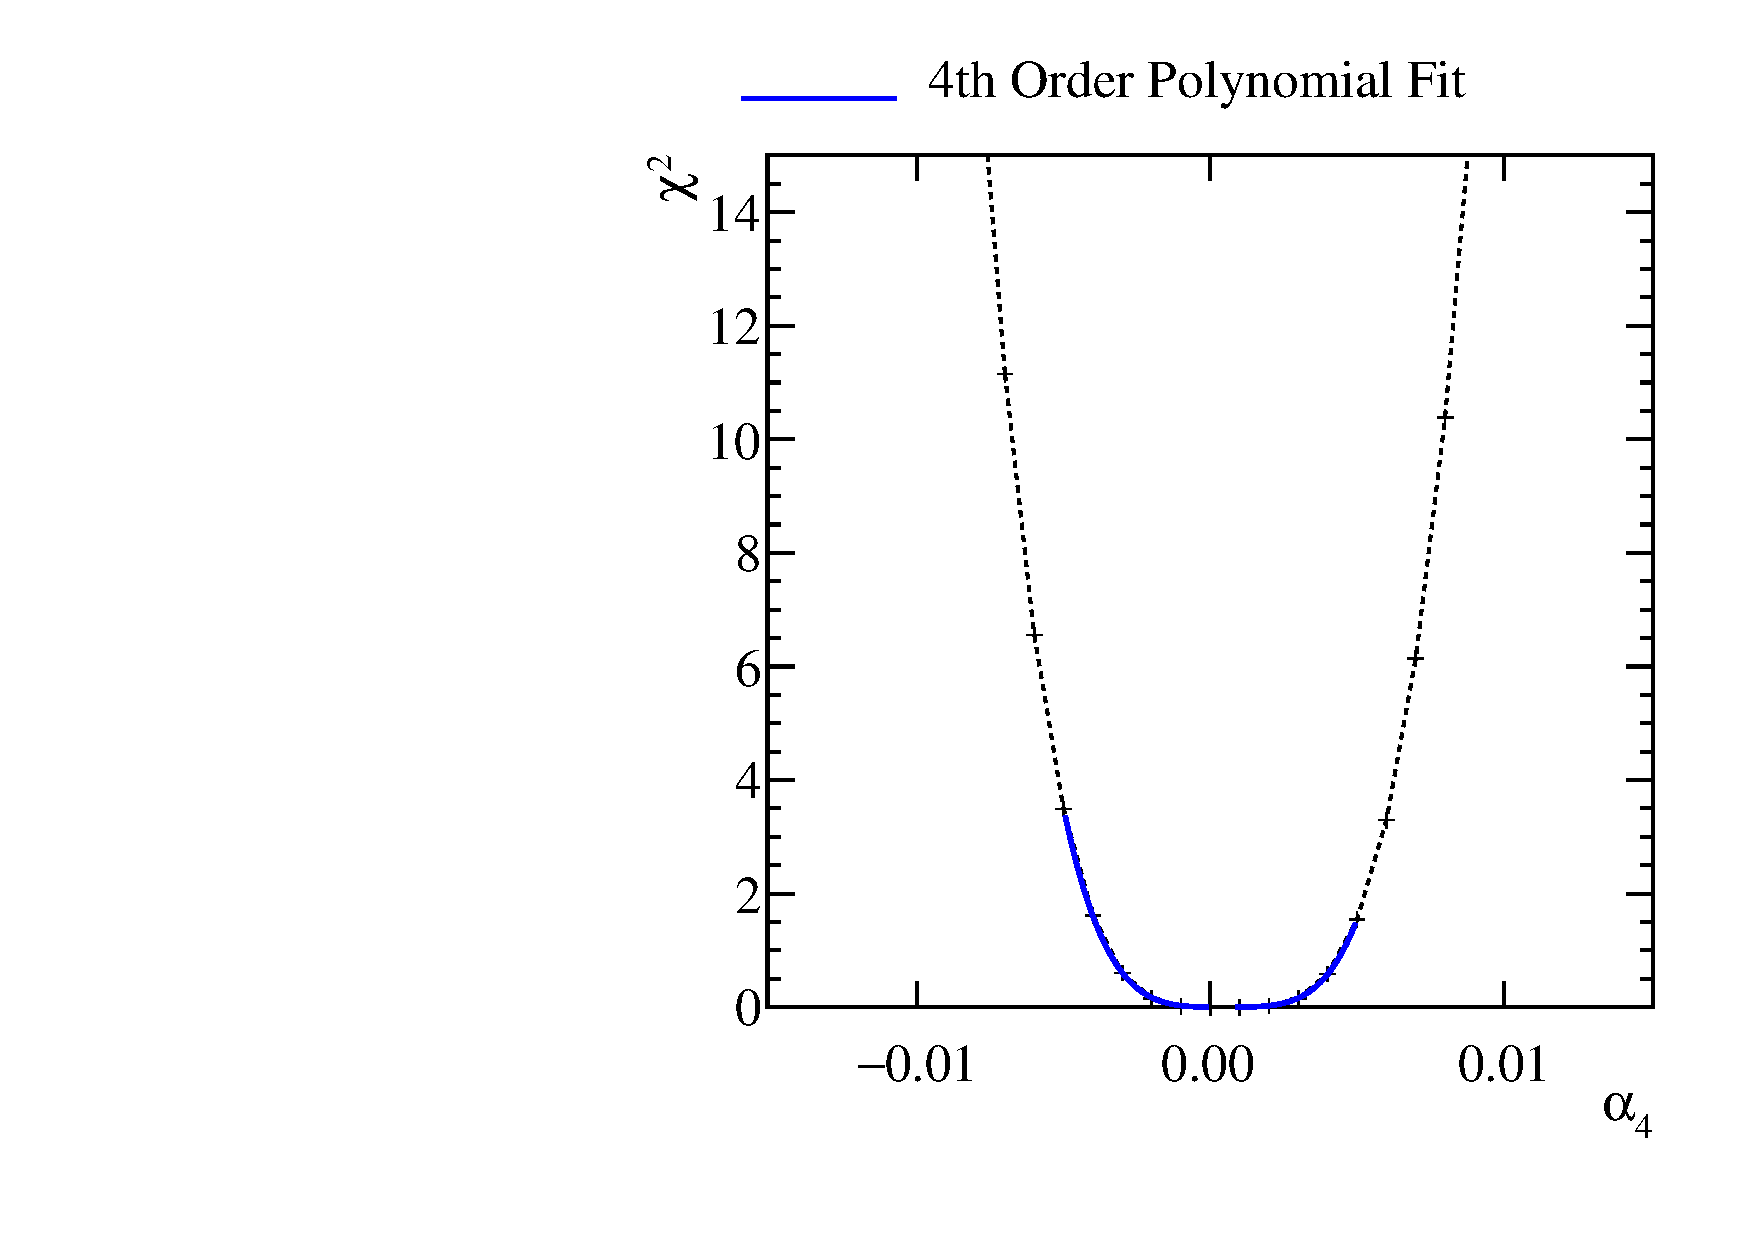
\includegraphics[width=0.5\textwidth]{PhysicsAnalysis/Plots/Chi2ContoursOptimisation/1400GeV/KtSPFOsR0p90_alpha4_Optimal.pdf}}
\subfloat[]{\label{fig:a5chi2jetalgoideal1400GeV}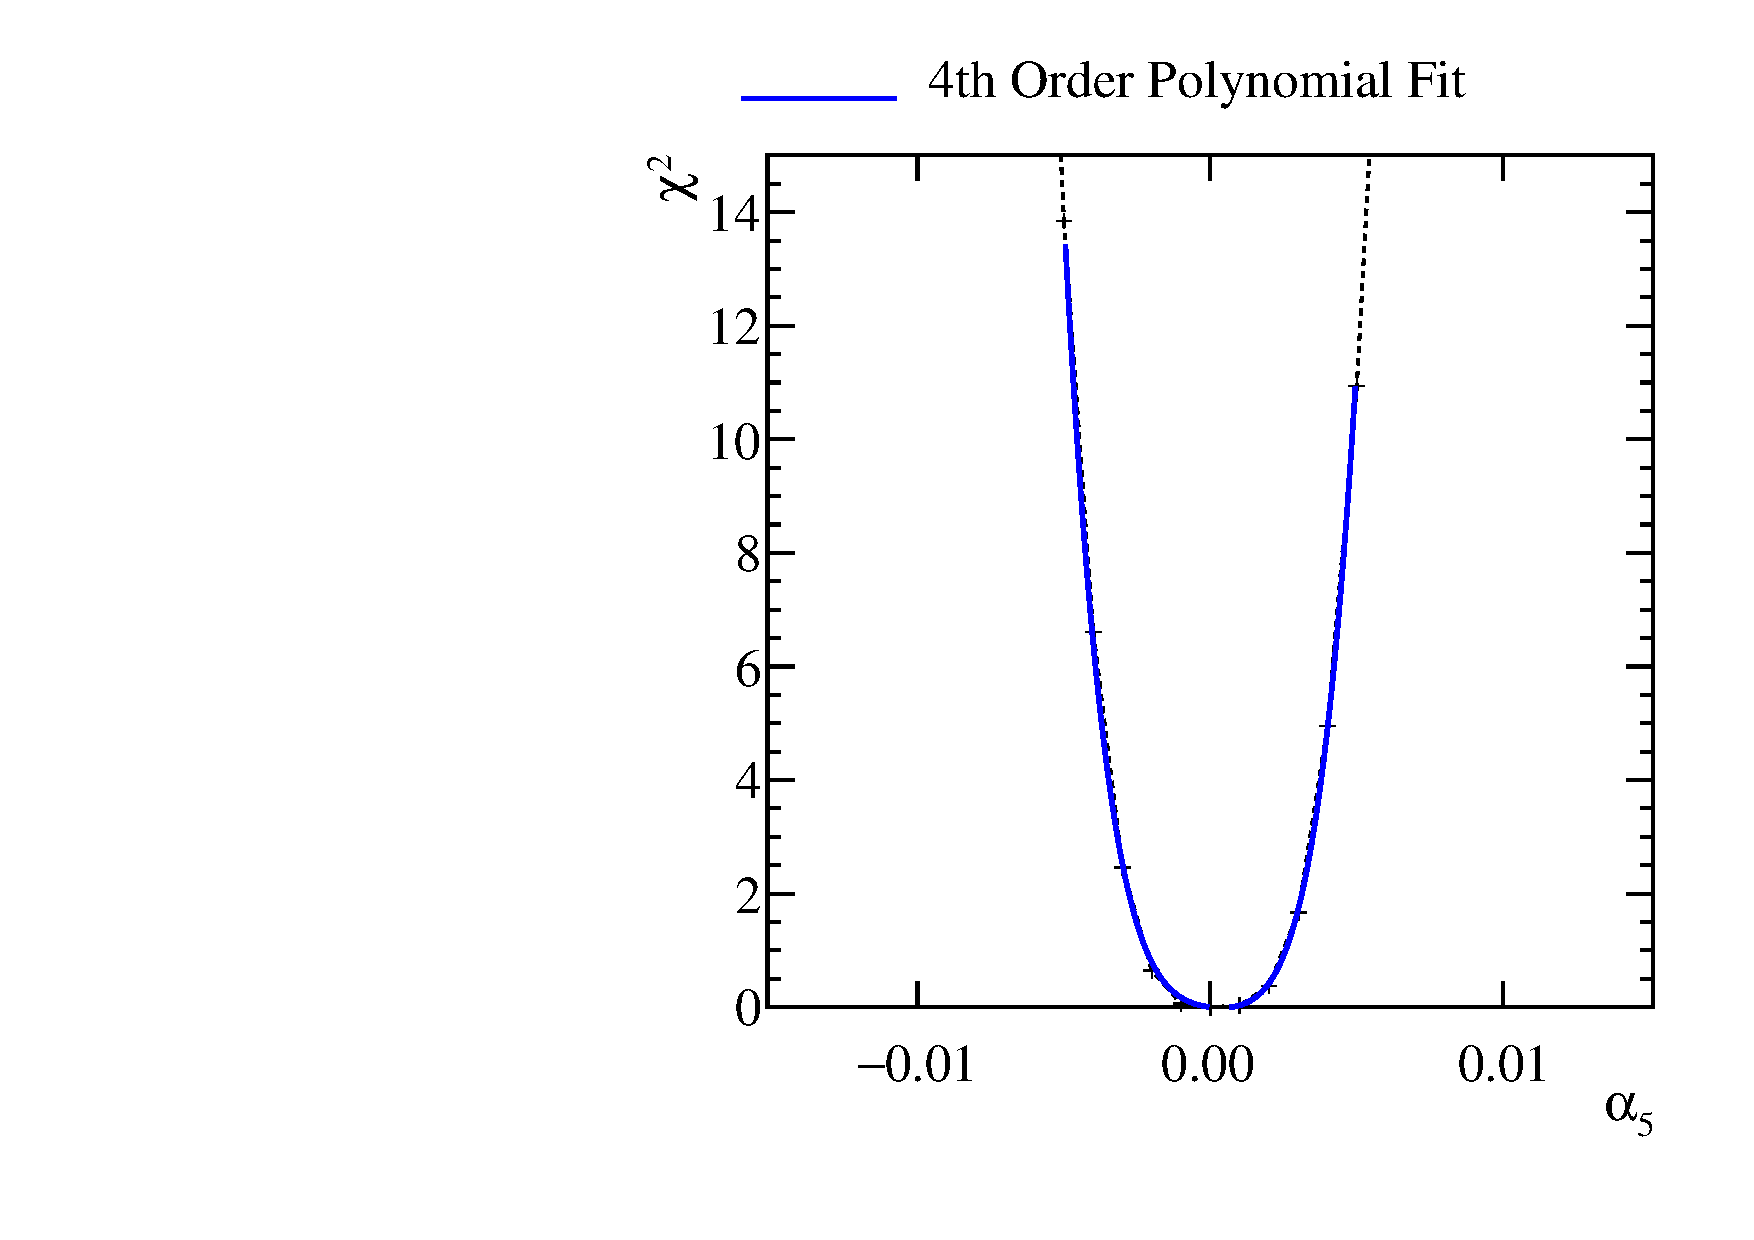
\includegraphics[width=0.5\textwidth]{PhysicsAnalysis/Plots/Chi2ContoursOptimisation/1400GeV/KtSPFOsR0p90_alpha5_Optimal.pdf}}
\caption[$\chi^{2}$ sensitivity distributions from a fit to the invariant mass of the visible system, $M_{VV}$, for the signal {\nu}{\nu}qqqq final state only at $\sqrt{s}=1.4$~TeV.  These results use the optimal jet algorithm configuration of selected PFOs and an R parameter of 0.9 in the $k_{t}$ algorithm.  \protect\subref{fig:chi2jetalgoideal1400GeV} $\chi^{2}$ sensitivity contours in $\alpha_{4}$ and $\alpha_{5}$ space.  \protect\subref{fig:a4chi2jetalgoideal1400GeV} $\chi^{2}$ as a function of $\alpha_{4}$ assuming $\alpha_{5} = 0$.  \protect\subref{fig:a5chi2jetalgoideal1400GeV} $\chi^{2}$ as a function of $\alpha_{5}$ assuming $\alpha_{4} = 0$.  All distributions are normalised to an integrated luminosity of $\mathcal{L}_{int} = 1.5\text{ ab}^{-1}$.]{$\chi^{2}$ sensitivity distributions from a fit to $M_{VV}$ for the signal {\nu}{\nu}qqqq final state only at $\sqrt{s}=1.4$~TeV.  These results use the optimal jet algorithm configuration of selected PFOs and an R parameter of 0.9 in the $k_{t}$ algorithm.  \protect\subref{fig:chi2jetalgoideal1400GeV} $\chi^{2}$ sensitivity contours in $\alpha_{4}$ and $\alpha_{5}$ space.  \protect\subref{fig:a4chi2jetalgoideal1400GeV} $\chi^{2}$ as a function of $\alpha_{4}$ assuming $\alpha_{5} = 0$.  \protect\subref{fig:a5chi2jetalgoideal1400GeV} $\chi^{2}$ as a function of $\alpha_{5}$ assuming $\alpha_{4} = 0$.  All distributions are normalised to an integrated luminosity of $\mathcal{L}_{int} = 1.5\text{ ab}^{-1}$.}
\label{fig:allchi2jetalgoideal1400GeV}
\end{figure}

%========================================================================================

\subsection{Lepton Finding} 
\label{sec:isolatedleptonfinding}
An isolated lepton finder \cite{Wendt:2007iw} was included in the analysis chain to reject background final states containing primary leptons.  Leptons produced via hadronisation are unlikely to be flagged as isolated because all hadronisation products are boosted along the direction of the parent quark.  This means isolated leptons are likely to correspond to primary leptons, which makes the number of isolated leptons a powerful discriminating variable to use in event selection.  

The isolated lepton finder determines whether a PFO is an electron or muon by first checking that the PFO has a single charged particle track associated to it.  If that is the case, the calorimetric energy deposits of the PFO are examined to see if they are consistent with what is expected for an electron or muon.  If they are consistent with expectations, the properties of the charged particle track are examined to determine whether the track originates from the IP.  If the PFO is deemed to have originated from the IP, isolation checks, which examine the energy deposited in the calorimeters within a cone surrounding the PFO, are applied to determine whether the particles belongs to a jet.  If the PFO does not appear to belong to a jet then it is counted as an isolated lepton.  The fraction of events rejected by the lepton finder is summarised in table \ref{table:efficiencyleptonfinding}.   

\begin{table}[h!]
\centering
\begin{tabular}{ l r }
\hline
Final State & $\epsilon_{\text{Lepton Finding}}$ \\ 
\hline
$\text{e}^{+}\text{e}^{-} \rightarrow \nu{\nu}\text{qqqq}$ & 99.7 \\
$\text{e}^{+}\text{e}^{-} \rightarrow \nu\text{lqqqq}$ & 48.9 \\
\hline
\end{tabular}
\caption[The fraction of events rejected by of isolated lepton finding at $\sqrt{s}=1.4$~TeV for the {\nu}{\nu}qqqq and {\nu}lqqqq final states.]{The fraction of events rejected by of isolated lepton finding at $\sqrt{s}=1.4$~TeV for the {\nu}{\nu}qqqq and {\nu}lqqqq final states.}
\label{table:efficiencyleptonfinding}
\end{table}

%========================================================================================

\subsection{Discriminant Variables} 
\label{sec:analysisprocessor}
The next stage of the analysis involved the calculation of a number of event-based variables that were found to be useful for this analysis.  The variables that were calculated are as follows
%
\begin{itemize}
\item \textbf{Particle level} variables:

\begin{itemize}
\item Number of PFOs in each jet;
\item Energy of the highest energy PFO;
\item Energy of the highest energy electron that was identified by PandoraPFA;
\item Cosine of the polar angle of the highest energy track;
\item The number of isolated leptons found using the isolated lepton finder.
\end{itemize}

\item \textbf{Candidate boson} variables:
\begin{itemize}
\item Energy of the candidate bosons;
\item Invariant mass of the candidate bosons;
\item Acolinearity of the candidate boson pair, which is defined as 180 degrees minus the opening angle of the pair of bosons in the rest frame of the detector.
\end{itemize}

\item \textbf{Event based} variables:  
\begin{itemize}
\item The invariant mass of the visible system, $M_{VV}$;
\item The vector sum of the transverse momentum of all PFOs in the event;
\item Sphericity, defined through the sphericity tensor $S^{ab}$;
\begin{equation}
S^{ab} = \frac{\Sigma_{i}p^{\alpha}_{i}p^{\alpha}_{j}}{\Sigma_{i,\alpha=1,2,3}|p^{\alpha}_{i|^{2}}}
\end{equation}
where $p_{i}$ are the components of the momenta of the $i^{th}$ PFO in the rest frame of the detector and the sum $\Sigma_{i}$ runs over all particles in the event.  Sphericity is defined as $S = (3/2)(\lambda_{2} + \lambda_{3})$, where $\lambda_{i}$ are the eigenvalues of the sphericity tensor defined such $\lambda_{1} \geq \lambda_{2} \geq \lambda_{3}$.  This provides a measure of how spherical the reconstructed event topology is with isotropic events having $S \approx 1$, while two jet events have $S \approx 0$.
\end{itemize}

\item \textbf{Jet clustering parameters} variables:
\begin{itemize}
\item The $y_{ij}$ variables where $i = 3,4$ and $j=i+1$.  These are the smallest $k_{t}$ distance found when combining $j$ jets into $i$ jets.  
\end{itemize}
\end{itemize}

%========================================================================================

\subsection{Jet Energy Resolution at CLIC} 
\label{sec:jetenergyresolution}
The importance of the jet energy resolution, which is extensively discussed in chapters \ref{chapt:energyestimators} and \ref{chap:detopt}, should be emphasised at this point.  Many of the discriminant variables that are calculated for this analysis are dependant upon the jet energy resolution.  In particular, all variables related to the candidate bosons, which are formed from pairing up jets, are dependent upon the measurement of jet energies.  

Figure \ref{fig:jeteenrgyresolutionphysicsanalysis} shows the jet energy resolution as a function of the MC jet energy for the {\nu}{\nu}qqqq event sample used in the $\sqrt{s}=1.4$~TeV analysis.  The MC jet energy was obtained by pairing up quarks appearing in the final state to the reconstructed jets.  The events were then binned in terms of their MC jet energy and the jet energy resolution calculated for each bin.  When calculating the jet energy resolution, a narrower range of jet energies was used in compared to previous studies, 60\% of the data with narrowest RMS as opposed to 90\%, to minimise the effects of jet finding and beam-induced backgrounds.  The jet energy resolutions reported here are worse than those quoted in earlier chapters.  This is to be expected given the effects of jet finding and beam-induced backgrounds.

\begin{figure}
\centering
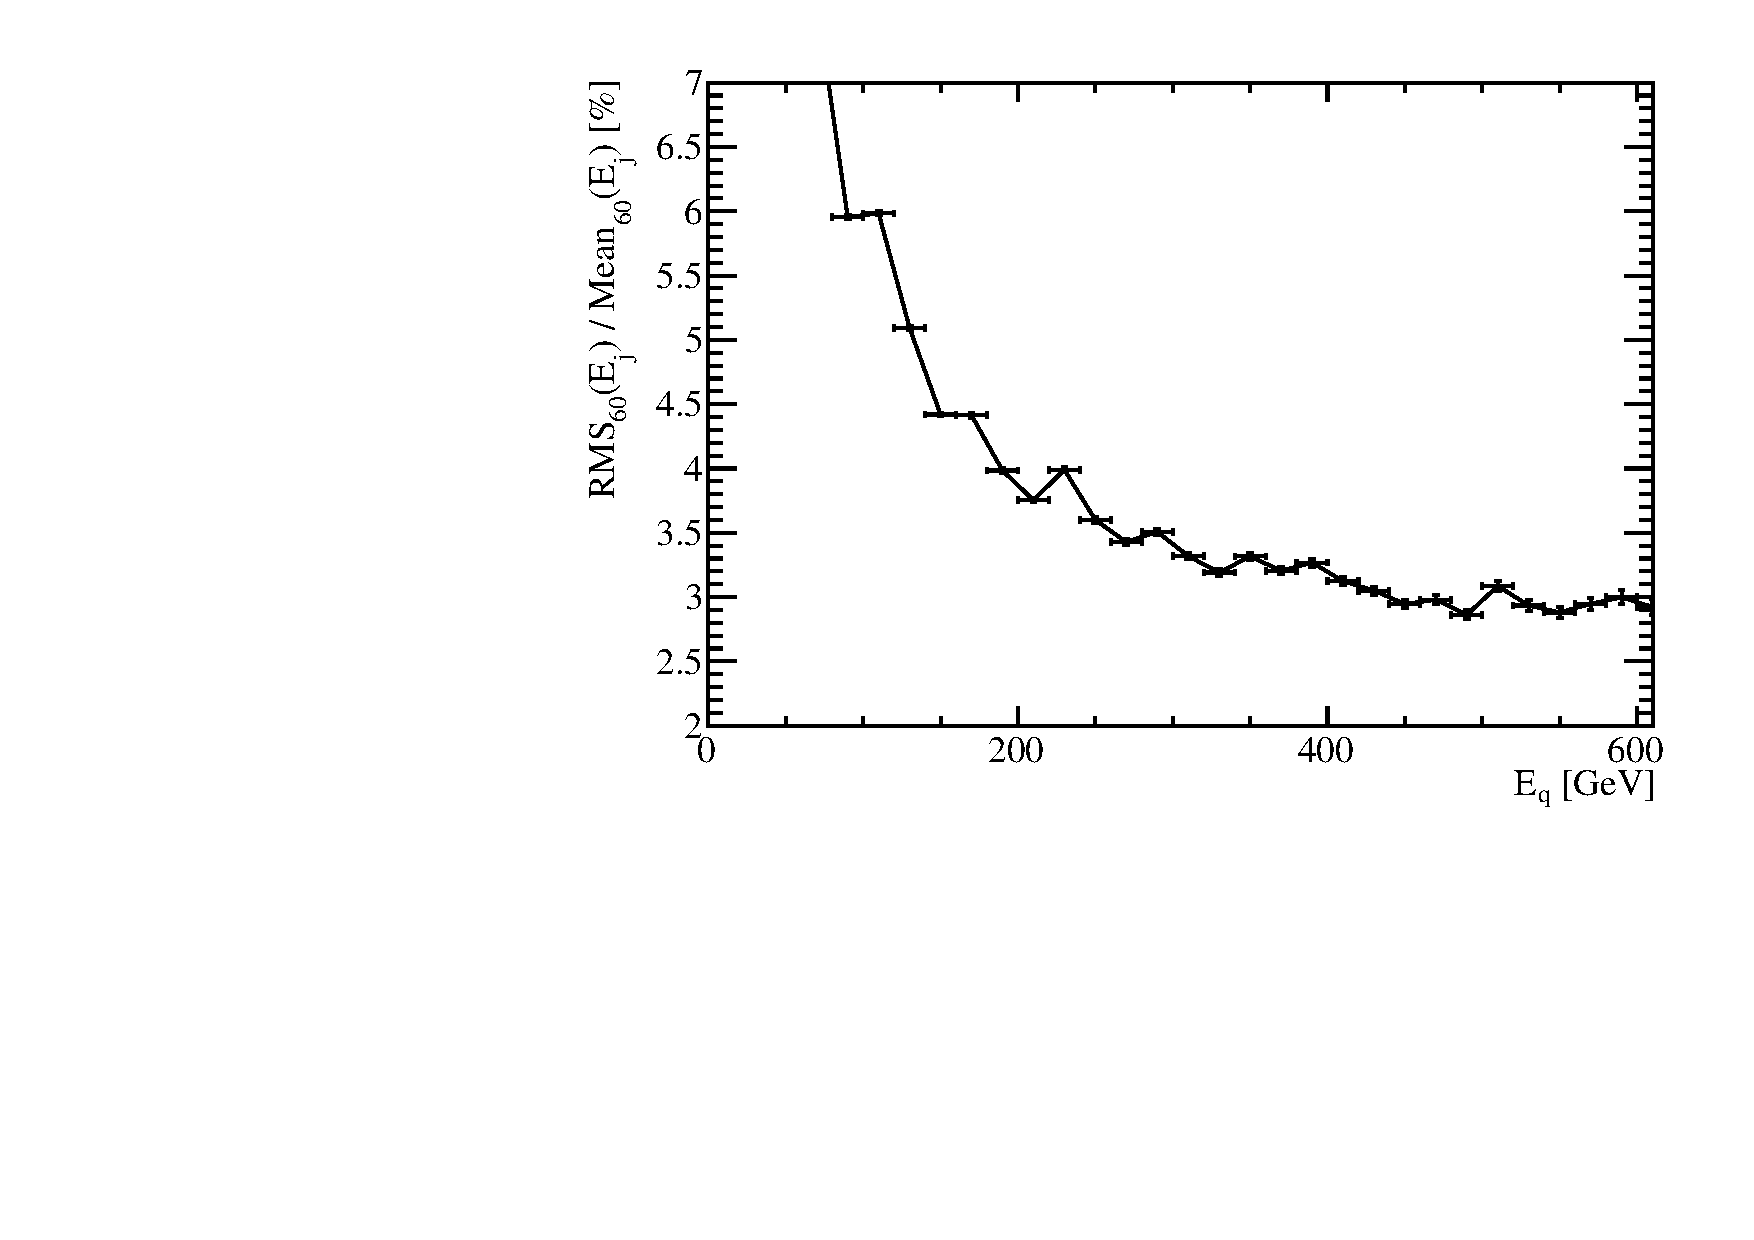
\includegraphics[width=0.75\textwidth]{PhysicsAnalysis/Plots/JetEnergyResolution/JetEnergyResolutionScan_1400GeV.pdf}
\caption[The jet energy resolution as a function of the jet energy for the {\nu}{\nu}qqqq final state at $\sqrt{s}=1.4$~TeV.]{The jet energy resolution as a function of the jet energy for the {\nu}{\nu}qqqq final state at $\sqrt{s}=1.4$~TeV.}
\label{fig:jeteenrgyresolutionphysicsanalysis}
\end{figure}

%========================================================================================
%========================================================================================

\section{Event Selection}
\label{sec:eventselection}
This section discusses the event selection procedure.  The goal of this procedure is to isolate the \nu{\nu}qqqq final state from the background final states, i.e. those containing two and four primary quarks.  The procedure consists of a set of preselection cuts followed by the application of a multivariate analysis (MVA).  All event numbers  have been normalised, prior to event selection, to an integrated luminosity of $\mathcal{L}_{int} = 1.5\text{ ab}^{-1}$ for the $\sqrt{s} = 1.4$~TeV analysis and $\mathcal{L}_{int} = 2\text{ ab}^{-1}$  for the $\sqrt{s} = 3$~TeV analysis.  

%========================================================================================

\subsection{Preselection}
\label{sec:preselection1400GeV}
A refined selection of the \nu{\nu}qqqq signal final state is achieved using a MVA, however, to ensure efficiency in the training and application of that MVA a number of simple preselection cuts were developed to veto obvious background final states prior to the application of the MVA.  Preselection cuts were applied to the transverse momentum of the system and the number of isolated leptons found in the event.  The raw distributions of these variables is shown in figure \ref{fig:preselection1400} and based on these distributions the following cuts were applied
%
\begin{itemize}
\item Transverse momentum of system > 100~GeV.  This cut is effective due to the presence of missing energy in the form of neutrinos in the signal final state.
\item Number of isolated leptons in system = 0.  This cut is effective as the signal final state does not contain leptons, while numerous background final states do.  
\end{itemize}
%
\noindent The impact of these preselection cuts can be found in table \ref{table:selectionsummary1400GeV}, which can be found on page \pageref{table:selectionsummary1400GeV}.

\begin{figure}[h!]
\centering
\subfloat[]{\label{fig:preselection1400_1}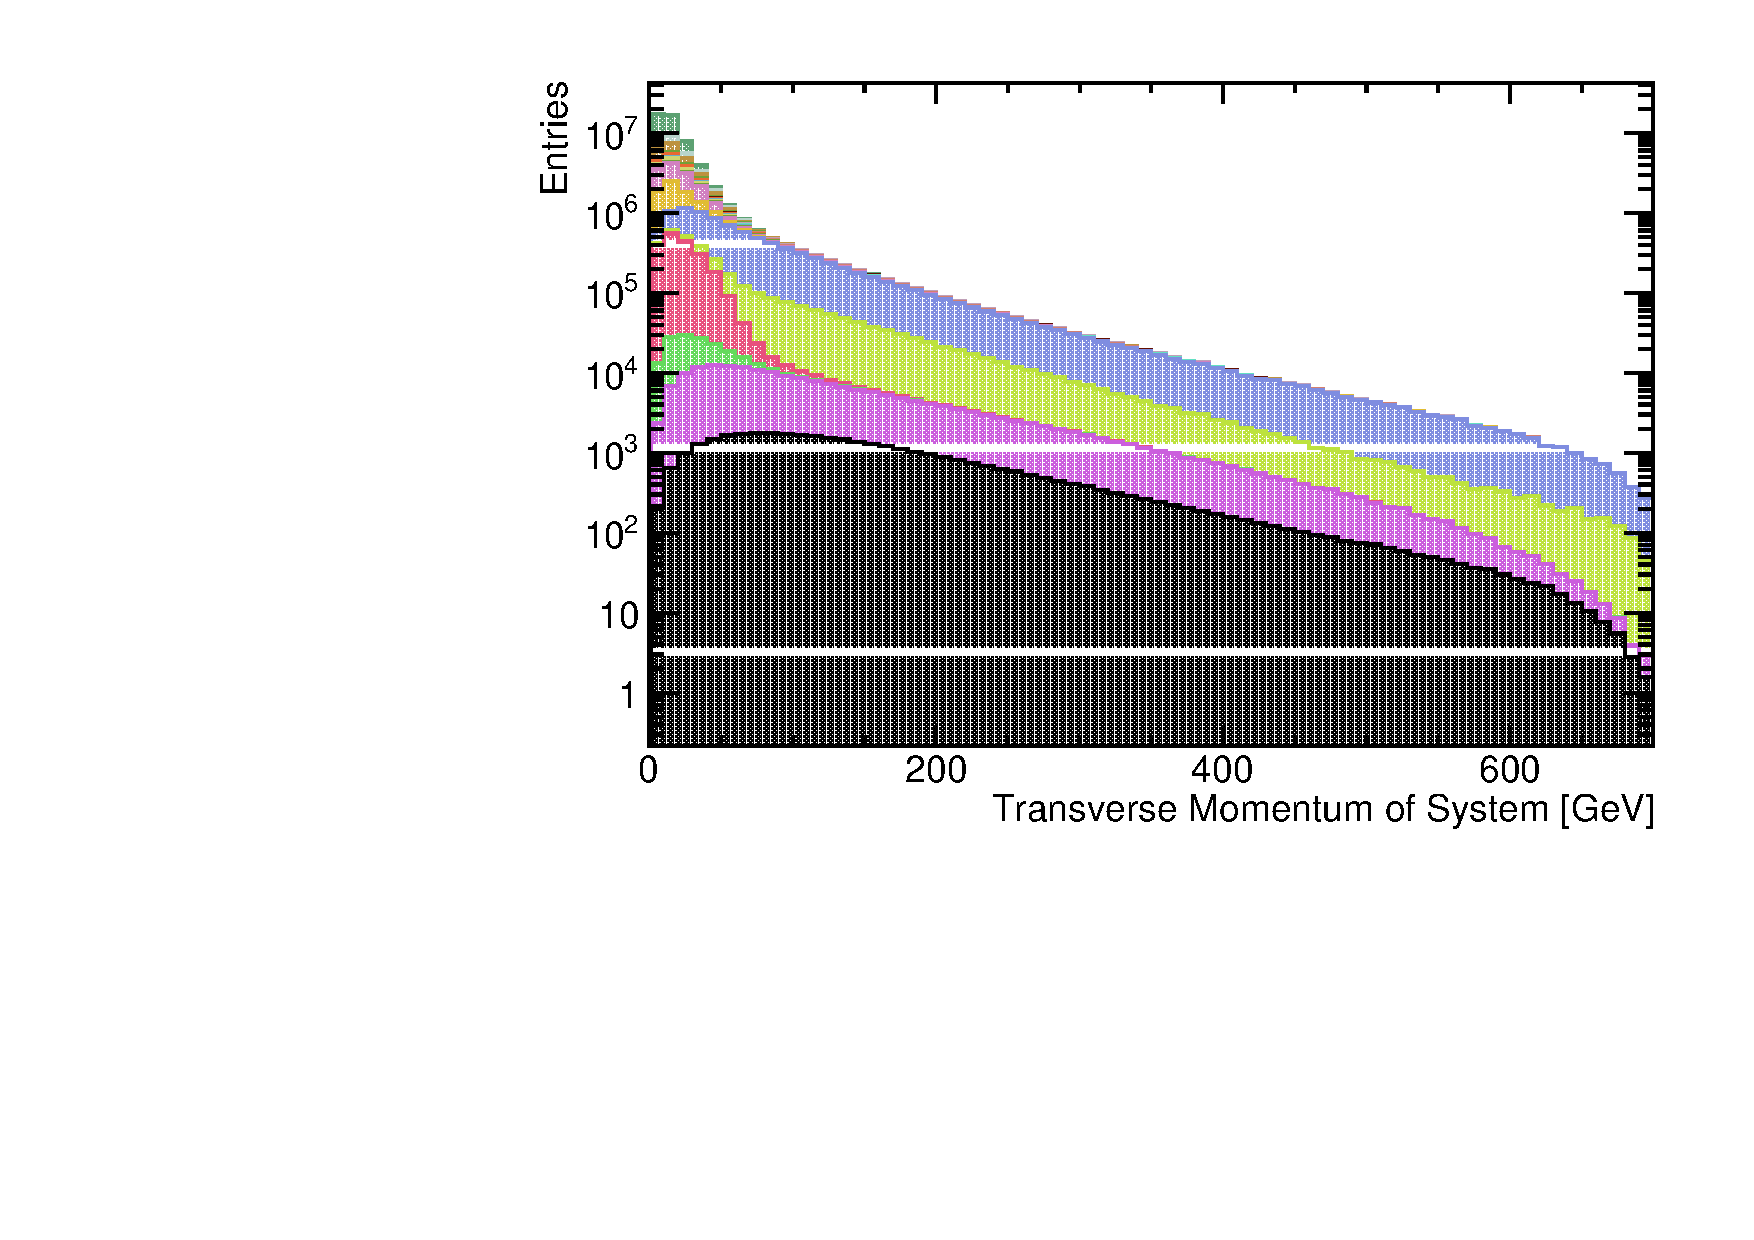
\includegraphics[width=0.5\textwidth]{PhysicsAnalysis/Plots/PreSelection/1400GeV/TransverseMomentum.pdf}}
\subfloat[]{\label{fig:preselection1400_2}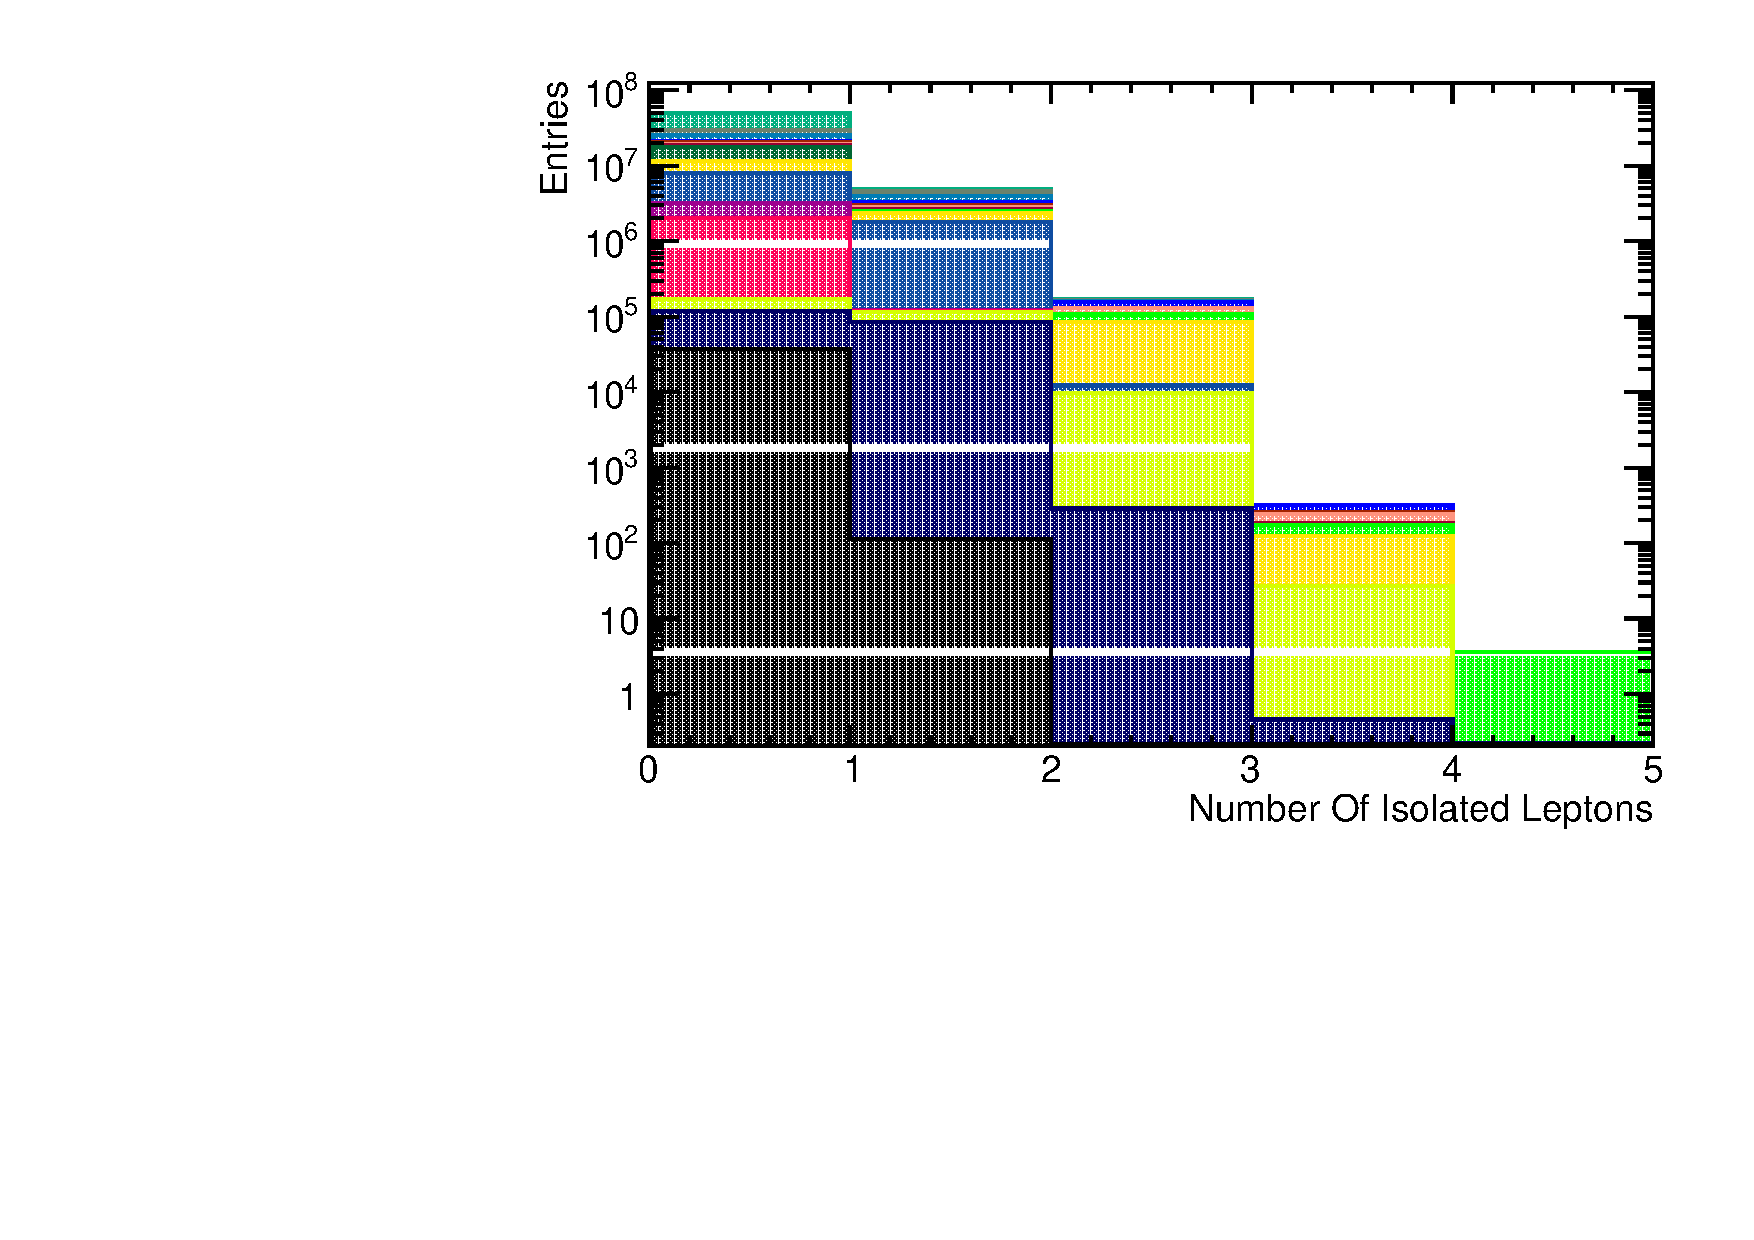
\includegraphics[width=0.5\textwidth]{PhysicsAnalysis/Plots/PreSelection/1400GeV/NumberOfIsolatedLeptons.pdf}} \hfill
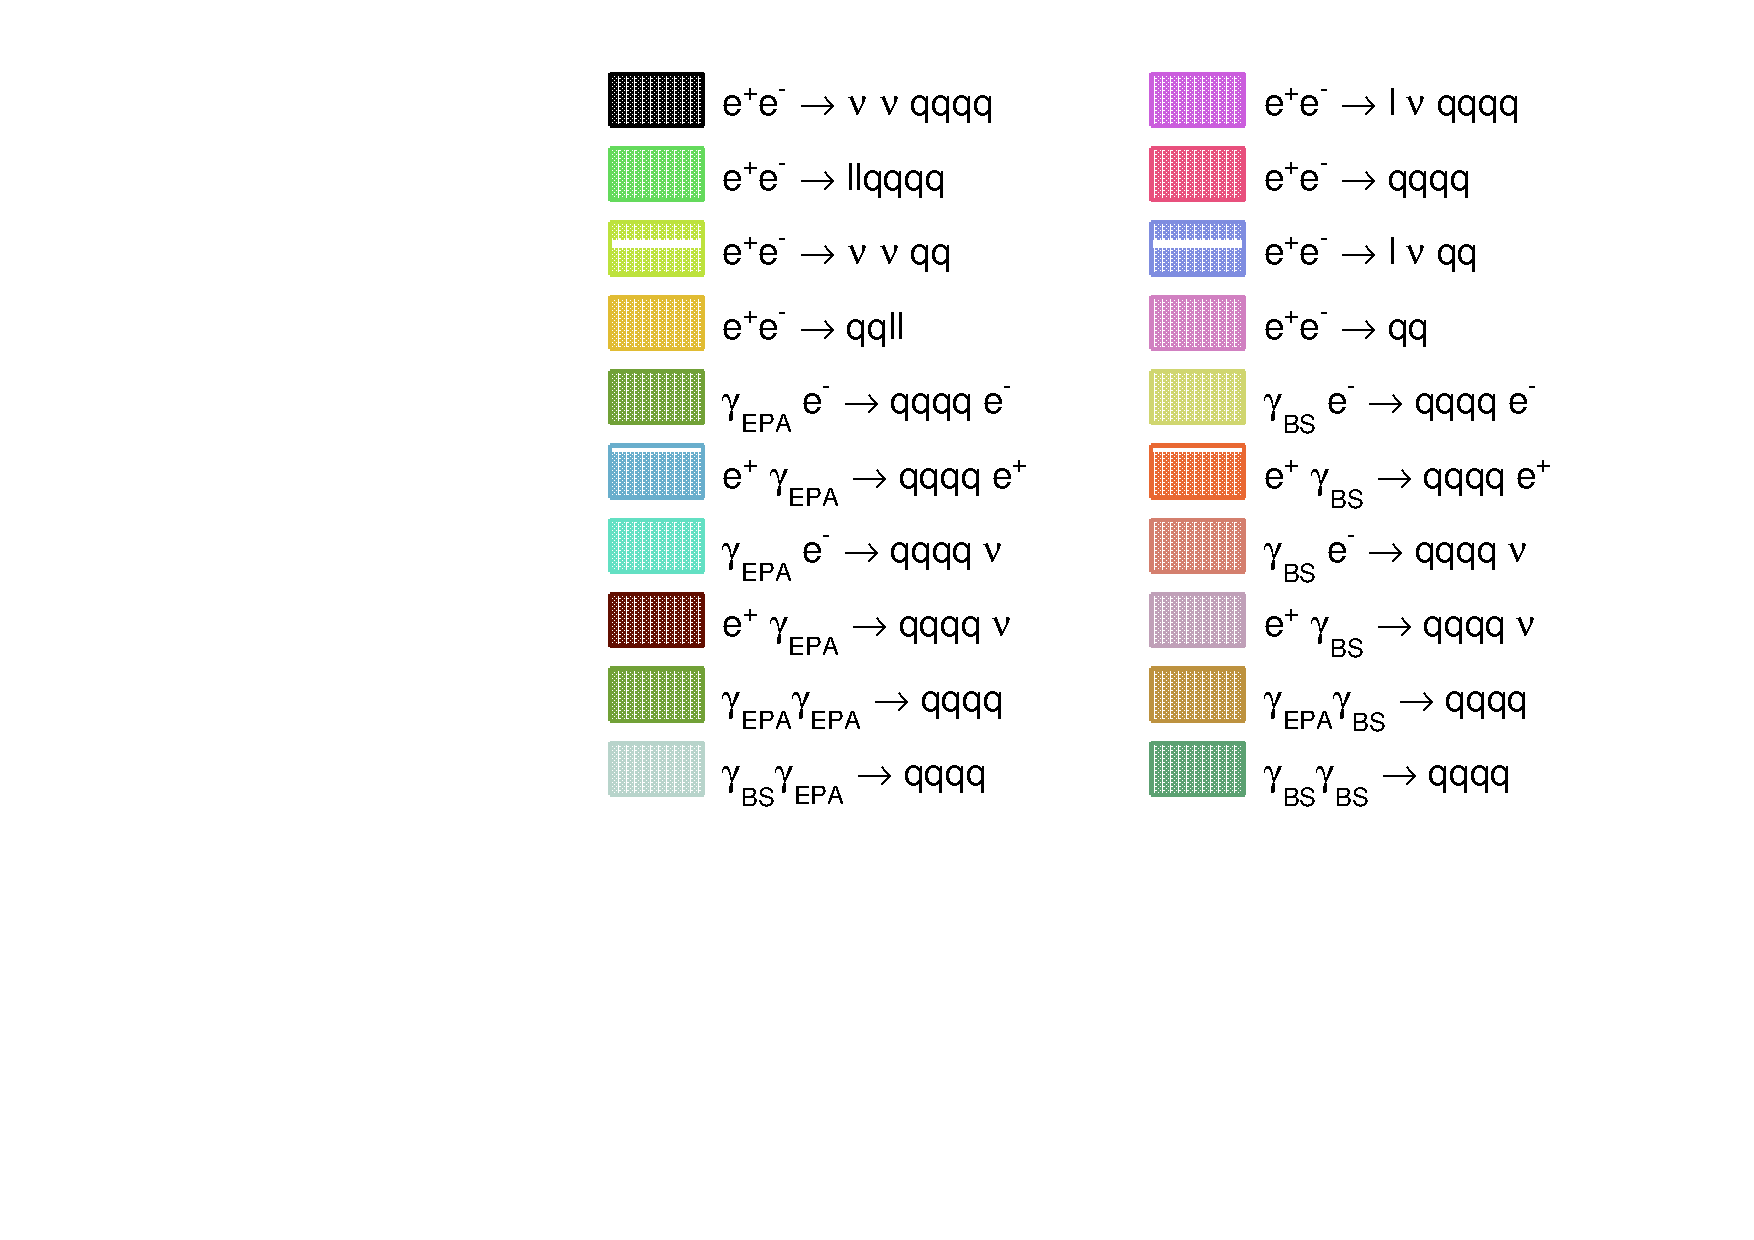
\includegraphics[width=0.5\textwidth]{PhysicsAnalysis/Plots/PreSelection/1400GeV/Legend.pdf}
\caption[Distribution of the preselection cut variables at $\sqrt{s}=1.4$~TeV: \protect\subref{fig:preselection1400_1} the transverse momentum of the visible system; and \protect\subref{fig:preselection1400_2} the number of isolated leptons in the system.  All distributions are normalised to an integrated luminosity of $\mathcal{L}_{int} = 1.5\text{ ab}^{-1}$.]{Distribution of the preselection cut variables at $\sqrt{s}=1.4$~TeV: \protect\subref{fig:preselection1400_1} the transverse momentum of the visible system; and \protect\subref{fig:preselection1400_2} the number of isolated leptons in the system.  All distributions are normalised to an integrated luminosity of $\mathcal{L}_{int} = 1.5\text{ ab}^{-1}$.}
\label{fig:preselection1400}
\end{figure}

%========================================================================================

\subsection{Multivariate analysis}
\label{sec:mva1400GeV}
Having established the preselection cuts, a MVA was applied using the TMVA toolkit \cite{Hocker:2007ht}, to refine the event selection.  The signal and background final state samples were separated into two equally sized samples; one sample was used to independently train the MVA and the other sample was used in the subsequent analysis.  

The performance of several MVA classifiers was examined to determine the optimal classifier for this analysis.  The MVA classifiers considered were \cite{Hocker:2007ht}:
\begin{itemize}
\item \textbf{Boosted Decision Tree (BDT)}.  Decision trees are formed by the sequential application of cuts that split the data into multiple classes.  After the application of the final cut, the remaining classes are used to classify whether the input event corresponds to signal or background.  Boosting a decision tree involves the use of several decision trees.  A single classifier output is obtained from a weighted average of the individual decision trees.  The cuts applied in the decision tree are determined using the training sample.  
\item \textbf{$k$-Nearest Neighbour (KNN)}.  For a given input event, the $k$ closest neighbours from the training sample are found.  The classifier for that input event is determined as the fraction of those $k$ events that belong to the signal sample.  Distances in this classifier are defined as the Euclidean distance between events in the $n$-dimensional space of the variables used for training the classifier.  Weights are applied when calculating the distances to account for the differing widths of the input variable distributions.  The value of $k$ used in this analysis was 20.
\item \textbf{Multilayer Perceptron (MLP)}.  This is an example of a neutral network.  Neutral networks consist of an interconnected series of neurons each with a different response to a set of input signals.  The signal for the first layer of neurons are the event variables used to train the MVA.  The input signal proceeds to travel through several layers of neurons.  The number of neurons in a given layer is reduced as the number of layers passed through increases until two neurons are left, one corresponding to signal and the other background.  The neuron giving the larger response in the final layer determines the event classifier.  The training sample is used to determine the response of each neurons in the network.
\item \textbf{Fisher and H-Matrix Discriminants}.  These procedures involve the calculation of a hyperplane in $n$-dimensional space that maximally separates signal and background events in the training sample.  The location of an input event in that $n$-dimensional space with respect to that hyperplane determines the classifier for the event.  The hyperplane is determined by maximising the differences between the means of the input event variables normalised by a measure of their spread.  Both the Fisher and H-Matrix discriminants search for the hyperplane in $n$-dimensional space, however, the Fisher discriminant begins this procedure by transforming the input variables into a variable space with no linear correlations.  
\item \textbf{Likelihood}.  The likelihood is determined using the probability density function (PDF) for each of the input variables.  PDFs are determined using the training sample for both signal and background events.  For a given event, the likelihood is given by the product of the probability of obtaining each of the input variables for that event.  The signal and background likelihoods are calculated using the signal and background PDFs respectively and the ratio of the signal likelihood to the sum of the signal and background likelihoods gives the event classifier.   
\end{itemize}

The input variables used for these MVA classifiers were:
\begin{itemize}
\item Number of PFOs in each jet;
\item Energy of the highest energy PFO;
\item Energy of the highest energy electron;
\item Cosine of the polar angle of the highest energy track;
\item Energy of the candidate bosons;
\item Invariant mass of the candidate bosons;
\item Acolinearity of the candidate boson pair;
\item The vector sum of the transverse momentum of all PFOs in the event;
\item The sphericity of the event;
\item The derived jet clustering parameter variables $-\text{log}_{10}(y_{ij})$ where $y_{ij}$ are jet clustering parameters, $i = 3,4$ and $j=i+1$.  
\end{itemize}

Figure \ref{fig:mvaalternatives1400GeV} shows the background rejection, which is equivalent to one minus the background efficiency, as a function of signal efficiency for various MVA classifiers.  Efficiency is defined as the fraction of events classified as signal by the MVA.  The efficiencies reported by TMVA are calculated after the application of the preselection cuts, which are described in section \ref{sec:preselection1400GeV}.  

The classifier giving the optimal performance in terms of signal efficiency and background rejection was the BDT.  The performance of the BDT was optimised further by varying the number of trees used and the depth of the trees.  An optimal significance, S/$\sqrt(\text{S + B})$, where S and B are the number of signal and background events passing the preselection respectively, of 52.7 was obtained using the BDT.  \textcolor{blue}{Table \ref{table:mvaranking1400GeV} shows the ranking of the variables used by the BDT and figure \ref{fig:rankingvariables} shows the distributions of the three highest ranked variables.}

\begin{figure}
\centering
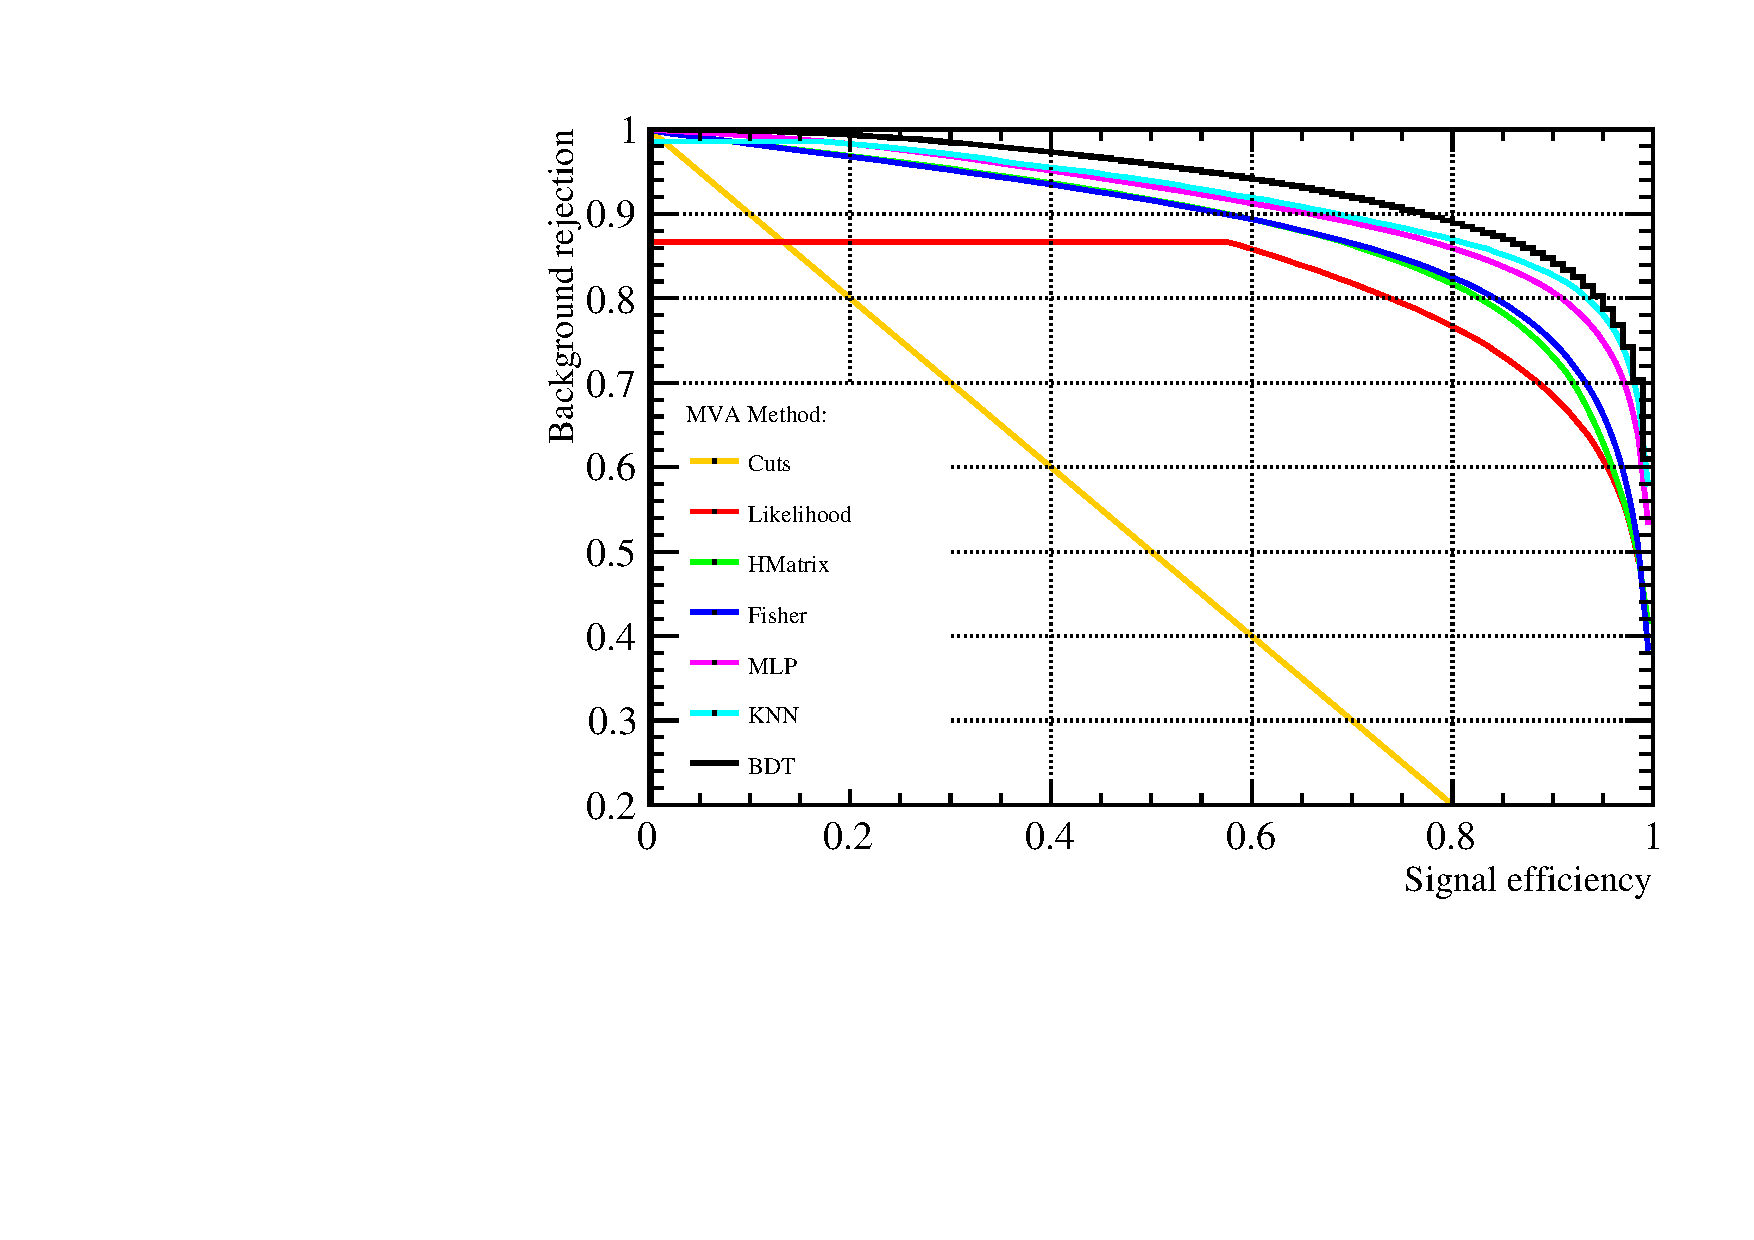
\includegraphics[width=0.75\textwidth]{PhysicsAnalysis/Plots/MVAPlots/1400GeV/ThesisPlotMVAAlternatives1400GeV.pdf}
\caption[Background rejection as a function of signal efficiency for a variety of MVA options at $\sqrt{s}=1.4$~TeV.]{Background rejection as a function of signal efficiency for a variety of MVA options at $\sqrt{s}=1.4$~TeV.} 
\label{fig:mvaalternatives1400GeV}
\end{figure}

\begin{table}[h!]
\centering
\begin{tabular}{ l r }
\hline
MVA Variable & Ranking \\
\hline
Acolinearity of the candidate boson pair & 1 \\
Invariant mass of the highest energy candidate boson & 2 \\
Number of particles in the highest energy jet & 3 \\
Energy of the lowest energy candidate boson & 4 \\
Energy of the highest energy PFO & 5 \\
Invariant mass of the lowest energy candidate boson & 6 \\
Jet clustering parameter $-\text{log}_{10}(y_{34})$ & 7 \\
Energy of the highest energy candidate boson & 8 \\
Number of particles in the second highest energy jet & 9 \\
Sphericity of the event & 10 \\
Number of particles in the third highest energy jet & 11 \\
Energy of the highest energy electron & 12 \\
Cosine of the polar angle of the highest energy track & 13 \\
Number of particles in the fourth highest energy jet & 14 \\
The vector sum of the transverse momentum of all PFOs in the event & 15 \\
Jet clustering parameter $-\text{log}_{10}(y_{45})$ & 16 \\
\hline
\end{tabular}
\caption[Ranking of the MVA variables used by the BDT.]{\textcolor{blue}{Ranking of the MVA variables used by the BDT.}}
\label{table:mvaranking1400GeV}
\end{table}

\begin{figure}[h!]
\centering
\subfloat[]{\label{fig:ranking1}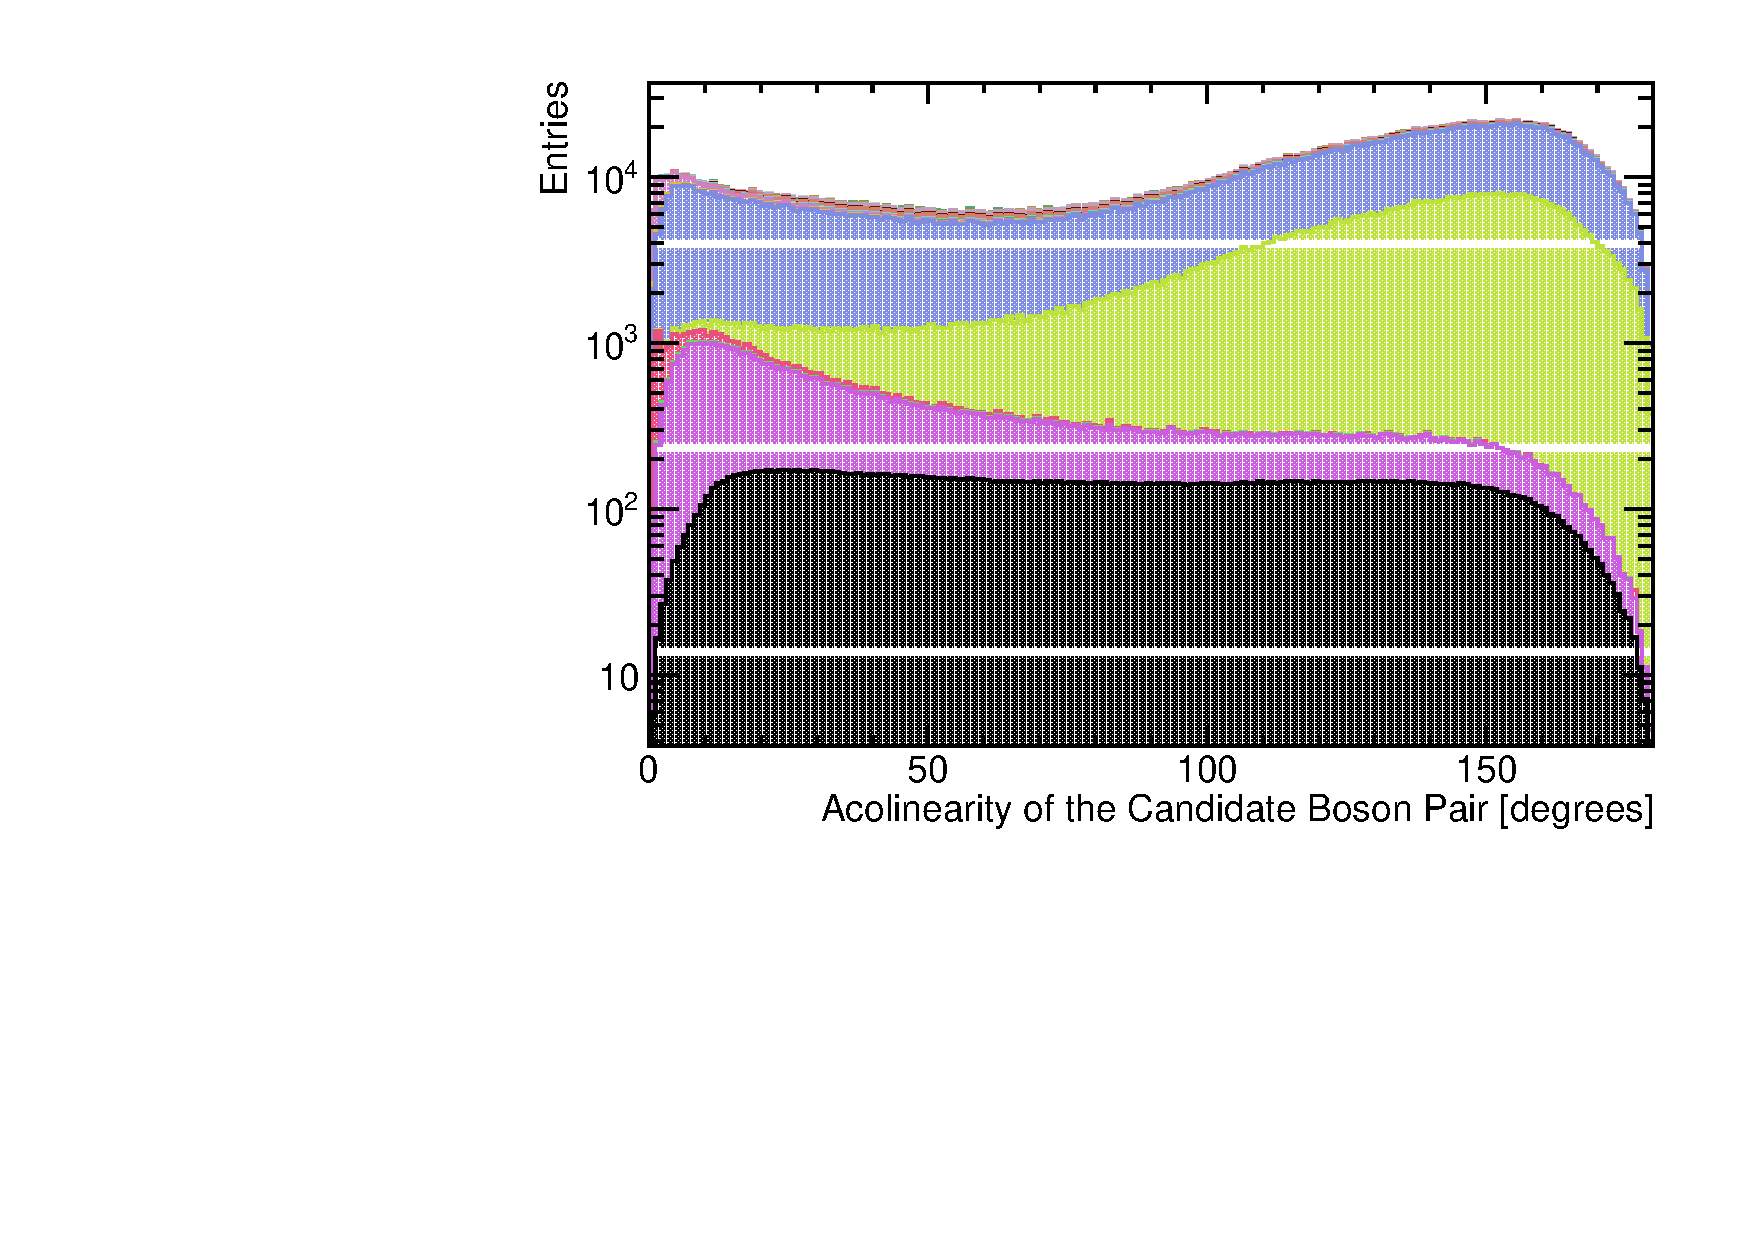
\includegraphics[width=0.5\textwidth]{PhysicsAnalysis/Plots/HighRankingVariables/1400GeV/AcolinearitySynBosons_1400GeV_Pt_gt100GeV_NIsoLep_eq0_Cuts_StackPlot.pdf}}
\subfloat[]{\label{fig:ranking2}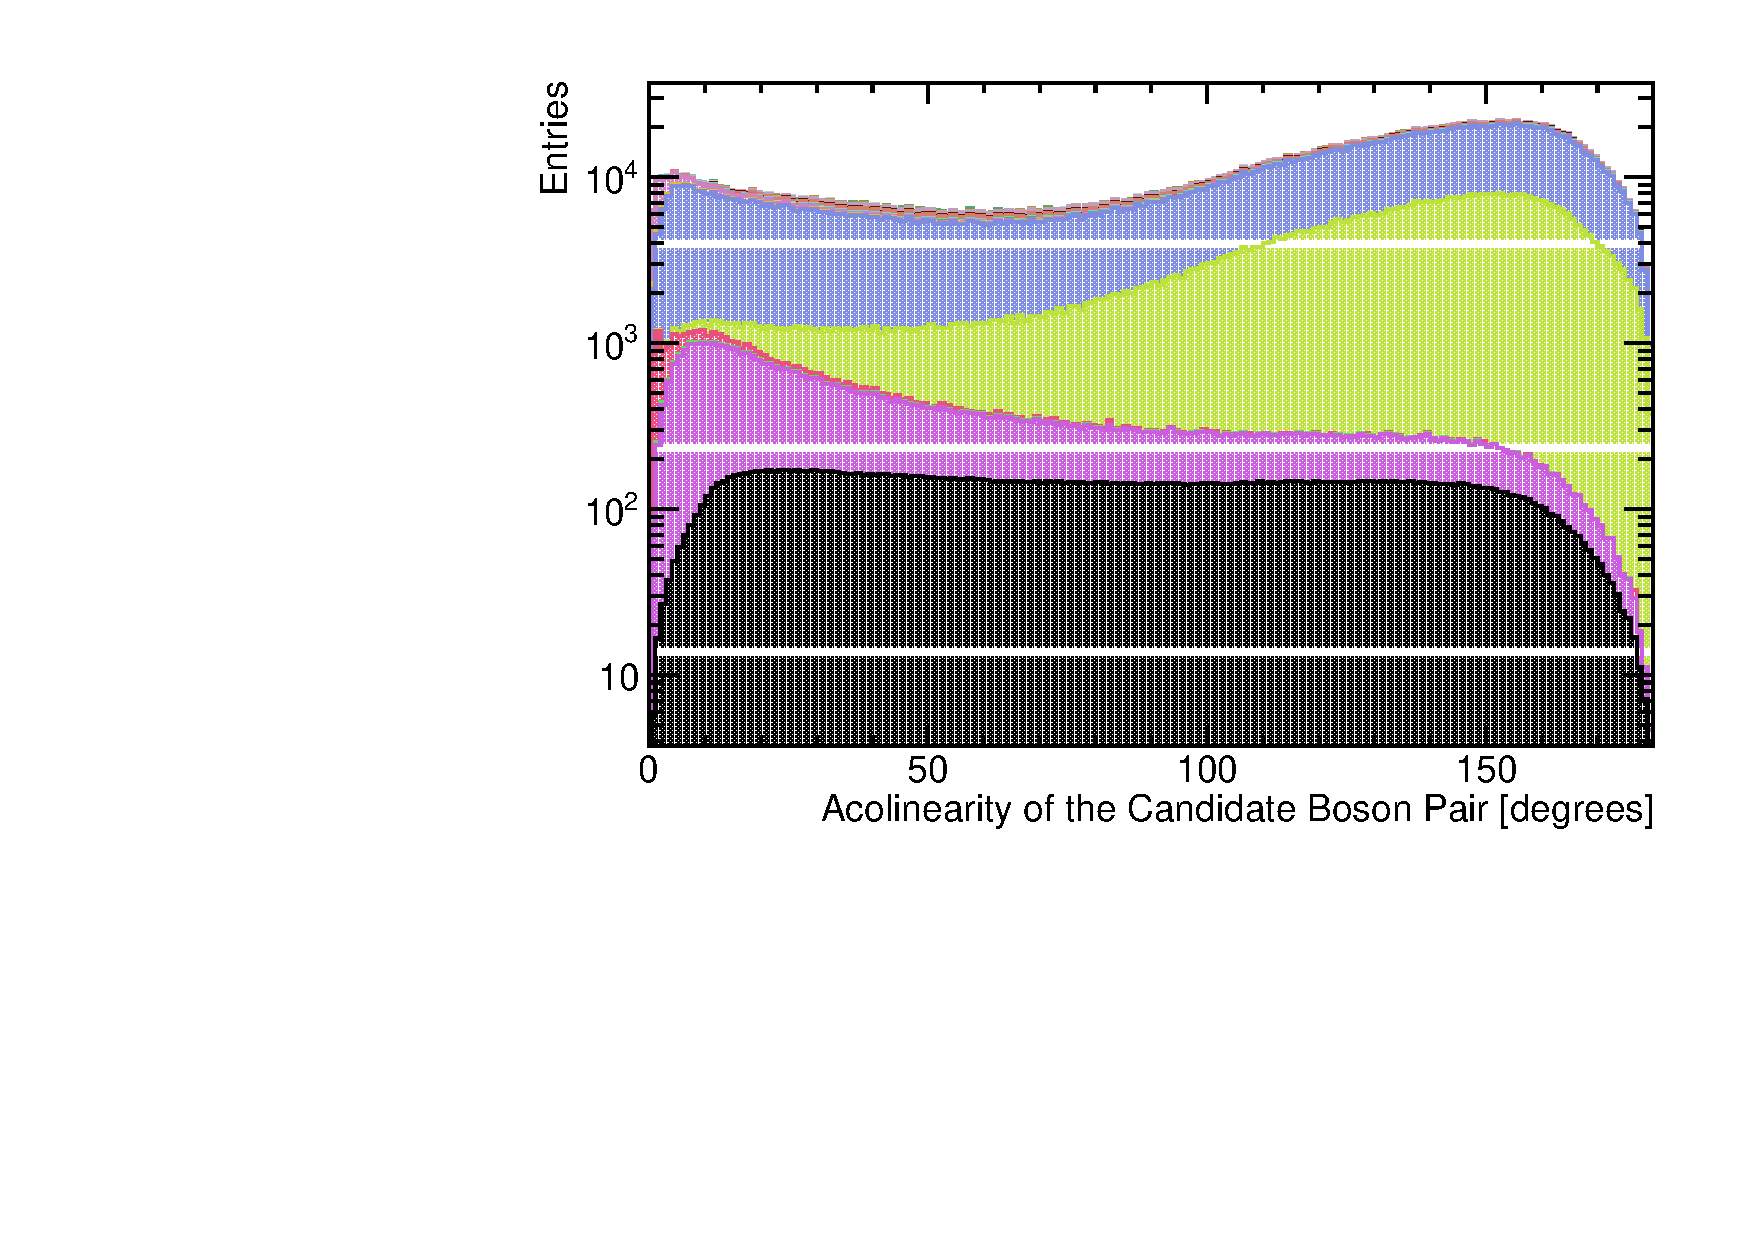
\includegraphics[width=0.5\textwidth]{PhysicsAnalysis/Plots/HighRankingVariables/1400GeV/AcolinearitySynBosons_1400GeV_Pt_gt100GeV_NIsoLep_eq0_Cuts_StackPlot.pdf}} \hfill
\subfloat[]{\label{fig:ranking3}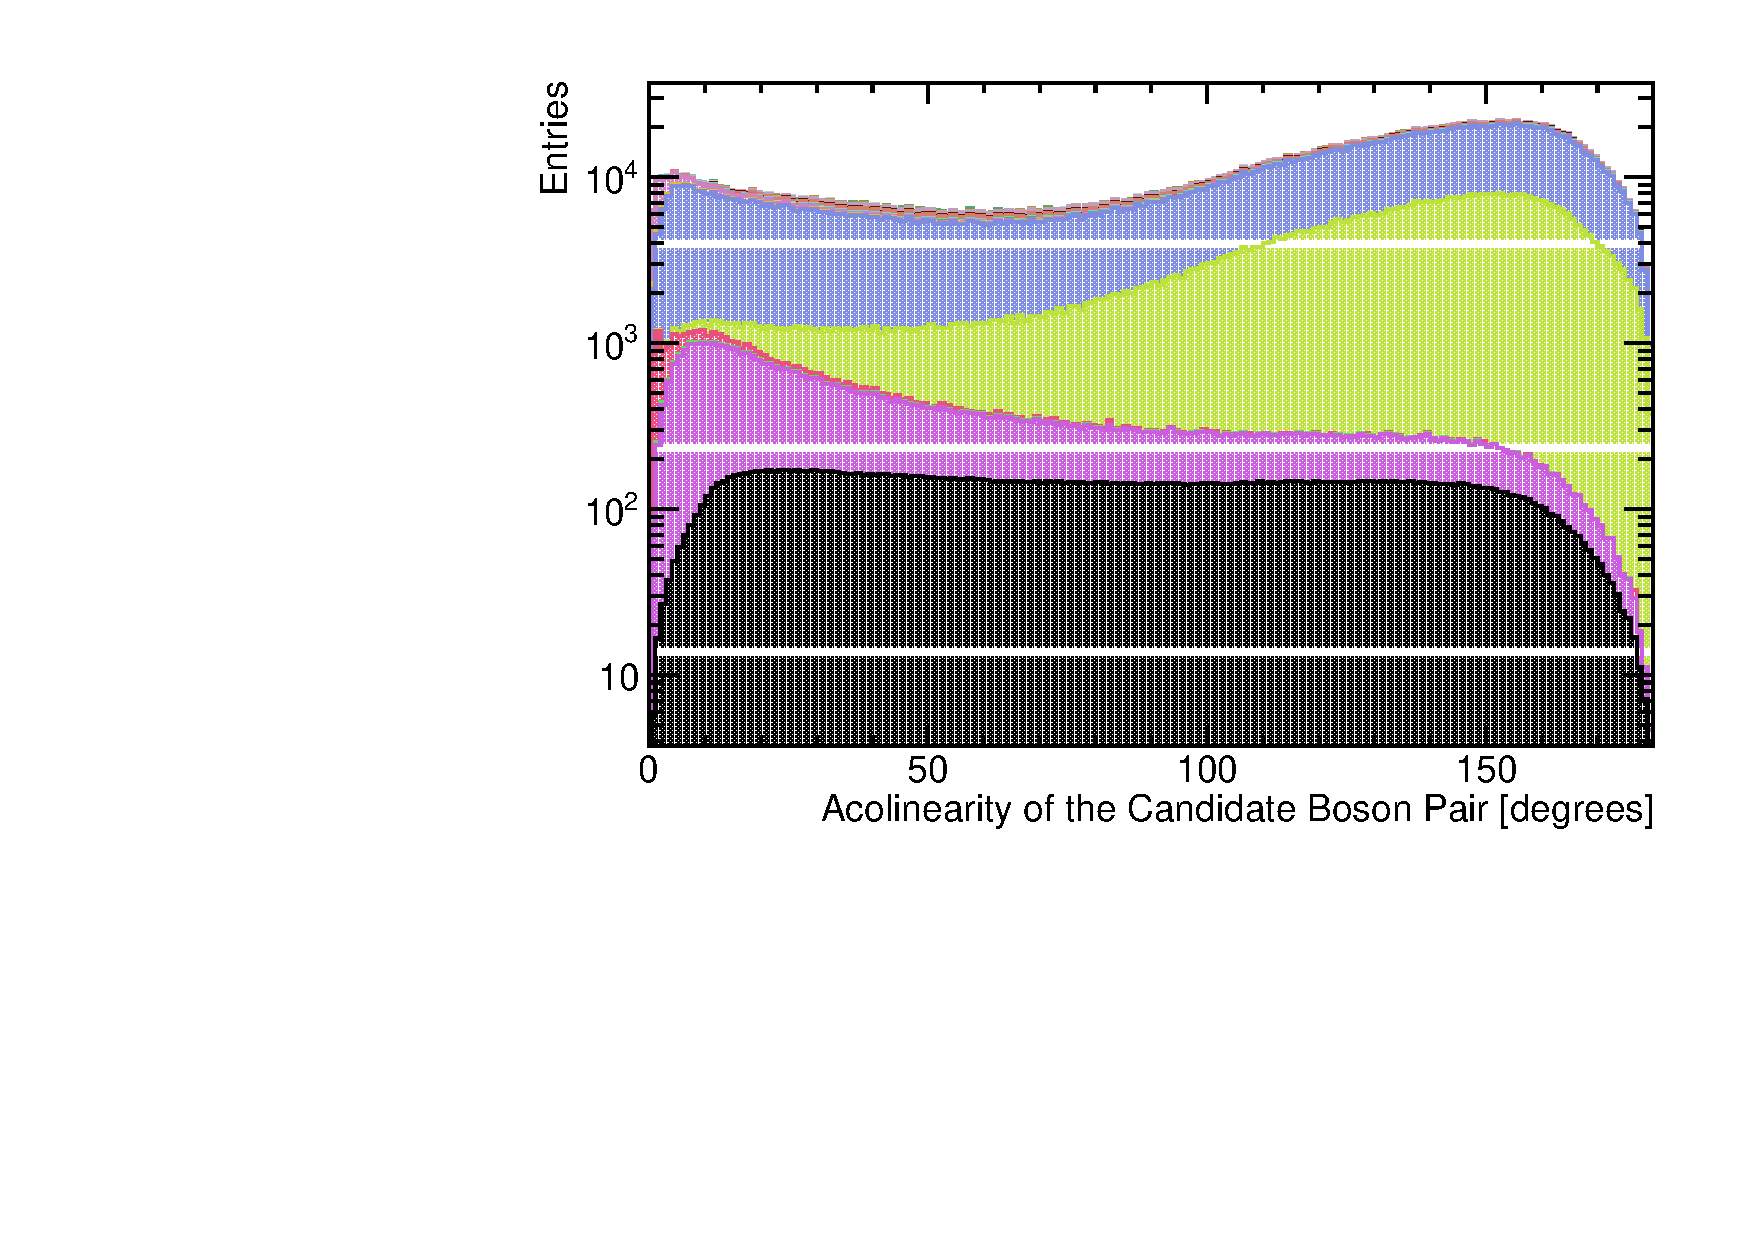
\includegraphics[width=0.5\textwidth]{PhysicsAnalysis/Plots/HighRankingVariables/1400GeV/AcolinearitySynBosons_1400GeV_Pt_gt100GeV_NIsoLep_eq0_Cuts_StackPlot.pdf}} 
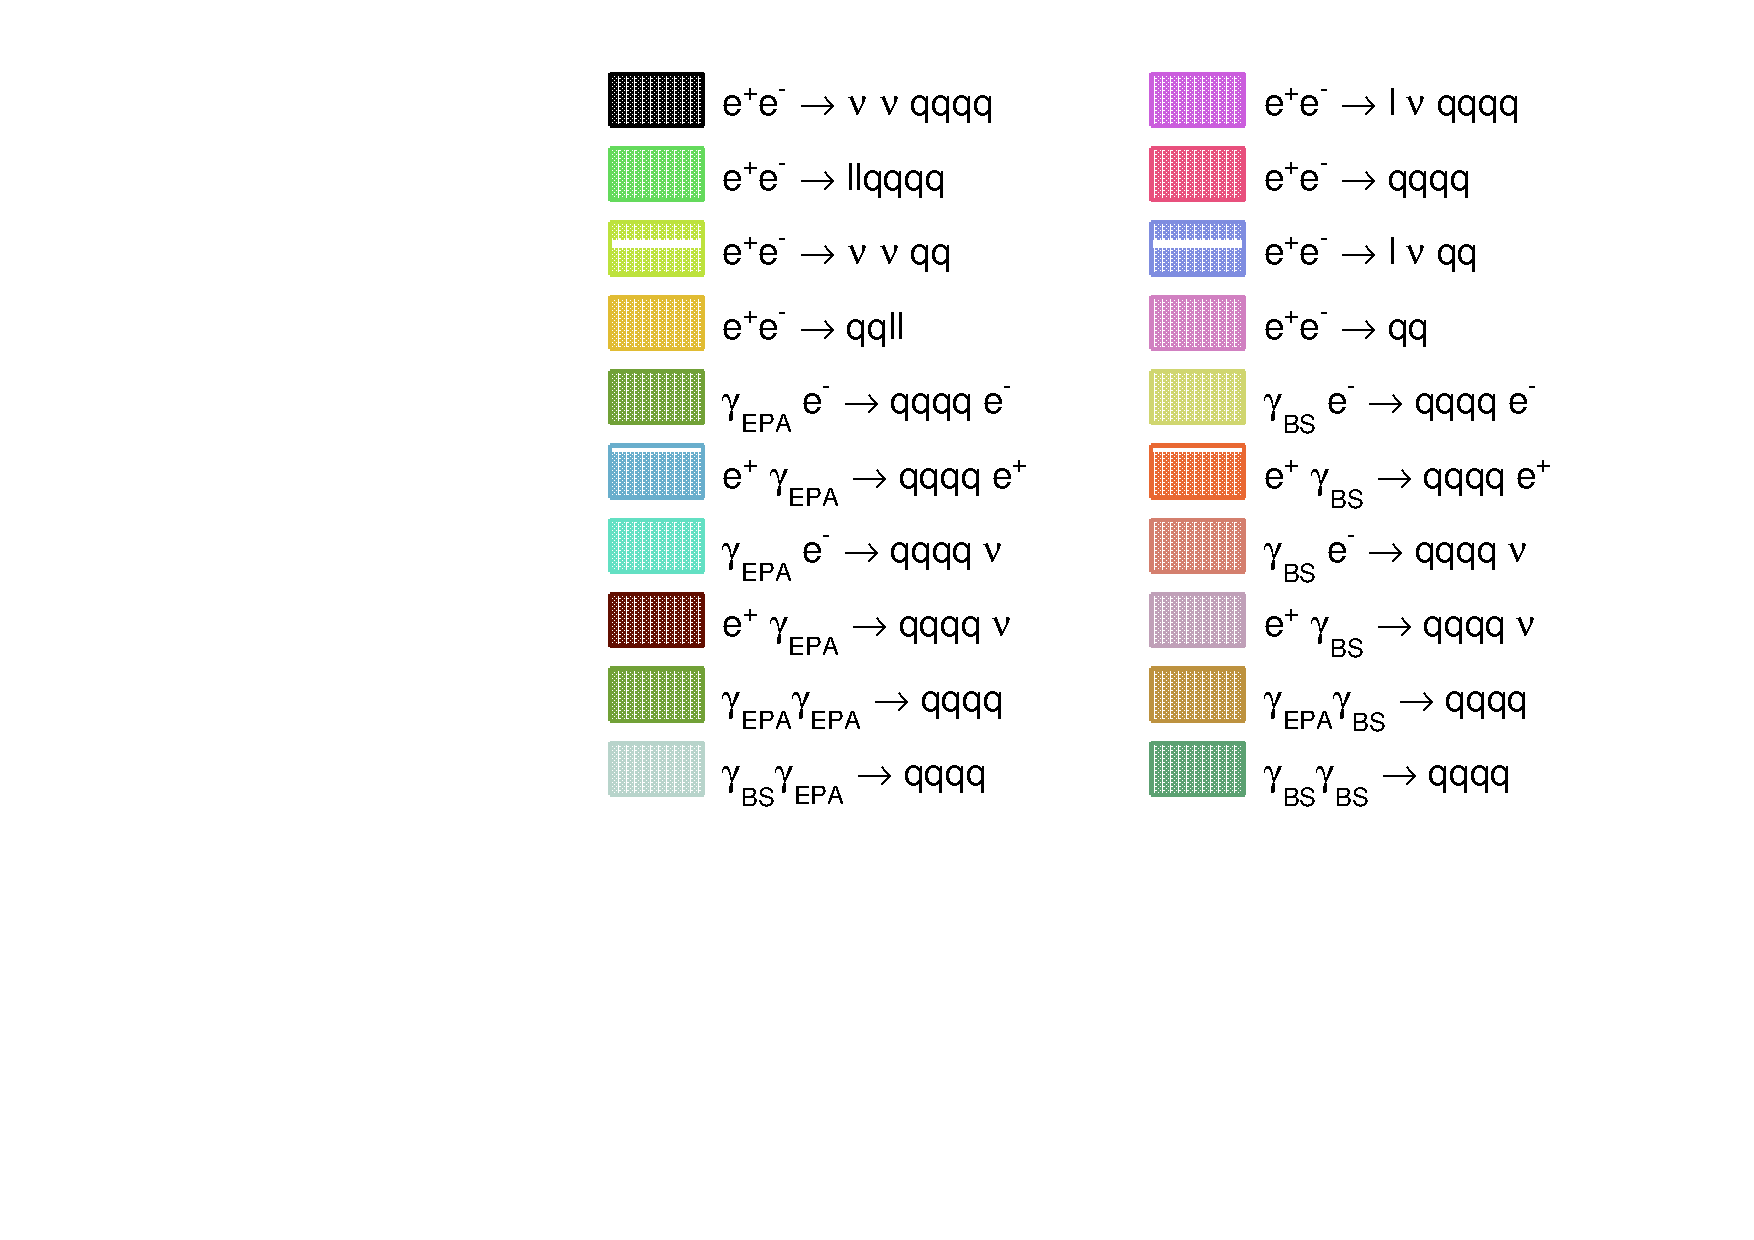
\includegraphics[width=0.5\textwidth]{PhysicsAnalysis/Plots/PreSelection/1400GeV/Legend.pdf}
\caption[Distributions of the highest ranked variables used by the BDT: \protect\subref{fig:ranking1} the acolinearity of the candidate boson pair; \protect\subref{fig:ranking2} the invariant mass of the highest energy candidate boson; and \protect\subref{fig:ranking3} the number of particles in the highest energy jet.  All distributions are normalised to an integrated luminosity of $\mathcal{L}_{int} = 1.5\text{ ab}^{-1}$.]{\textcolor{blue}{Distributions of the highest ranked variables used by the BDT: \protect\subref{fig:ranking1} the acolinearity of the candidate boson pair; \protect\subref{fig:ranking2} the invariant mass of the highest energy candidate boson; and \protect\subref{fig:ranking3} the number of particles in the highest energy jet.  All distributions are normalised to an integrated luminosity of $\mathcal{L}_{int} = 1.5\text{ ab}^{-1}$.}}
\label{fig:rankingvariables}
\end{figure}

%========================================================================================

\subsection{Event Selection Summary}
\label{sec:eventselsummary1400GeV}
The event selection is summarised using the distribution of the invariant mass of the candidate bosons, which for the signal final state should peak around the W mass.  This distribution is shown in figure \ref{fig:synbosonmass1400GeVMVAimpact} with: no event selection; with the preselection cuts applied; and with both preselections cuts and MVA applied.  The event selection efficiencies are also summarised in table \ref{table:selectionsummary1400GeV}.

As expected the dominant background processes after the MVA is applied are those that have the same topology as the signal process, i.e. four primary quarks with missing energy.  Two smaller sources of background are also present: two jet events with missing energy that are confused with four jet events with missing energy and events where a lepton is not properly reconstructed causing the event to look like four jets and missing energy.  

\begin{figure}
\centering
\subfloat[]{\label{fig:nocutssynbosonmass1400GeVMVAimpact}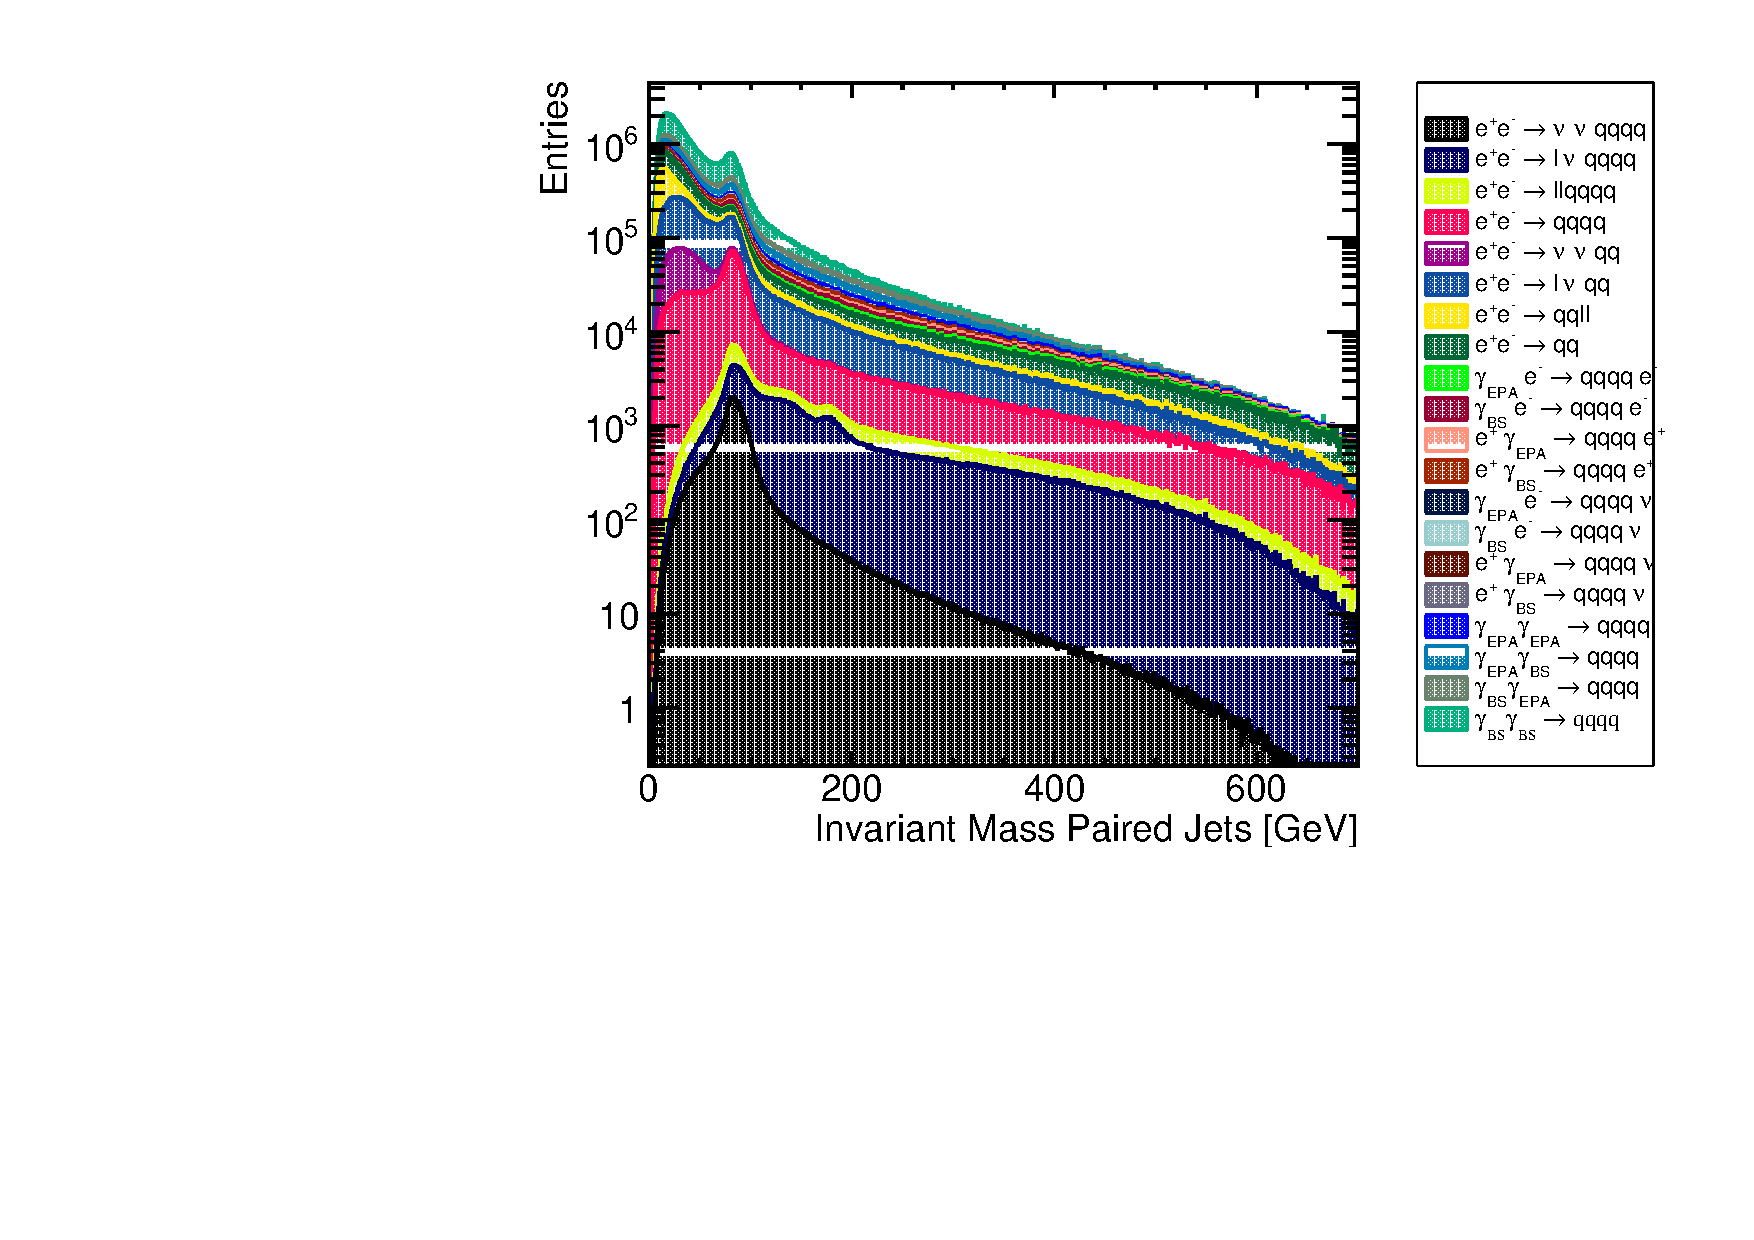
\includegraphics[width=0.5\textwidth]{PhysicsAnalysis/Plots/PostMVASelection/1400GeV/InvariantMassSynBosons_1400GeV_No_Cuts_StackPlot.pdf}}
\subfloat[]{\label{fig:postpresynbosonmass1400GeVMVAimpact}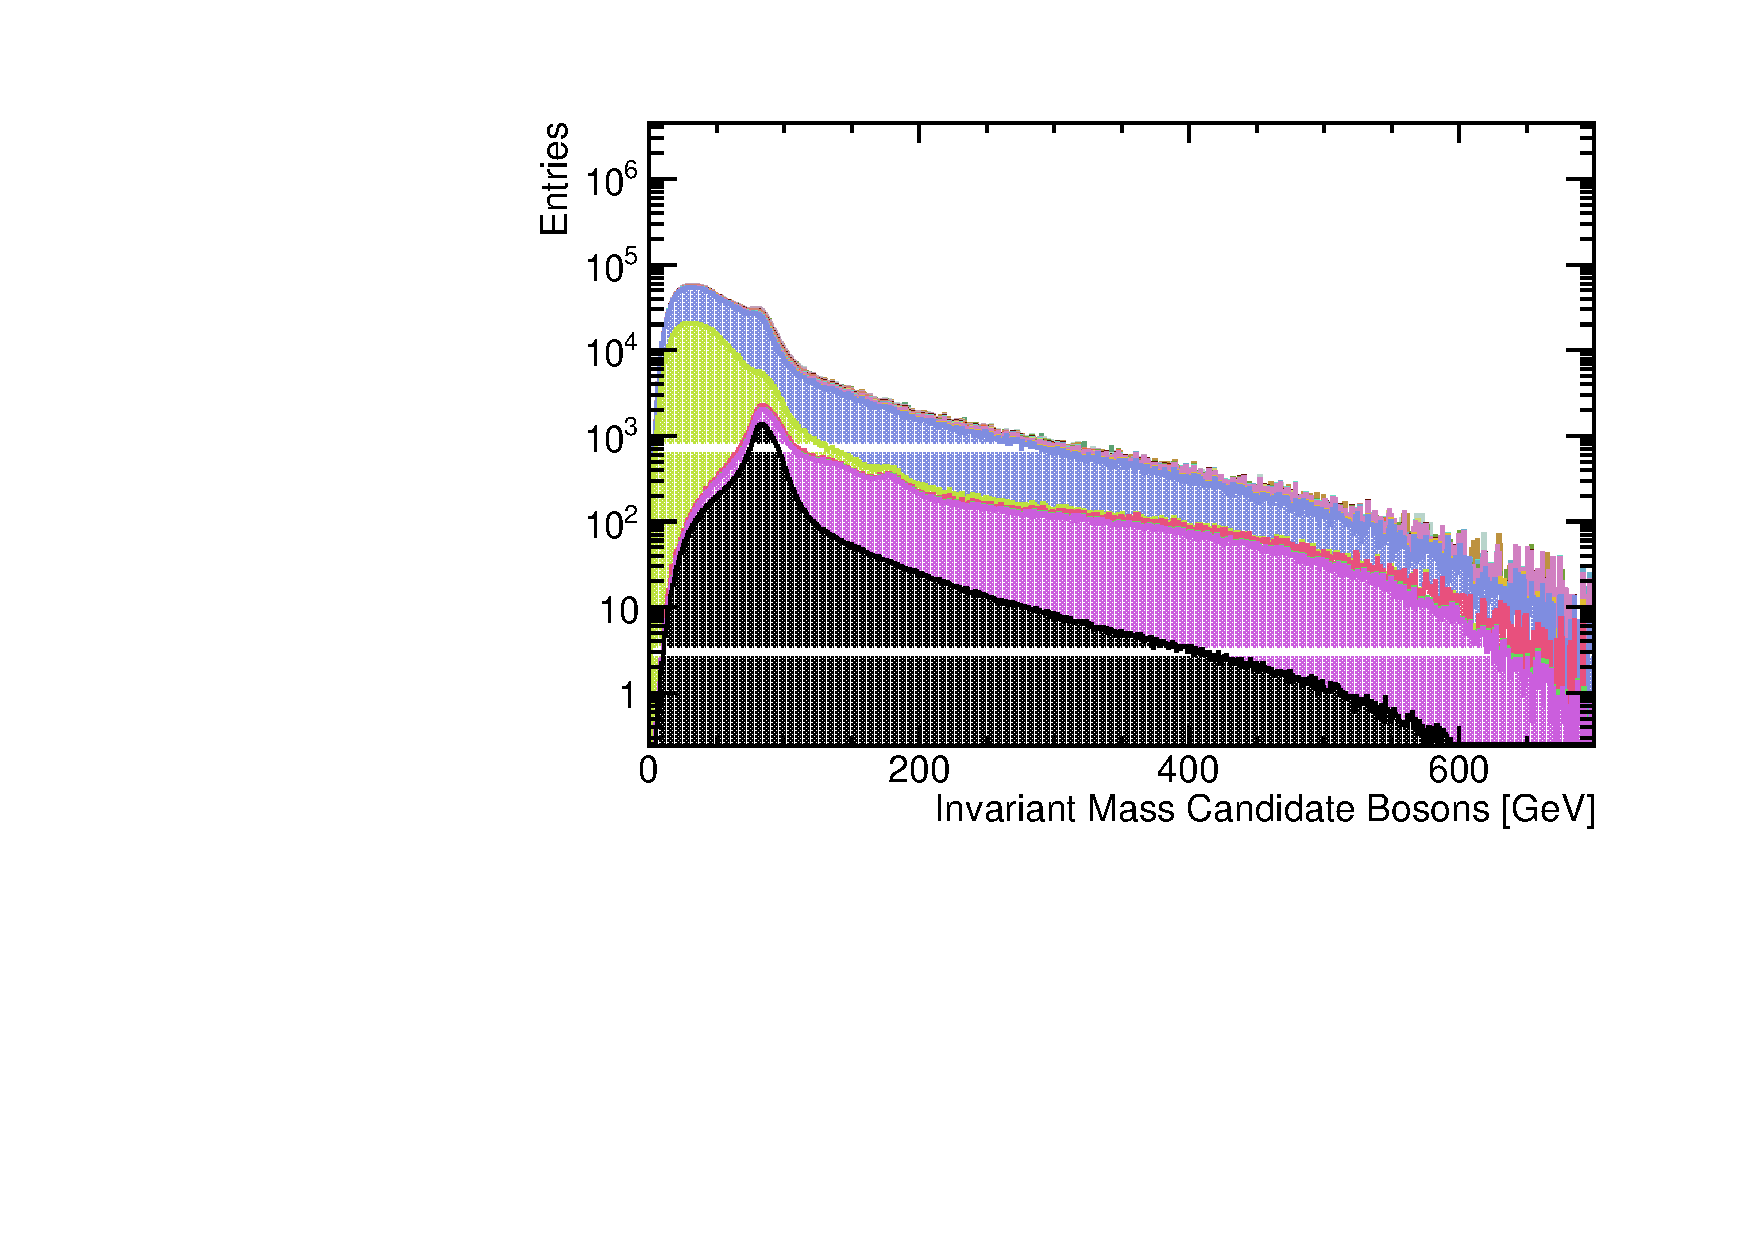
\includegraphics[width=0.5\textwidth]{PhysicsAnalysis/Plots/PostMVASelection/1400GeV/InvariantMassSynBosons_1400GeV_Pt_gt100GeV_NIsoLep_eq0_Cuts_StackPlot.pdf}}\hfill
\subfloat[]{\label{fig:postmvasynbosonmass1400GeVMVAimpact}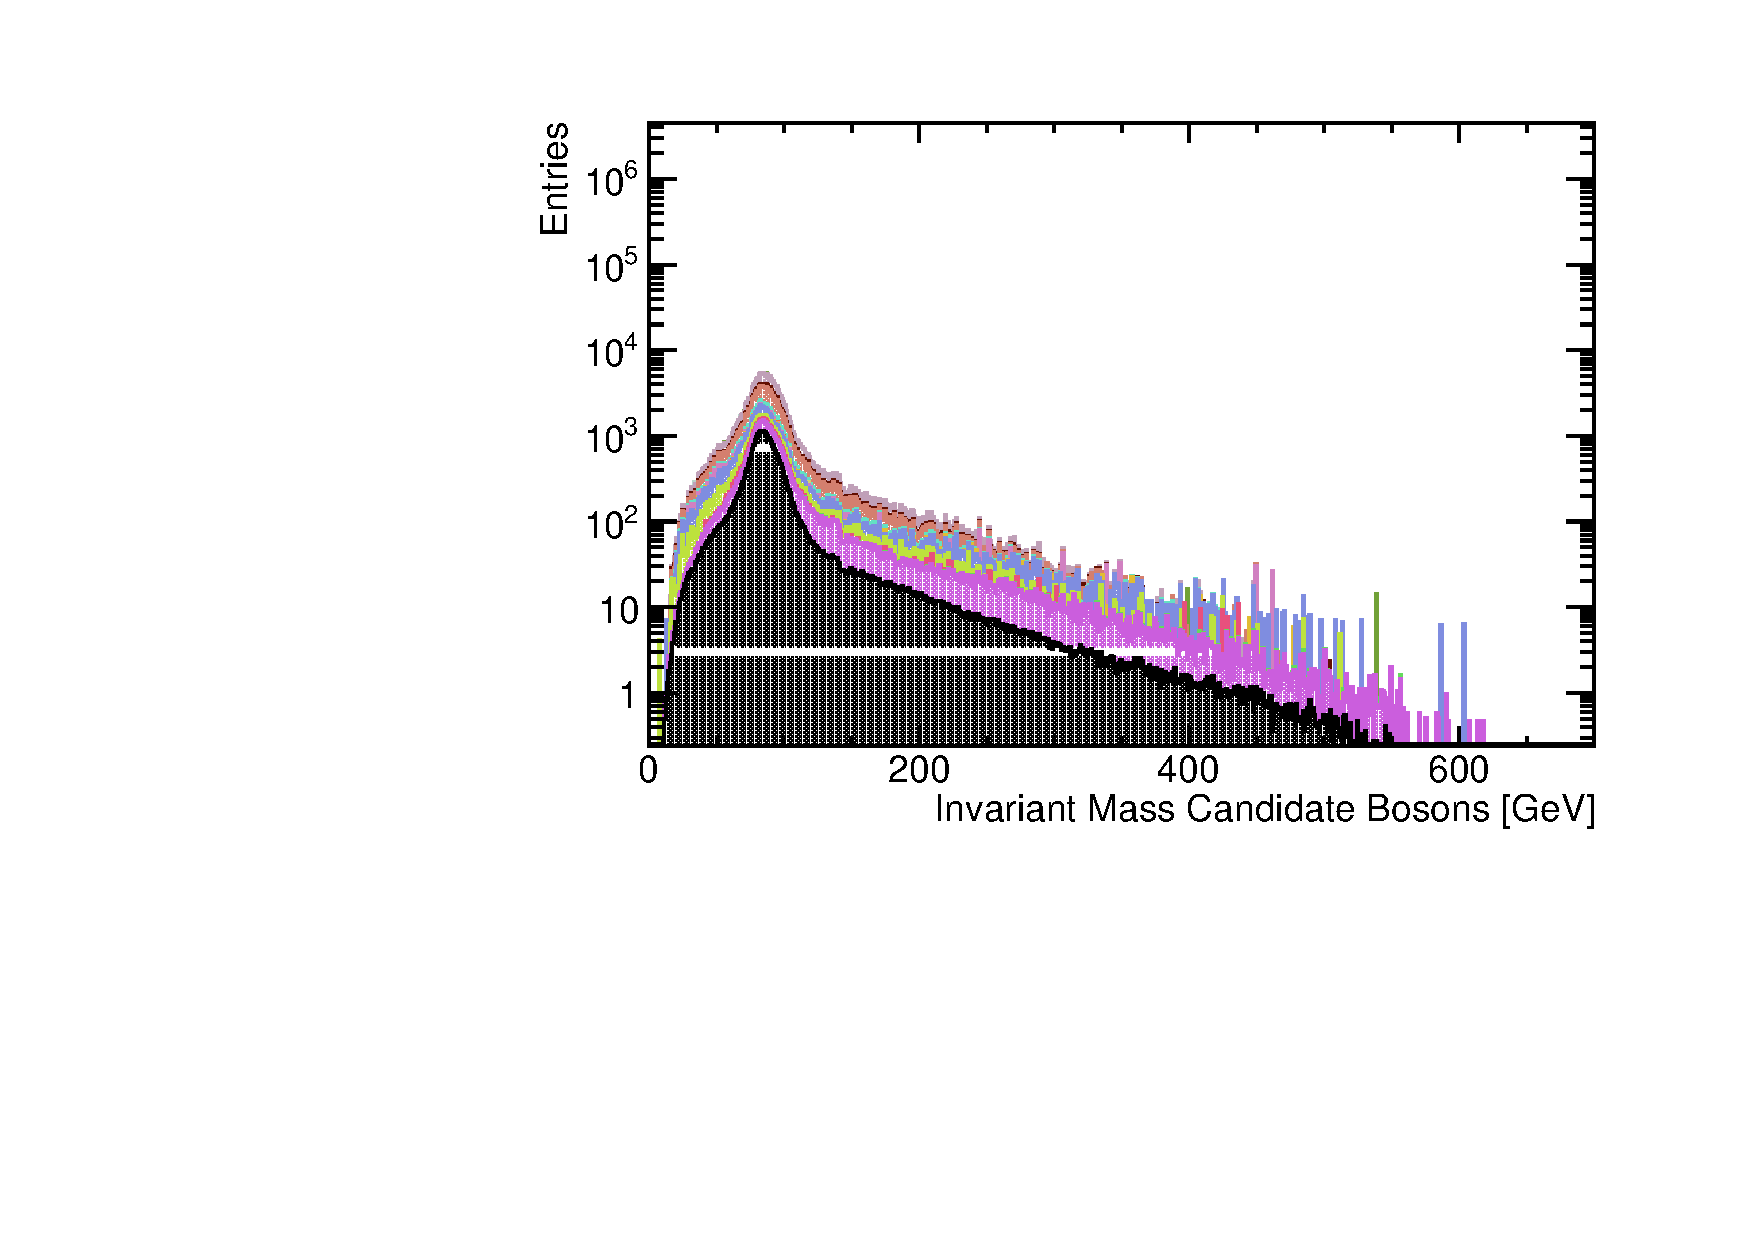
\includegraphics[width=0.5\textwidth]{PhysicsAnalysis/Plots/PostMVASelection/1400GeV/InvariantMassSynBosons_1400GeV_PostPreSelection_PostMVA_Cuts_StackPlot.pdf}} 
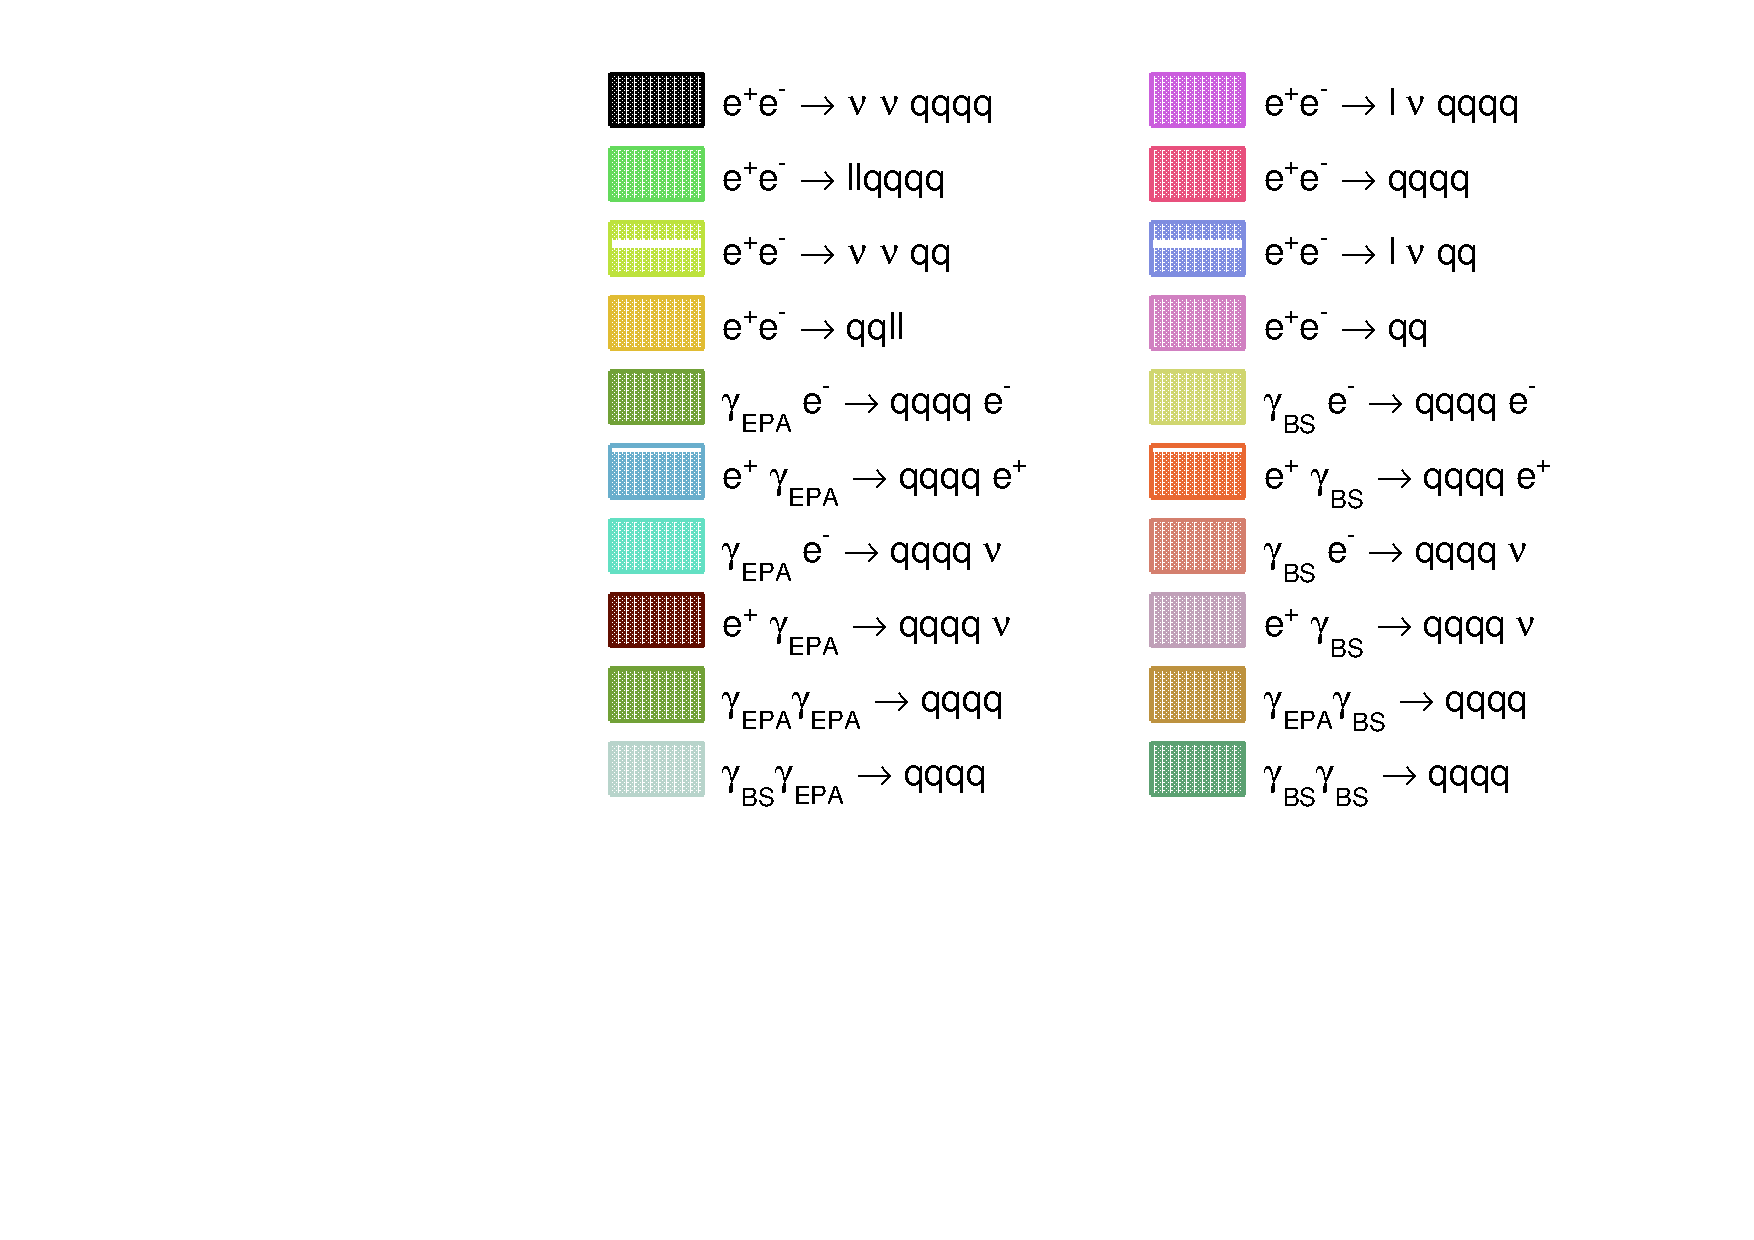
\includegraphics[width=0.5\textwidth]{PhysicsAnalysis/Plots/PreSelection/1400GeV/Legend.pdf}
\caption[Impact of preselection and MVA on the reconstructed invariant mass of the candidate bosons at $\sqrt{s}=1.4$~TeV:   \protect\subref{fig:nocutssynbosonmass1400GeVMVAimpact} no cuts; \protect\subref{fig:postpresynbosonmass1400GeVMVAimpact} after preselection; and \protect\subref{fig:postmvasynbosonmass1400GeVMVAimpact} after preselection and MVA.  All distributions correspond to an integrated luminosity of $\mathcal{L}_{int} = 1.5\text{ ab}^{-1}$.]{Impact of preselection and MVA on the reconstructed invariant mass of the candidate bosons at $\sqrt{s}=1.4$~TeV:   \protect\subref{fig:nocutssynbosonmass1400GeVMVAimpact} no cuts; \protect\subref{fig:postpresynbosonmass1400GeVMVAimpact} after preselection; and \protect\subref{fig:postmvasynbosonmass1400GeVMVAimpact} after preselection and MVA.  All distributions correspond to an integrated luminosity of $\mathcal{L}_{int} = 1.5\text{ ab}^{-1}$.}
\label{fig:synbosonmass1400GeVMVAimpact}
\end{figure}

\begin{table}[h!]
\centering
\begin{tabular}{ l r r r }
\hline
Final State & $\epsilon_{\text{presel}}$ & $\epsilon_{\text{BDT}}$ & $N_{\text{BDT}}$ \\ 
\hline
$\text{e}^{+}\text{e}^{-} \rightarrow \nu{\nu}\text{qqqq}$ & 64.1\% & 44.5\% & 16,470 \\
$\text{e}^{+}\text{e}^{-} \rightarrow \nu\text{lqqqq}$ & 26.1\% & 5.2\% & 8,582 \\
$\text{e}^{+}\text{e}^{-} \rightarrow \text{llqqqq}$ & 0.8\% & 0.1\% & 100 \\
$\text{e}^{+}\text{e}^{-} \rightarrow \text{qqqq}$ & 0.3\% & 0.1\% & 1,698 \\
$\text{e}^{+}\text{e}^{-} \rightarrow \nu{\nu}\text{qq}$ & 43.4\% & 0.5\% & 5,351 \\
$\text{e}^{+}\text{e}^{-} \rightarrow \nu\text{lqq}$ & 19.1\% & 0.1\% & 9,319 \\
$\text{e}^{+}\text{e}^{-} \rightarrow \text{llqq}$ & 0.1\% & - & 234 \\
$\text{e}^{+}\text{e}^{-} \rightarrow \text{qq}$ & 0.6\% & - & 1,586 \\
$\text{e}^{-}\gamma_{\text{EPA}} \rightarrow \text{e}^{-}\text{qqqq}$ & 0.2\% & - & 48 \\
$\text{e}^{-}\gamma_{\text{BS}} \rightarrow \text{e}^{-}\text{qqqq}$ & 0.1\% & - & 42 \\
$\text{e}^{+}\gamma_{\text{EPA}} \rightarrow \text{e}^{+}\text{qqqq}$ & 0.3\% & - & 19 \\
$\text{e}^{+}\gamma_{\text{BS}} \rightarrow \text{e}^{+}\text{qqqq}$ & - & - & 65 \\
$\text{e}^{-}\gamma_{\text{EPA}} \rightarrow \nu_{\text{e}}\text{qqqq}$ & 26.0\% & 9.0\% & 4,421 \\
$\text{e}^{-}\gamma_{\text{BS}} \rightarrow \nu_{\text{e}}\text{qqqq}$ & 36.1\% & 15.0\% & 23,150 \\
$\text{e}^{+}\gamma_{\text{EPA}} \rightarrow \overline{\nu}_{\text{e}}\text{qqqq}$ & 25.9\% & 9.2\% & 4,495 \\
$\text{e}^{+}\gamma_{\text{BS}} \rightarrow \overline{\nu}_{\text{e}}\text{qqqq}$ & 36.4\% & 15.3\% & 23,410 \\
$\gamma_{\text{EPA}}\gamma_{\text{EPA}} \rightarrow \text{qqqq}$ & 0.2\% & - & 81 \\
$\gamma_{\text{EPA}}\gamma_{\text{BS}} \rightarrow \text{qqqq}$ & 0.1\% & - & 55 \\
$\gamma_{\text{BS}}\gamma_{\text{EPA}} \rightarrow \text{qqqq}$ & - & - & 53 \\
$\gamma_{\text{BS}}\gamma_{\text{BS}} \rightarrow \text{qqqq}$ & - & - & 0 \\
\hline
\end{tabular}
\caption[Event selection efficiencies at $\sqrt{s}=1.4$~TeV.  In the above table, $\epsilon_{presel}$ denotes the number of events passing the preselection as a fraction of the total number of events, while $\epsilon_{BDT}$ denotes the number of events passing both the preselection and the BDT as a fraction of the total number of events.  The EPA and BS subscript on the incoming photon indicates whether the photon is generated from the equivalent photon approximation or beamstrahlung.  Entries with a dash indicate an efficiency of less than 0.1\%.  The event numbers correspond to an integrated luminosity of $\mathcal{L}_{int} = 1.5\text{ ab}^{-1}$.]{Event selection efficiencies at $\sqrt{s}=1.4$~TeV.  In the above table, $\epsilon_{presel}$ denotes the number of events passing the preselection as a fraction of the total number of events, while $\epsilon_{BDT}$ denotes the number of events passing both the preselection and the BDT as a fraction of the total number of events.  The EPA and BS subscript on the incoming photon indicates whether the photon is generated from the equivalent photon approximation or beamstrahlung.  Entries with a dash indicate an efficiency of less than 0.1\%.  The event numbers correspond to an integrated luminosity of $\mathcal{L}_{int} = 1.5\text{ ab}^{-1}$.}
\label{table:selectionsummary1400GeV}
\end{table}

%========================================================================================
%========================================================================================

\section{Anomalous Coupling Fitting Methodology}
\label{sec:fitting}
This section describes the procedure used for constructing the $\chi^{2}$ surface and the subsequent confidence contours used to determine the sensitivity of CLIC to the anomalous gauge couplings $\alpha_{4}$ and $\alpha_{5}$.

%========================================================================================

\subsection{Sensitive Distribution}
The sensitivity of CLIC to the anomalous gauge couplings will be determined through the use of a $\chi^{2}$ fit.  Three variables showing sensitivity to the anomalous gauge couplings were considered for use in the $\chi^{2}$ fit:
\begin{itemize}
\item \textbf{$M_{VV}$}.  The invariant mass of the visible system;
\item \textbf{$\text{cos}\theta^{*}_{Bosons}$}.  The angle between the boost direction and the back-to-back candidate bosons in the rest frame of the visible system;
\item \textbf{$\text{cos}\theta^{*}_{Jets}$}.  The angle between the boost direction and the back-to-back jets in the rest frame of the candidate bosons.  As each event contains two candidate bosons, there are two $\text{cos}\theta^{*}_{Jets}$ variables per event. 
\end{itemize}

Figure \ref{fig:variables} shows the distribution of these variables for the  \nu{\nu}qqqq final state for selected values of the anomalous gauge couplings $\alpha_{4}$ and $\alpha_{5}$.  A $\chi^{2}$ fit to each of these variables was applied to obtain confidence limits on the sensitivity of CLIC to the anomalous gauge couplings, as described in section \ref{sec:chi2surfacedefinition}.  The distributions used for the $\chi^{2}$ fit contained signal and background events that passed event selection.  Table \ref{table:sensitivevariables} shows the 68\% confidence limits on the measurement of $\alpha_{4}$ and $\alpha_{5}$ obtained using each of the variables considered.  The $M_{VV}$ distribution shows the greatest sensitive to the anomalous gauge couplings; therefore, it will be used by all subsequent $\chi^{2}$ fits when reporting sensitivities.  This distribution shows the greatest sensitivity of the variables considered because the couplings primarily affect events with large values of $M_{VV}$ and there are relatively few of these events.    

\begin{figure}[h!]
\subfloat[]{\label{fig:mvv1400GeV} 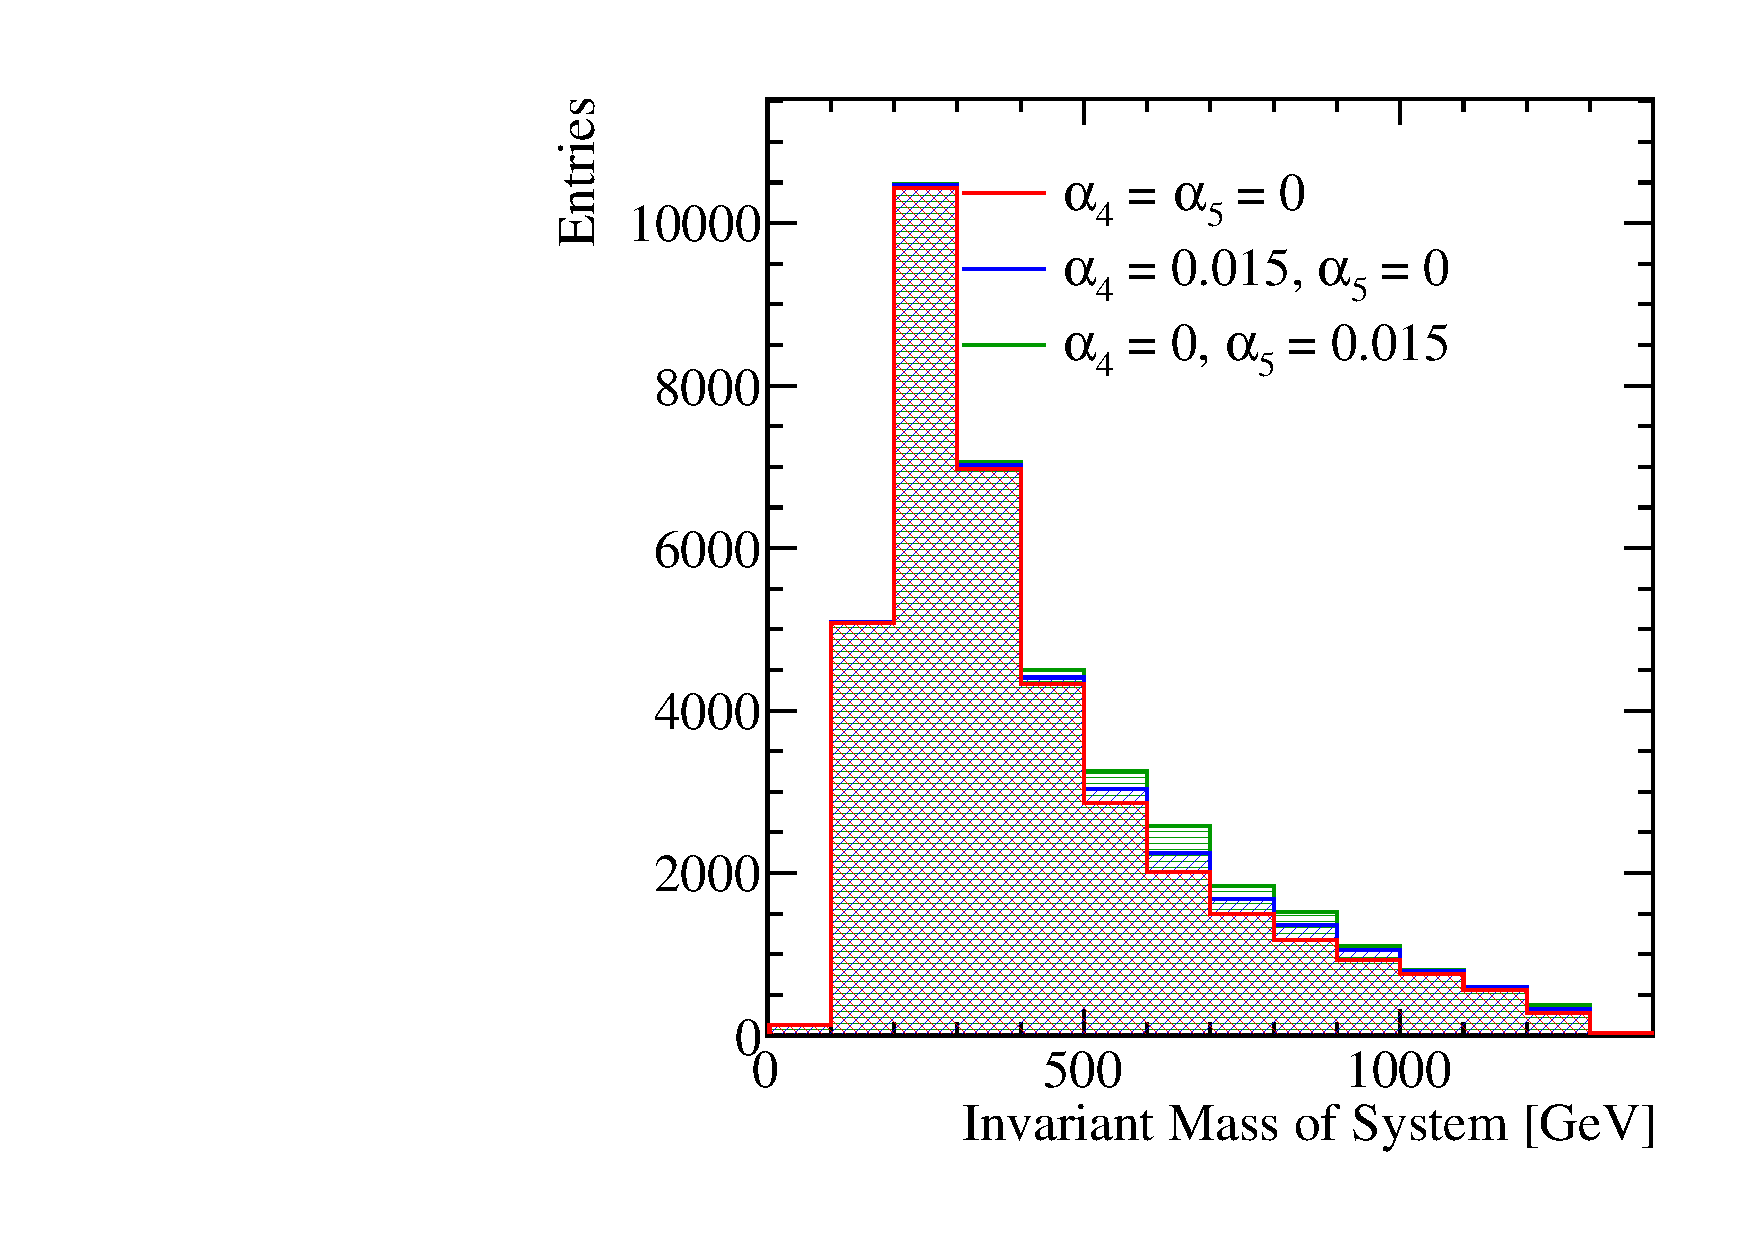
\includegraphics[width=0.5\textwidth]{PhysicsAnalysis/Plots/SensitiveDistributions/MVVs_SPFOs_kt_0p90_1400GeV.pdf}}
\subfloat[]{\label{fig:costhetastarjets1400GeV} 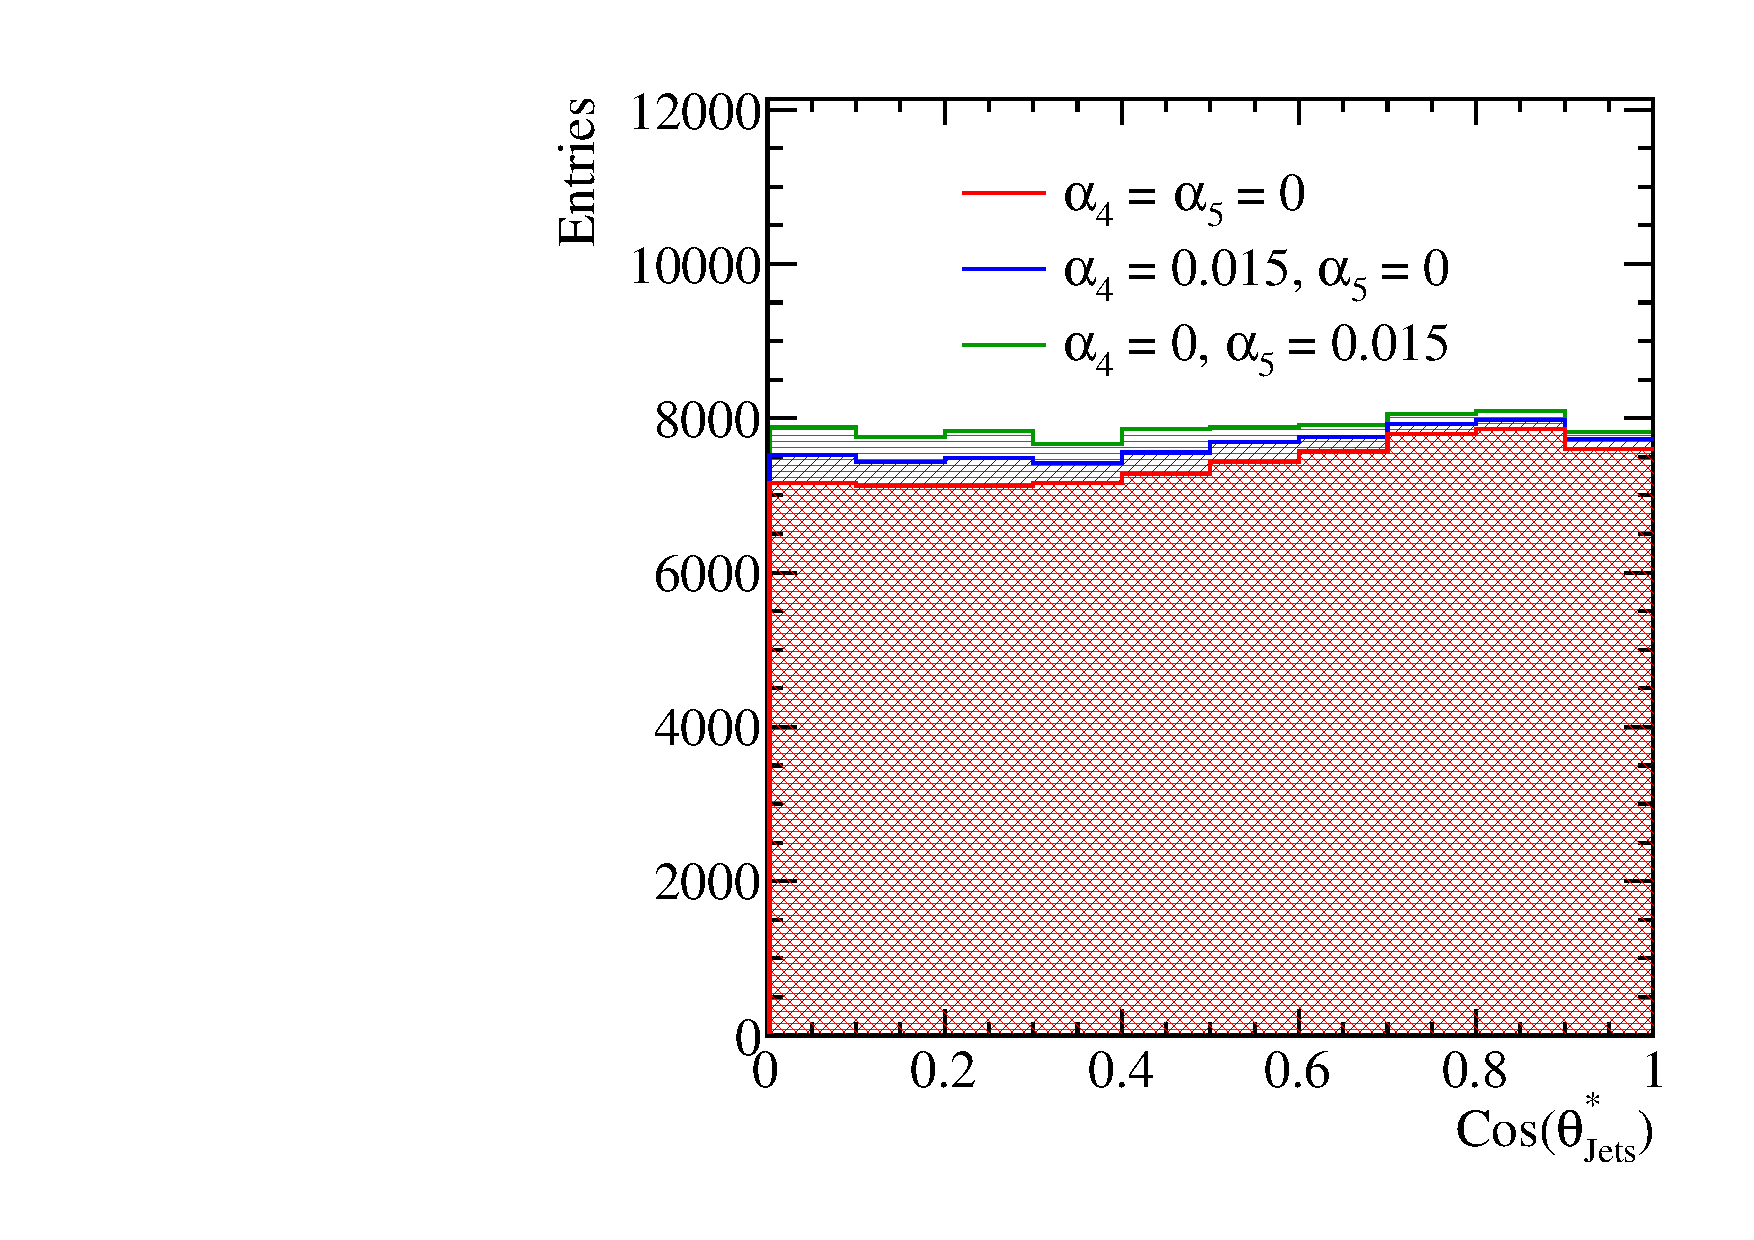
\includegraphics[width=0.5\textwidth]{PhysicsAnalysis/Plots/SensitiveDistributions/CosThetaStarSynJets_SPFOs_kt_0p90_1400GeV.pdf}} \\
\subfloat[]{\label{fig:costhetastarbosons1400GeV} 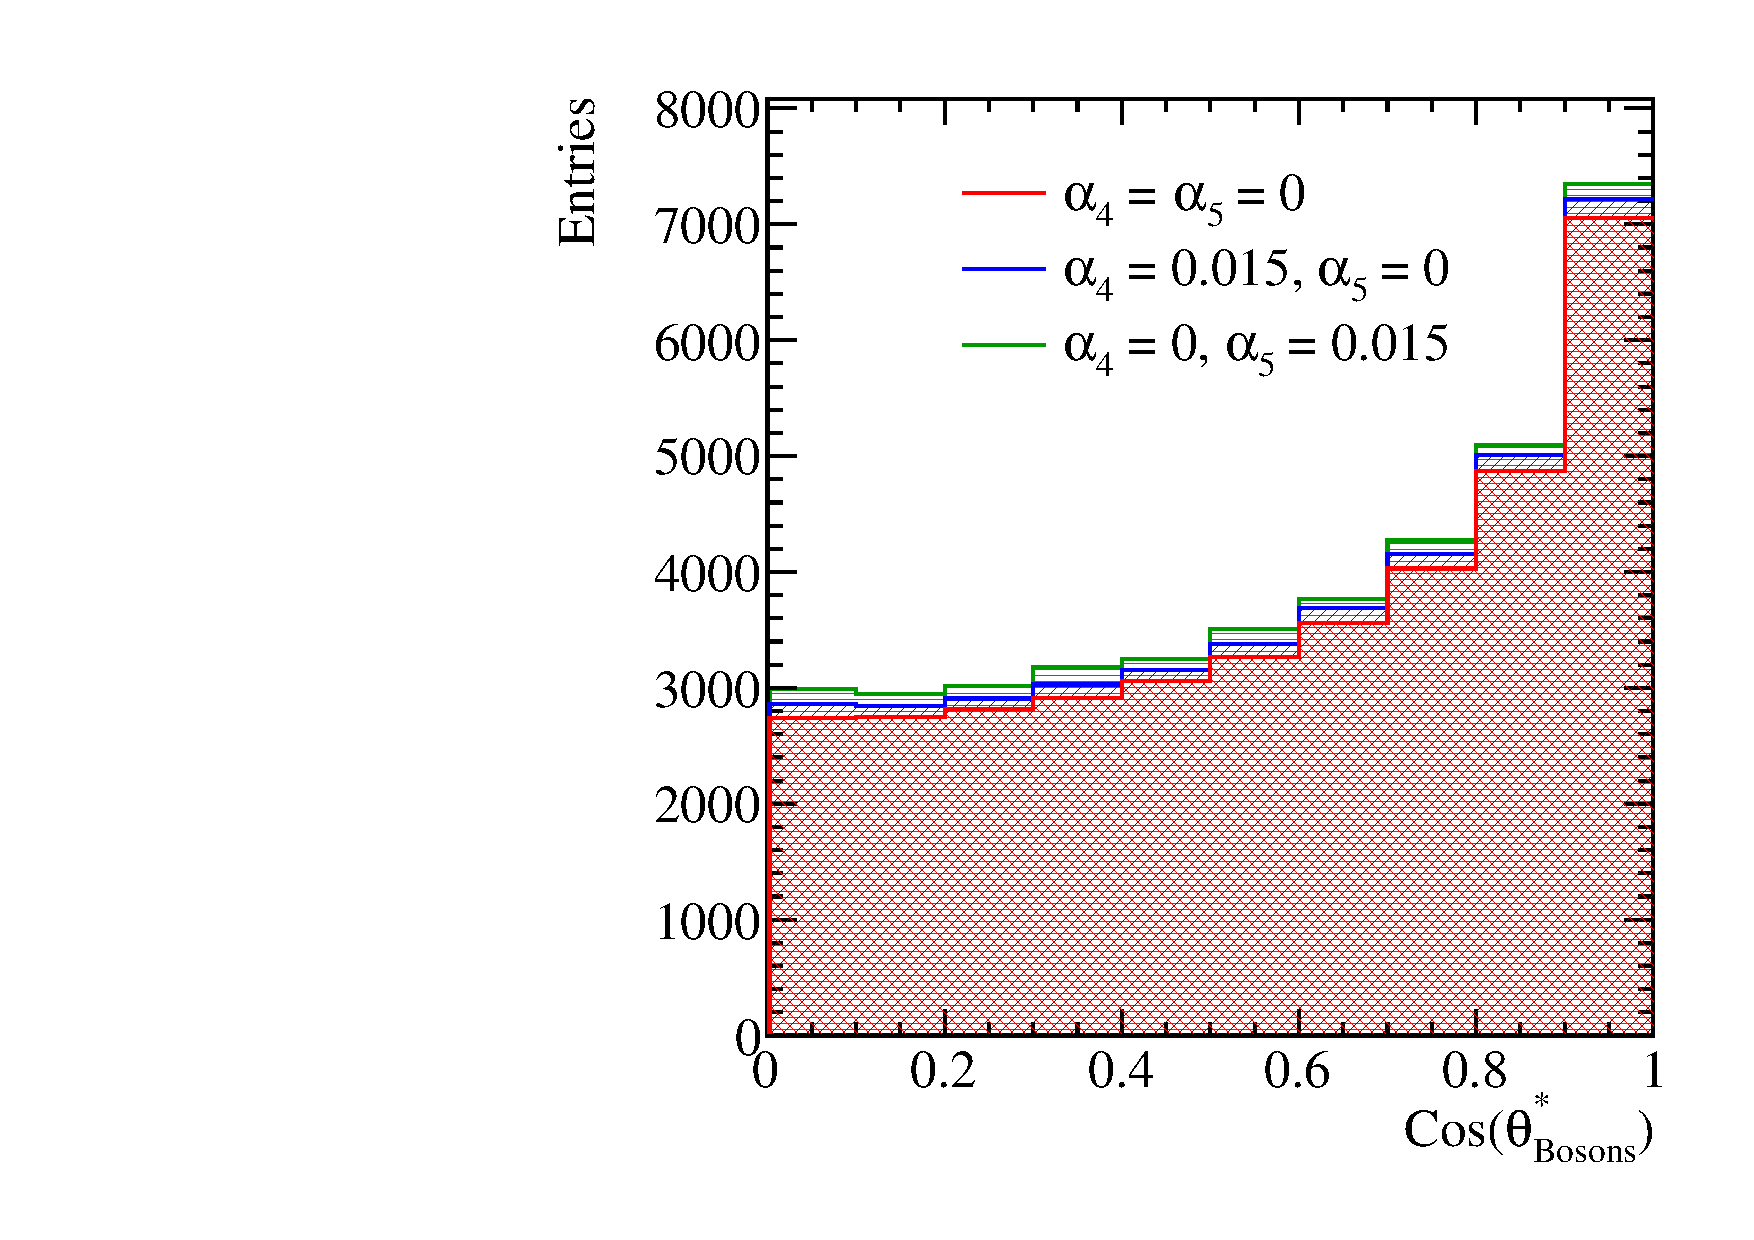
\includegraphics[width=0.5\textwidth]{PhysicsAnalysis/Plots/SensitiveDistributions/CosThetaStarSynBosons_SPFOs_kt_0p90_1400GeV.pdf}}
\caption[The distributions of \protect\subref{fig:mvv1400GeV} $M_{VV}$, \protect\subref{fig:costhetastarjets1400GeV} $\text{cos}\theta^{*}_{Jets}$ and \protect\subref{fig:costhetastarbosons1400GeV} $\text{cos}\theta^{*}_{Bosons}$ for selected values of the anomalous gauge couplings $\alpha_{4}$ and $\alpha_{5}$ for the \nu{\nu}qqqq final state at $\sqrt{s}=1.4$~TeV.  The jet algorithm used was the longitudinally invariant $k_{t}$ algorithm with an R parameter of 0.9 and Selected PFOs.  All distributions are normalised to an integrated luminosity of $\mathcal{L}_{int} = 1.5\text{ ab}^{-1}$.]{The distributions of \protect\subref{fig:mvv1400GeV} $M_{VV}$, \protect\subref{fig:costhetastarjets1400GeV} $\text{cos}\theta^{*}_{Jets}$ and \protect\subref{fig:costhetastarbosons1400GeV} $\text{cos}\theta^{*}_{Bosons}$ for selected values of the anomalous gauge couplings $\alpha_{4}$ and $\alpha_{5}$ for the \nu{\nu}qqqq final state at $\sqrt{s}=1.4$~TeV.  The jet algorithm used was the longitudinally invariant $k_{t}$ algorithm with an R parameter of 0.9 and Selected PFOs.  All distributions are normalised to an integrated luminosity of $\mathcal{L}_{int} = 1.5\text{ ab}^{-1}$.}
\label{fig:variables}
\end{figure}

\begin{table}[h!]
\centering
\begin{tabular}{l l l l}
\hline
Sensitive Variable & 68\% Confidence Limit \\
\hline
\multirow{ 2}{*}{$M_{VV}$} 					& $-0.0082 < \alpha_{4} < 0.0116$ \\
										& $-0.0055 < \alpha_{5} < 0.0078$ \\
\hline
\multirow{ 2}{*}{$\text{cos}\theta^{*}_{Bosons}$} 	& $-0.0111 < \alpha_{4} < 0.0155$ \\
										& $-0.0082 < \alpha_{5} < 0.0110$ \\
\hline
\multirow{ 2}{*}{$\text{cos}\theta^{*}_{Jets}$} 		& $-0.0100 < \alpha_{4} < 0.0142$ \\
										& $-0.0070 < \alpha_{5} < 0.0098$ \\
\end{tabular}
\caption[The 68\% confidence limits on the measurement of $\alpha_{4}$ and $\alpha_{5}$ obtained at $\sqrt{s} = 1.4$~TeV.  These sensitivities include the effect from backgrounds and event selection.]{The 68\% confidence limits on the measurement of $\alpha_{4}$ and $\alpha_{5}$ obtained at $\sqrt{s} = 1.4$~TeV.  These sensitivities include the effect from backgrounds and event selection.} 
\label{table:sensitivevariables}
\end{table}

%========================================================================================

\subsection{$\chi^{2}$ Surface and Confidence Limit Definition}
\label{sec:chi2surfacedefinition}
A $\chi^{2}$ surface was used to determine confidence limits on the anomalous gauge couplings given the null hypothesis that $\alpha_{4} = \alpha_{5} = 0$.  This surface is defined as  
%
\begin{equation}
\chi^{2} = \sum_{i} \frac{(O_{i} - E_{i})^{2}}{E_{i}} \text{,}
\end{equation}
%
\noindent where $O_{i}$ is the observed, $\alpha_{4} = \alpha_{5} = 0$, and $E_{i}$ the expected, $\alpha_{4} \neq 0$ and $\alpha_{5} \neq 0$, bin content for bin $i$ in the distribution of interest.  The summation $\Sigma_{i}$ runs over bins in the distribution of interest.  

When applying the $\chi^{2}$ fit to the $M_{VV}$ distribution, the distribution was binned using 13 bins as shown in figure \ref{fig:signalbackgroundfit}.  The first bin spanned the invariant mass range between 0~GeV and 200~GeV, this was followed by 11 bins of width 100~GeV ranging from 200~GeV to 1300~GeV and finally the last bin contained all invariant masses above 1300~GeV.  The expanded bin widths at the tails of the distribution were chosen to ensure the bin contents were sufficiently large to give a reliable estimate of the likelihood function using the $\chi^{2}$ parameter.  This choice of bin width also ensured the bin contents were sufficiently large to minimise fluctuations arising from individual events with large weights.  When applying the $\chi^{2}$ fit to distributions of the $\text{cos}\theta^{*}_{Bosons}$ and $\text{cos}\theta^{*}_{Jets}$ variables, the distributions were binned using 10 bins ranging from zero to one.  As there are two $\text{cos}\theta^{*}_{Jets}$ variables per event, the $\chi^{2}$ fit was applied to a two dimensional distribution of $\text{cos}\theta^{*}_{Jets}$, where a distinction between the two $\text{cos}\theta^{*}_{Jets}$ variables was made based on the energy of the candidate bosons.  The use of a two dimensional distribution in the $\chi^{2}$ fit was needed to account for any correlation between the two $\text{cos}\theta^{*}_{Jets}$ variables.  

Confidence limits describing the sensitivity of the CLIC experiment to the anomalous gauge couplings were found by examining the $\chi^{2}$ surface in the space of $\alpha_{4}$ and $\alpha_{5}$.  Deviations from the minima of this surface, which by construction occurs at $\alpha_{4} = \alpha_{5} = 0$, yield confidence limits that indicate the probability of observing a particular value of $\alpha_{4}$ and $\alpha_{5}$ given the null hypothesis that $\alpha_{4} = \alpha_{5} = 0$.  The confidence limits reported in subsequent sections, 68\%, 90\% and 99\%, are defined using fixed deviations from the minima of $\chi^{2}$ surface ($\Delta\chi^{2}$) of 2.28, 4.61 and 9.21 respectively.

Confidence limits on the individual parameters $\alpha_{4}$ and $\alpha_{5}$ were determined by setting the corresponding coupling term to zero and examining the remaining one dimensional $\chi^{2}$ distribution.  A fourth order polynomial was fitted to the minima of this distribution and the 68\% confidence limit defined using $\Delta\chi^{2} = 1$.  The value of $\Delta\chi^{2}$ corresponding to a 68\% confidence limit is sensitive to the number of degrees of freedom in the fit, therefore, it differs when examining the one and two dimensional $\chi^{2}$ distributions.  

\begin{figure}[h!]
\centering
\subfloat{\label{fig:signalbackgroundfitmvv}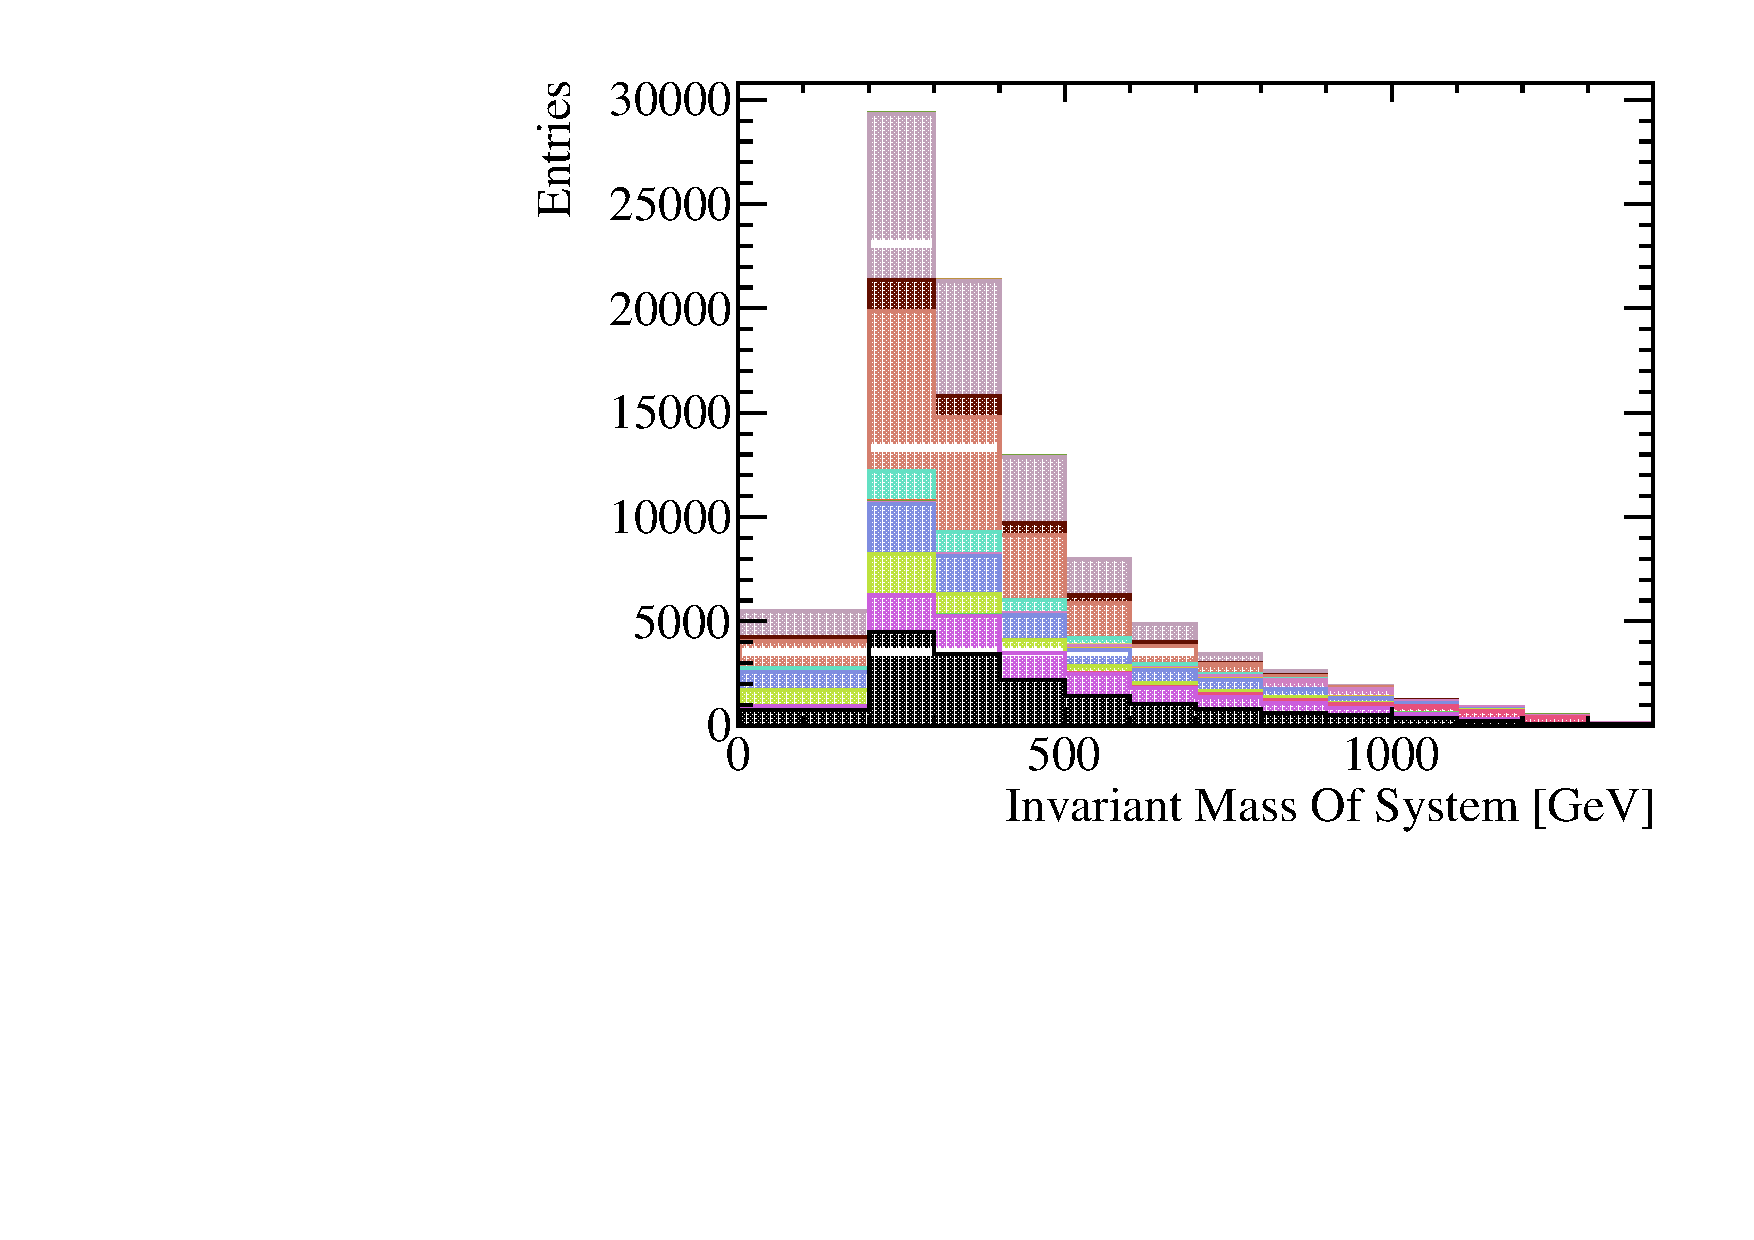
\includegraphics[width=0.5\textwidth]{PhysicsAnalysis/Plots/NuisanceFit/1400GeV/FitPlotMVV.pdf}}
\subfloat{\label{fig:signalbackgroundfitlegend}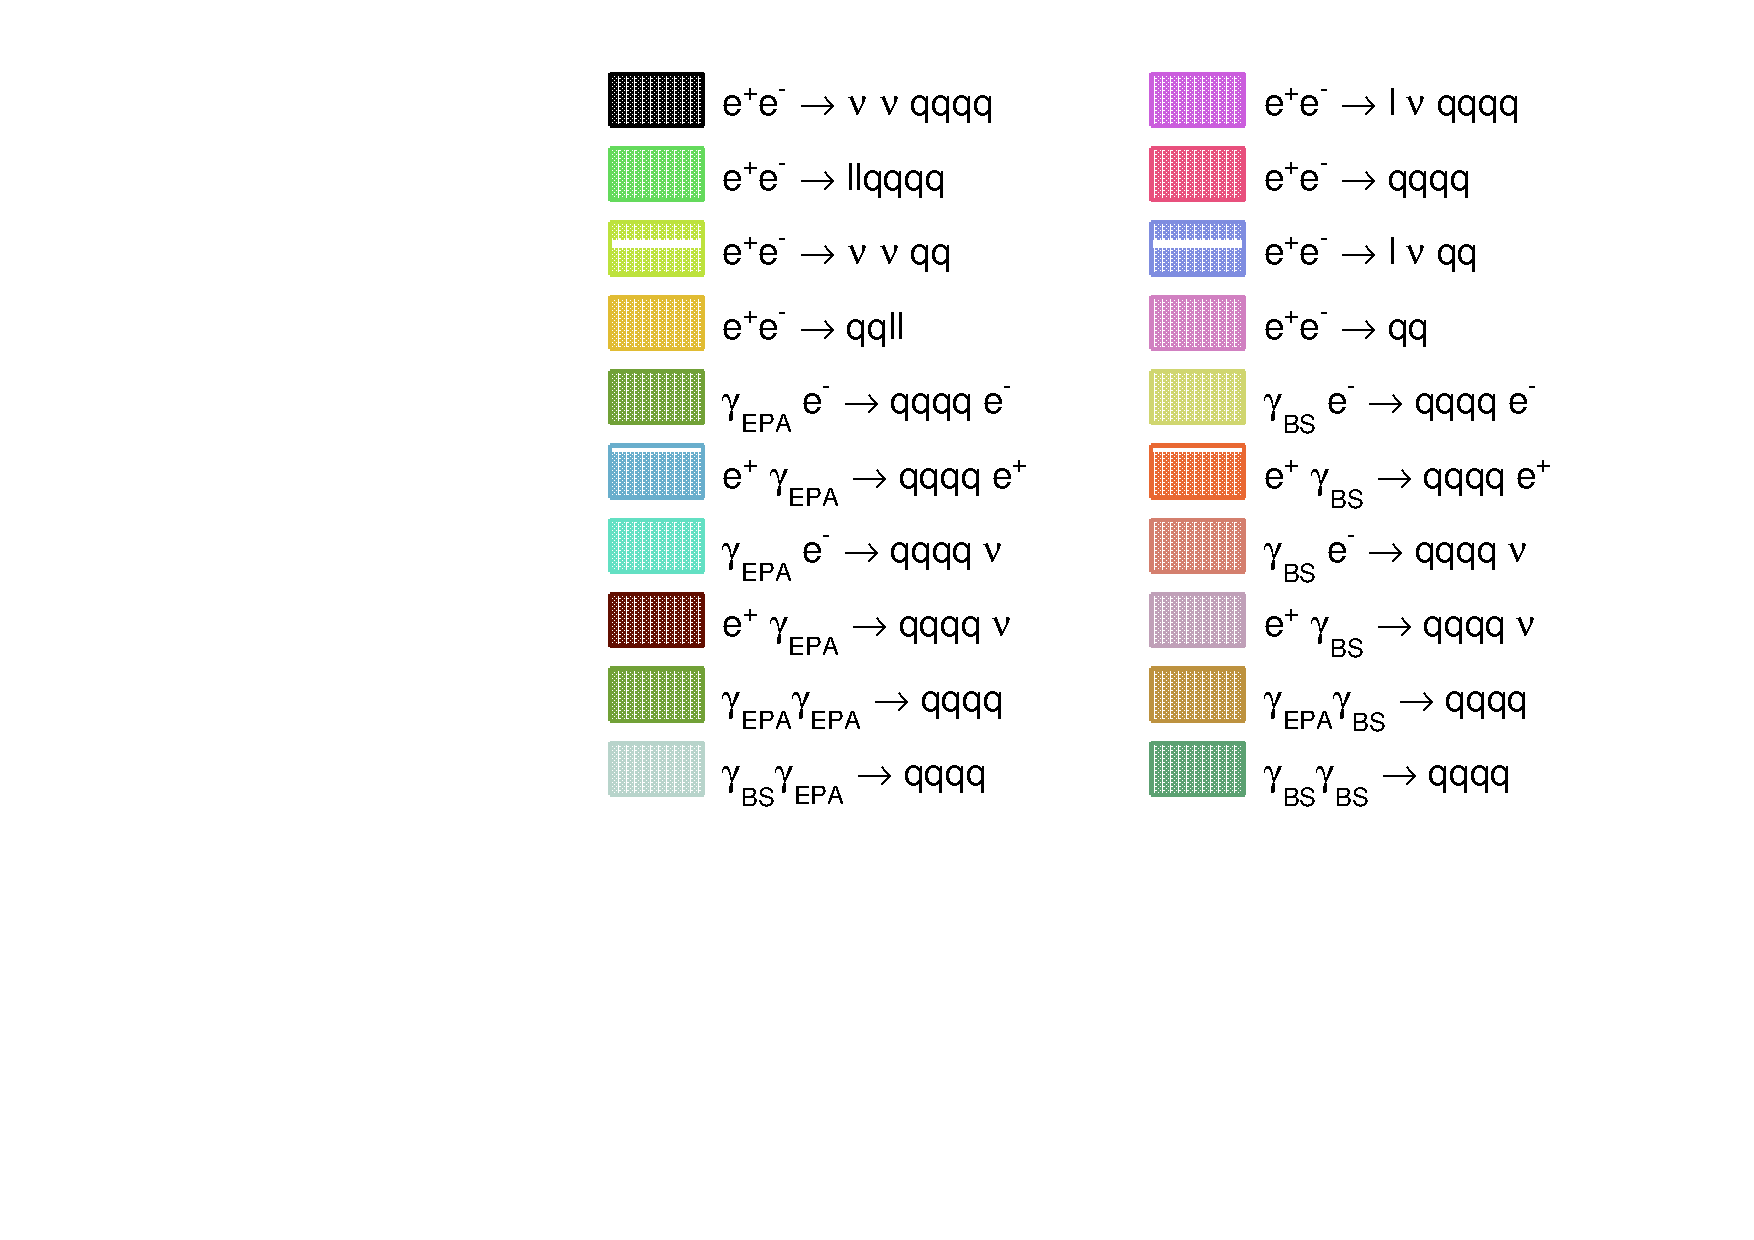
\includegraphics[width=0.5\textwidth]{PhysicsAnalysis/Plots/PreSelection/1400GeV/Legend.pdf}}
\caption[The distribution of the invariant mass of the system, $M_{VV}$, for both signal and background finals states that are used in the $\chi^{2}$ fit at $\sqrt{s}=1.4$~TeV.  The distribution includes effect of event selection and corresponds to an integrated luminosity of $\mathcal{L}_{int} = 1.5\text{ ab}^{-1}$.]{The distribution of the invariant mass of the system, $M_{VV}$, for both signal and background finals states that are used in the $\chi^{2}$ fit at $\sqrt{s}=1.4$~TeV.  The distribution includes effect of event selection and corresponds to an integrated luminosity of $\mathcal{L}_{int} = 1.5\text{ ab}^{-1}$.}
\label{fig:signalbackgroundfit}
\end{figure}

%========================================================================================

\subsection{Event Weight Interpolation Scheme}
\label{sec:eventweightsinterpolation}
In order to obtain a smooth $\chi^{2}$ surface a fine sampling of the event weights in the $\alpha_{4}$ and $\alpha_{5}$ space is required, however, it is unfeasible to generate a finely sampled grid of event weights on an event by event basis because event generation is highly CPU intensive.  To resolve this issue, an interpolation scheme was applied to determine the event weights within a sampled region of the $\alpha_{4}$ and $\alpha_{5}$ space.  This allows for an infinite sampling of the event weights in the space of $\alpha_{4}$ and $\alpha_{5}$ without having to call the generator an infinite number of times.

A bicubic interpolation scheme, cubic interpolation along the two dimensions, was applied to the event weights produced by the generator.  This procedure is best illustrated by figure \ref{fig:eventweights1400interpolated}, which shows the interpolated event weight surface superimposed with the raw event weights from the generator for four $\nu\nu\text{qqqq}$ events at $\sqrt{s}=1.4$~TeV.  This interpolation scheme produces a smooth and continuous surface that can be used for generating a smooth $\chi^{2}$ surface.  

\begin{figure}[h!]
\centering
\subfloat[]{\label{fig:weight1}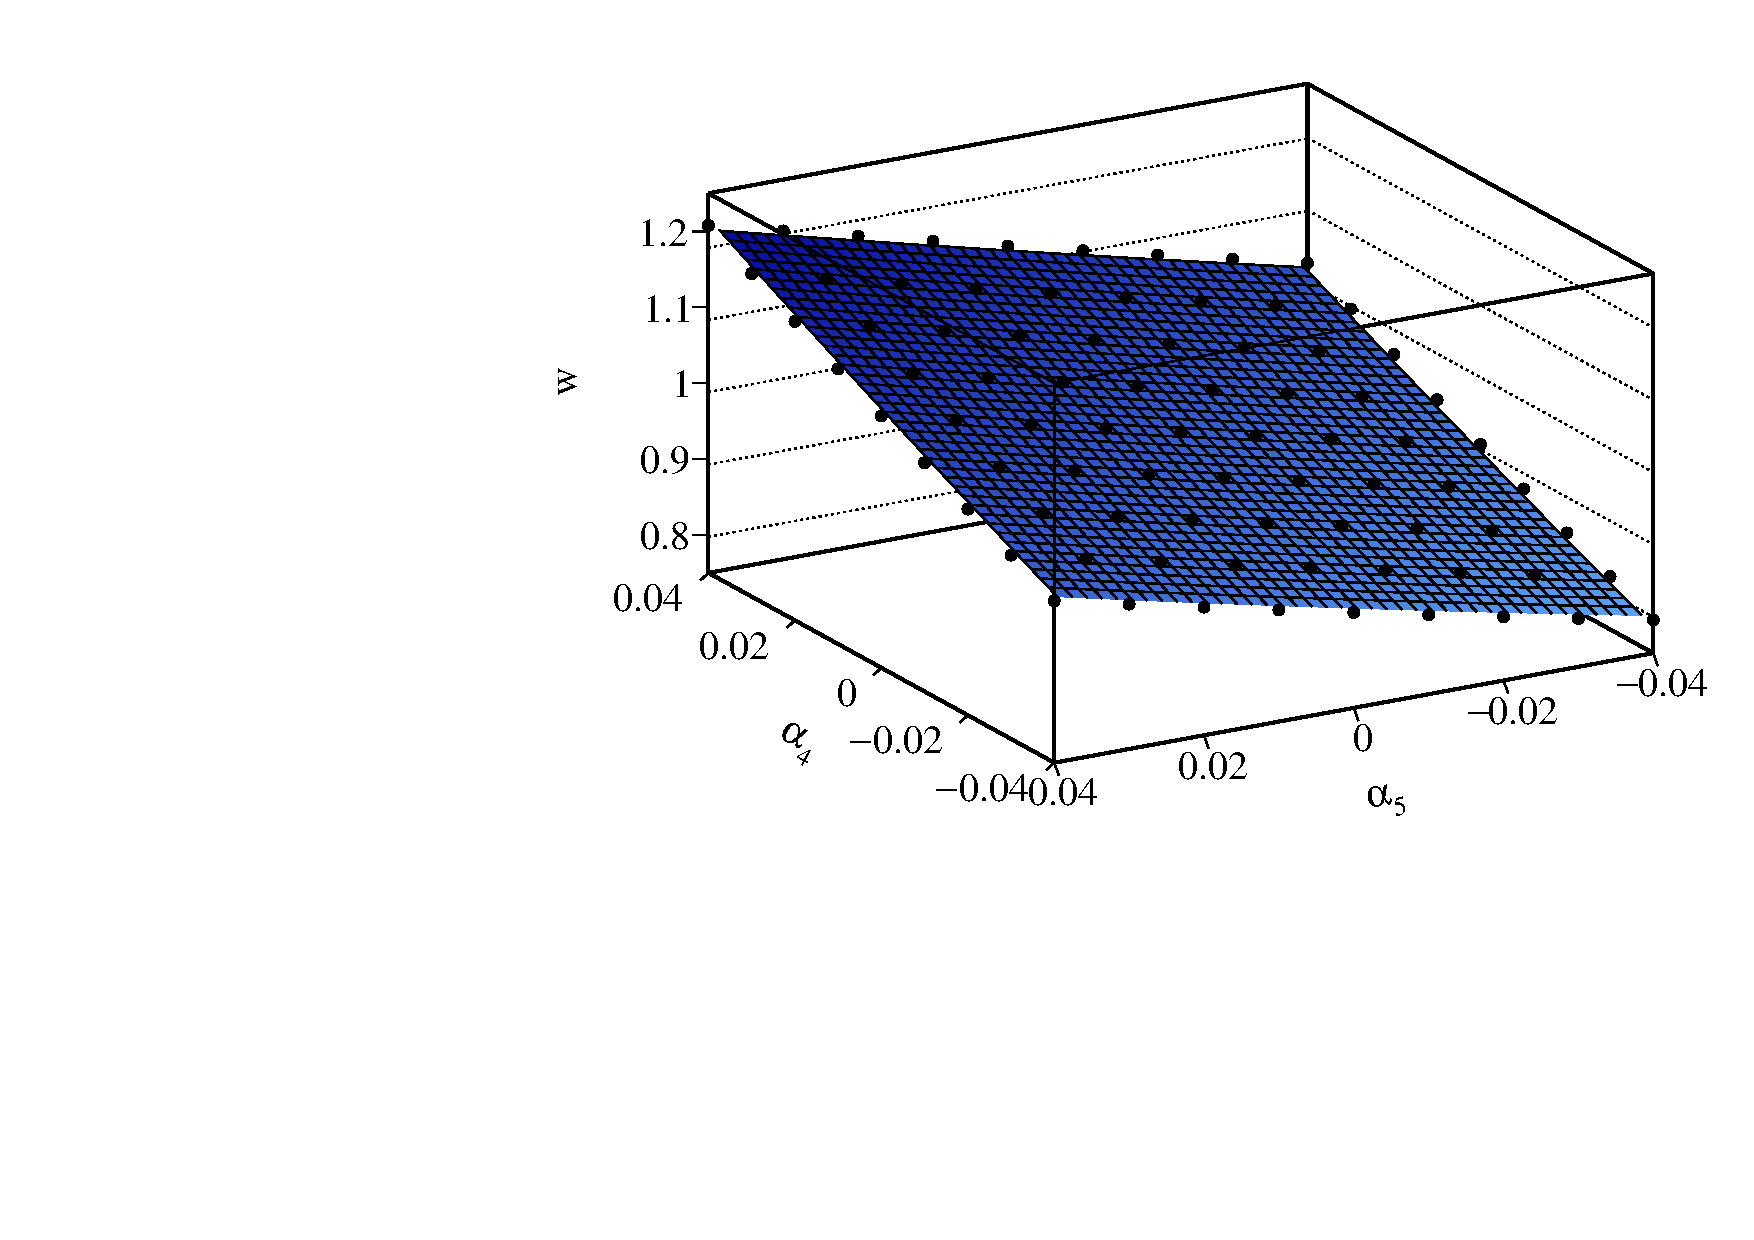
\includegraphics[width=0.5\textwidth]{PhysicsAnalysis/Plots/EventWeights/1400GeV/EventWeightsForEvent100001009_1400GeV_SPFOs_kt_0p70_10Bins_Start_0_End_10_1400GeV_Interpolated.pdf}}
\subfloat[]{\label{fig:weight2}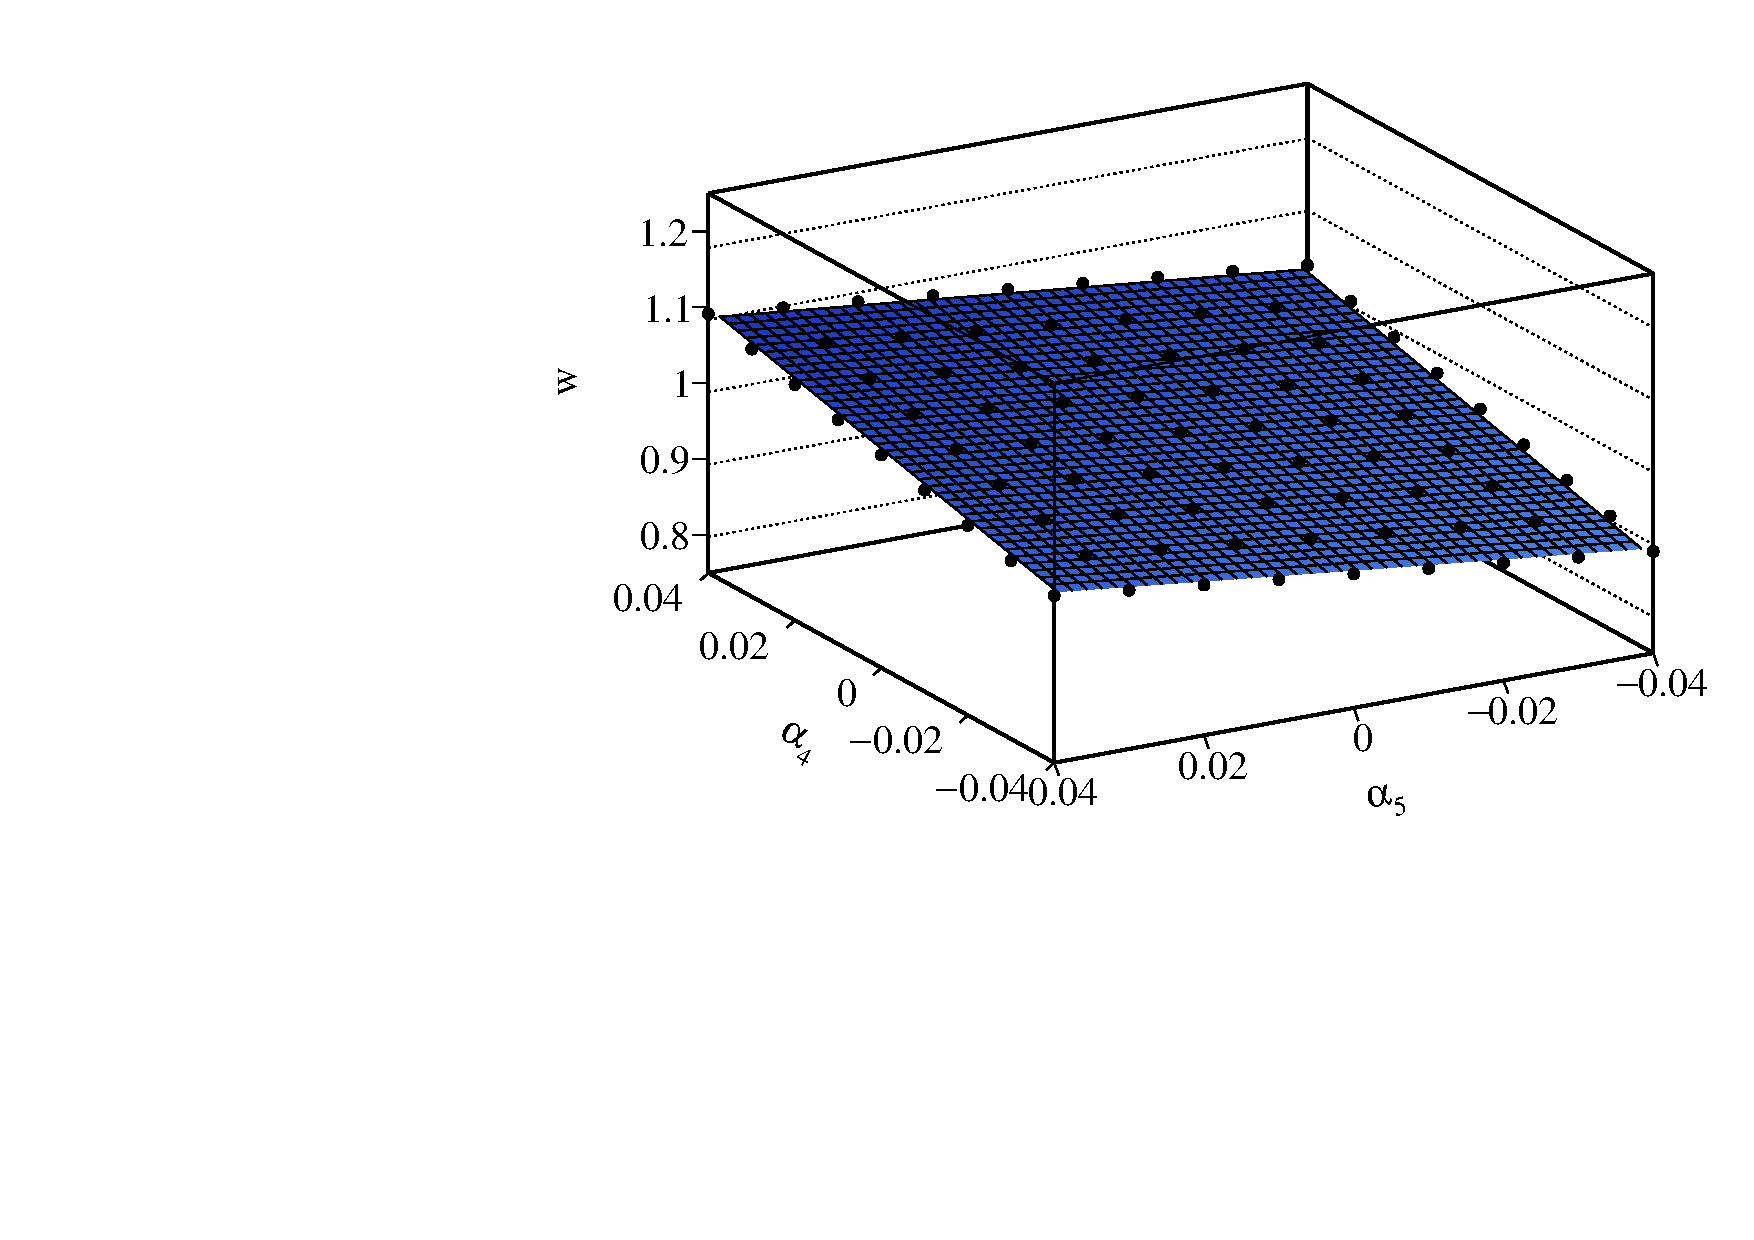
\includegraphics[width=0.5\textwidth]{PhysicsAnalysis/Plots/EventWeights/1400GeV/EventWeightsForEvent100001014_1400GeV_SPFOs_kt_0p70_10Bins_Start_0_End_10_1400GeV_Interpolated.pdf}} \hfill
\subfloat[]{\label{fig:weight3}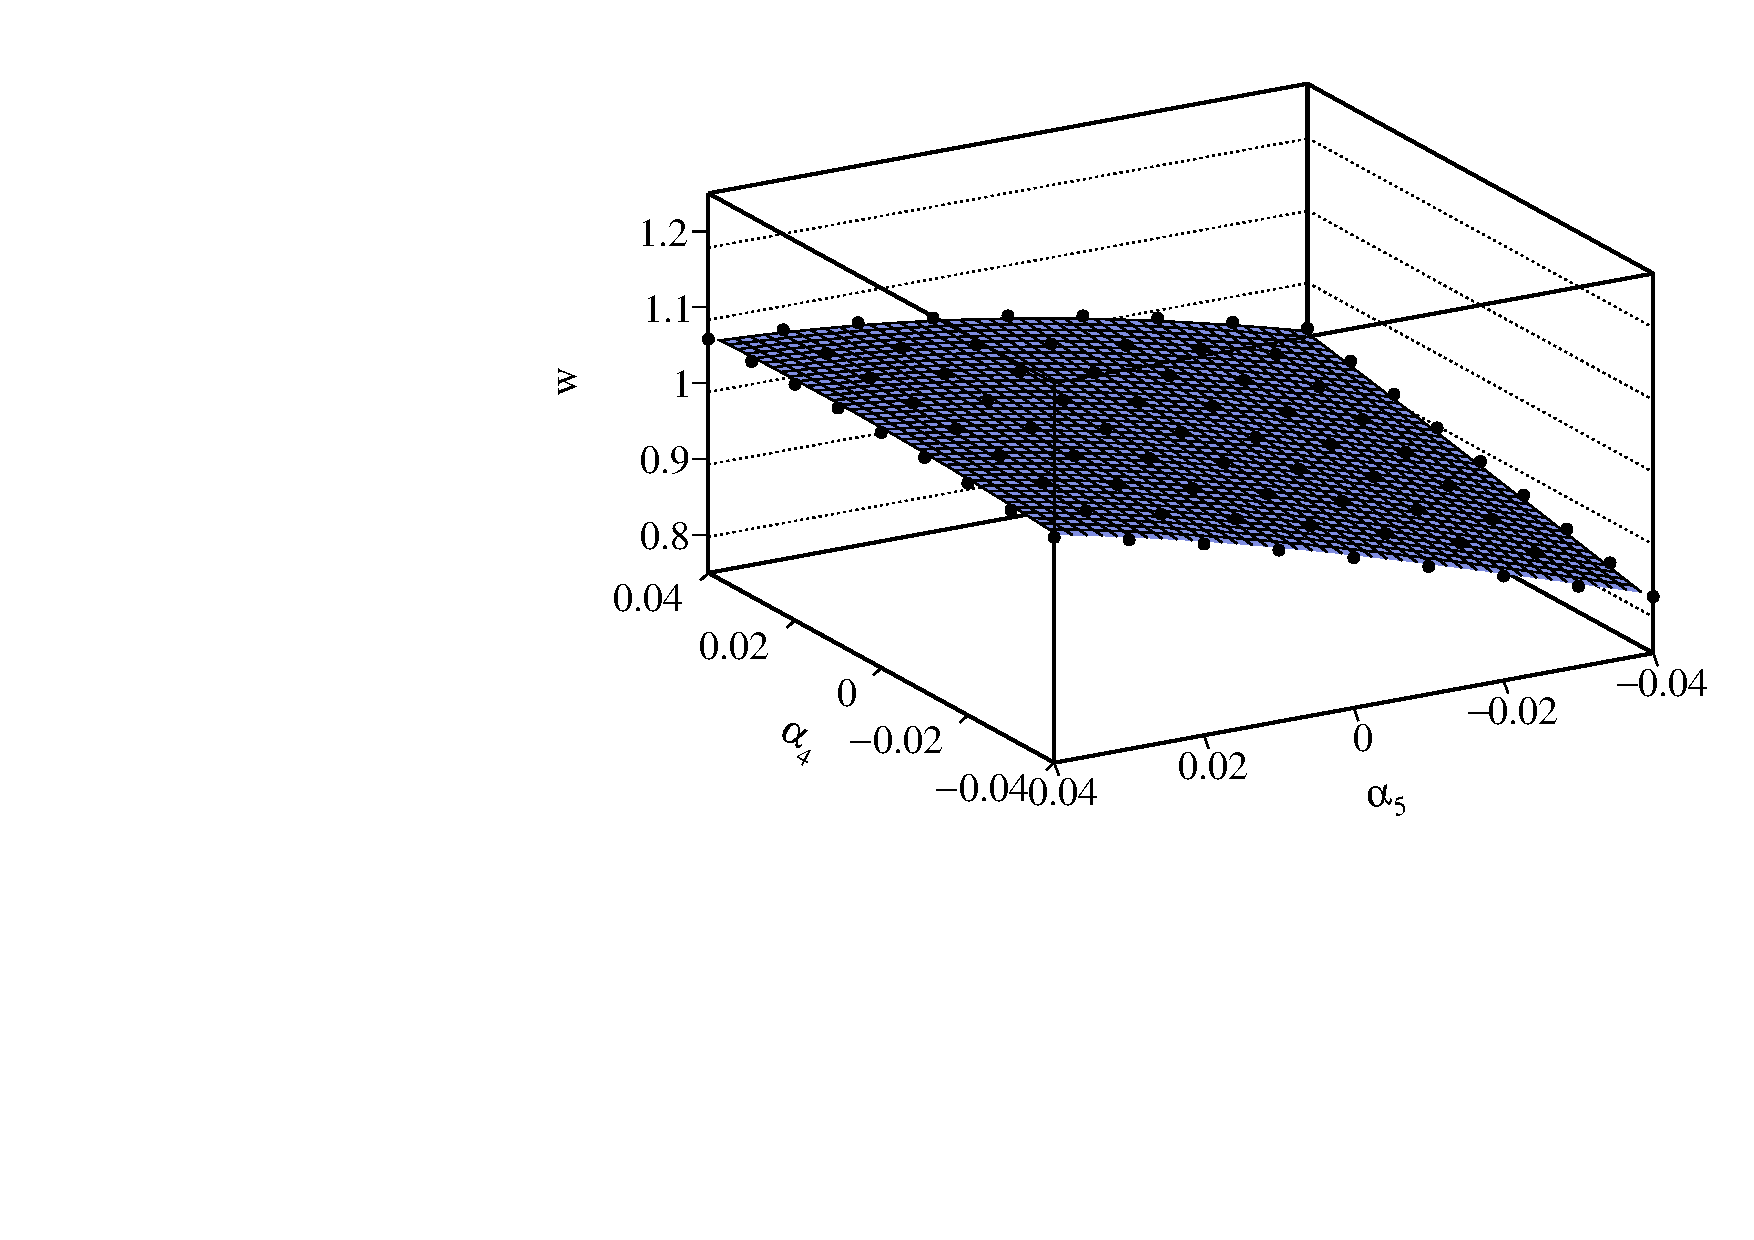
\includegraphics[width=0.5\textwidth]{PhysicsAnalysis/Plots/EventWeights/1400GeV/EventWeightsForEvent100001044_1400GeV_SPFOs_kt_0p70_10Bins_Start_0_End_10_1400GeV_Interpolated.pdf}}
\subfloat[]{\label{fig:weight4}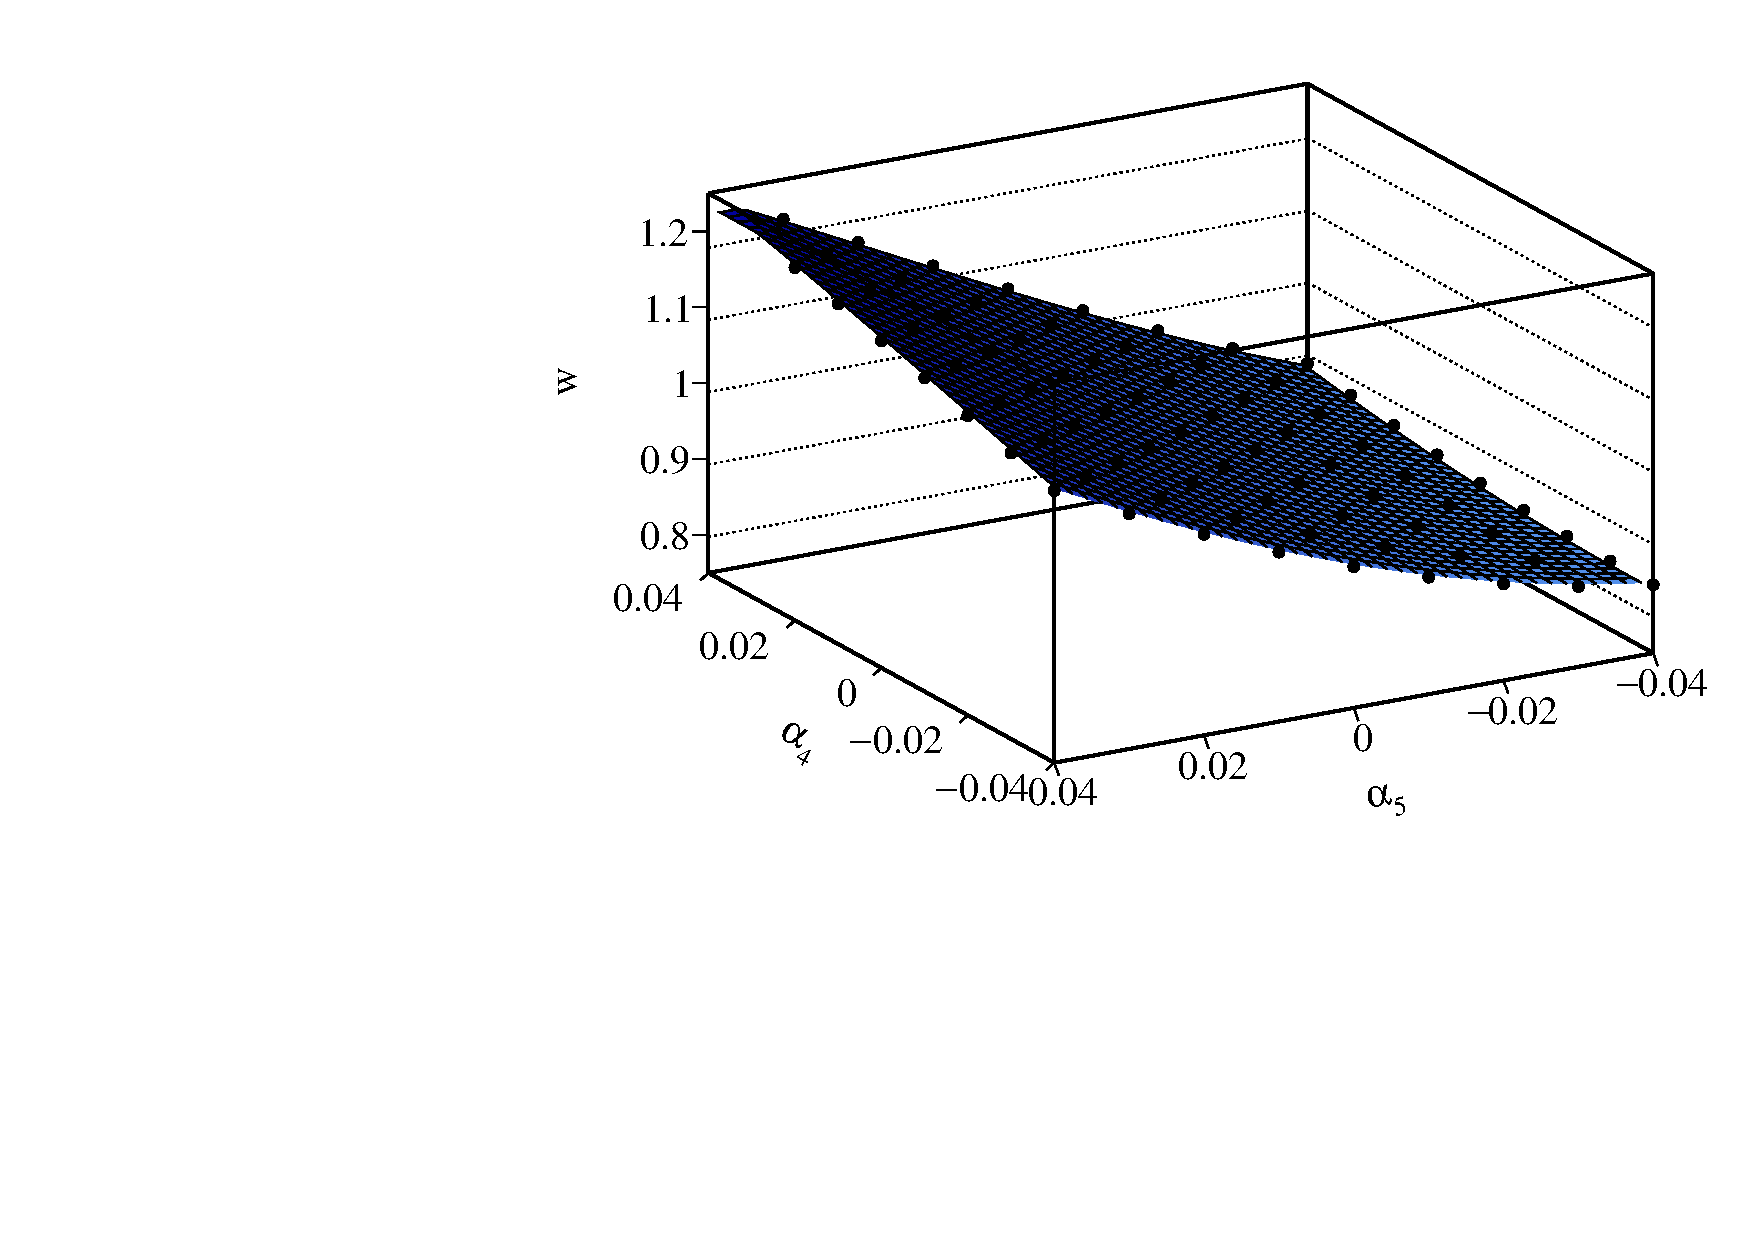
\includegraphics[width=0.5\textwidth]{PhysicsAnalysis/Plots/EventWeights/1400GeV/EventWeightsForEvent100001051_1400GeV_SPFOs_kt_0p70_10Bins_Start_0_End_10_1400GeV_Interpolated.pdf}}
\caption[The event weight, $w$, as a function of the anomalous couplings $\alpha_{4}$ and $\alpha_{5}$ for a selection of $\sqrt{s}=1.4$~TeV \nu{\nu}qqqq final state events.  The black circles show the event weight produced from the generator and the blue surface is determined using bicubic interpolation between these points.]{The event weight, $w$, as a function of the anomalous couplings $\alpha_{4}$ and $\alpha_{5}$ for a selection of $\sqrt{s}=1.4$~TeV \nu{\nu}qqqq final state events.  The black circles show the event weight produced from the generator and the blue surface is determined using bicubic interpolation between these points.}
\label{fig:eventweights1400interpolated}
\end{figure}

%========================================================================================
%========================================================================================

\section{Results}
The sensitivity of the CLIC experiment to the anomalous gauge couplings $\alpha_{4}$ and $\alpha_{5}$ at $\sqrt{s}=1.4$~TeV is shown in figure \ref{fig:finalresult1400GeV}.  This result shows the sensitivity after the application of preselection and MVA purposed to remove the included background channels.  These contours give a 68\% confidence limit for CLIC operating at $\sqrt{s}=1.4$~TeV of
%
\begin{equation}
-0.0082 < \alpha_{4} < 0.0116 \text{,} \\
-0.0055 < \alpha_{5} < 0.0078 \text{.}
\end{equation}

\begin{figure}[h!]
\centering
\subfloat[]{\label{fig:finalresult1400GeV}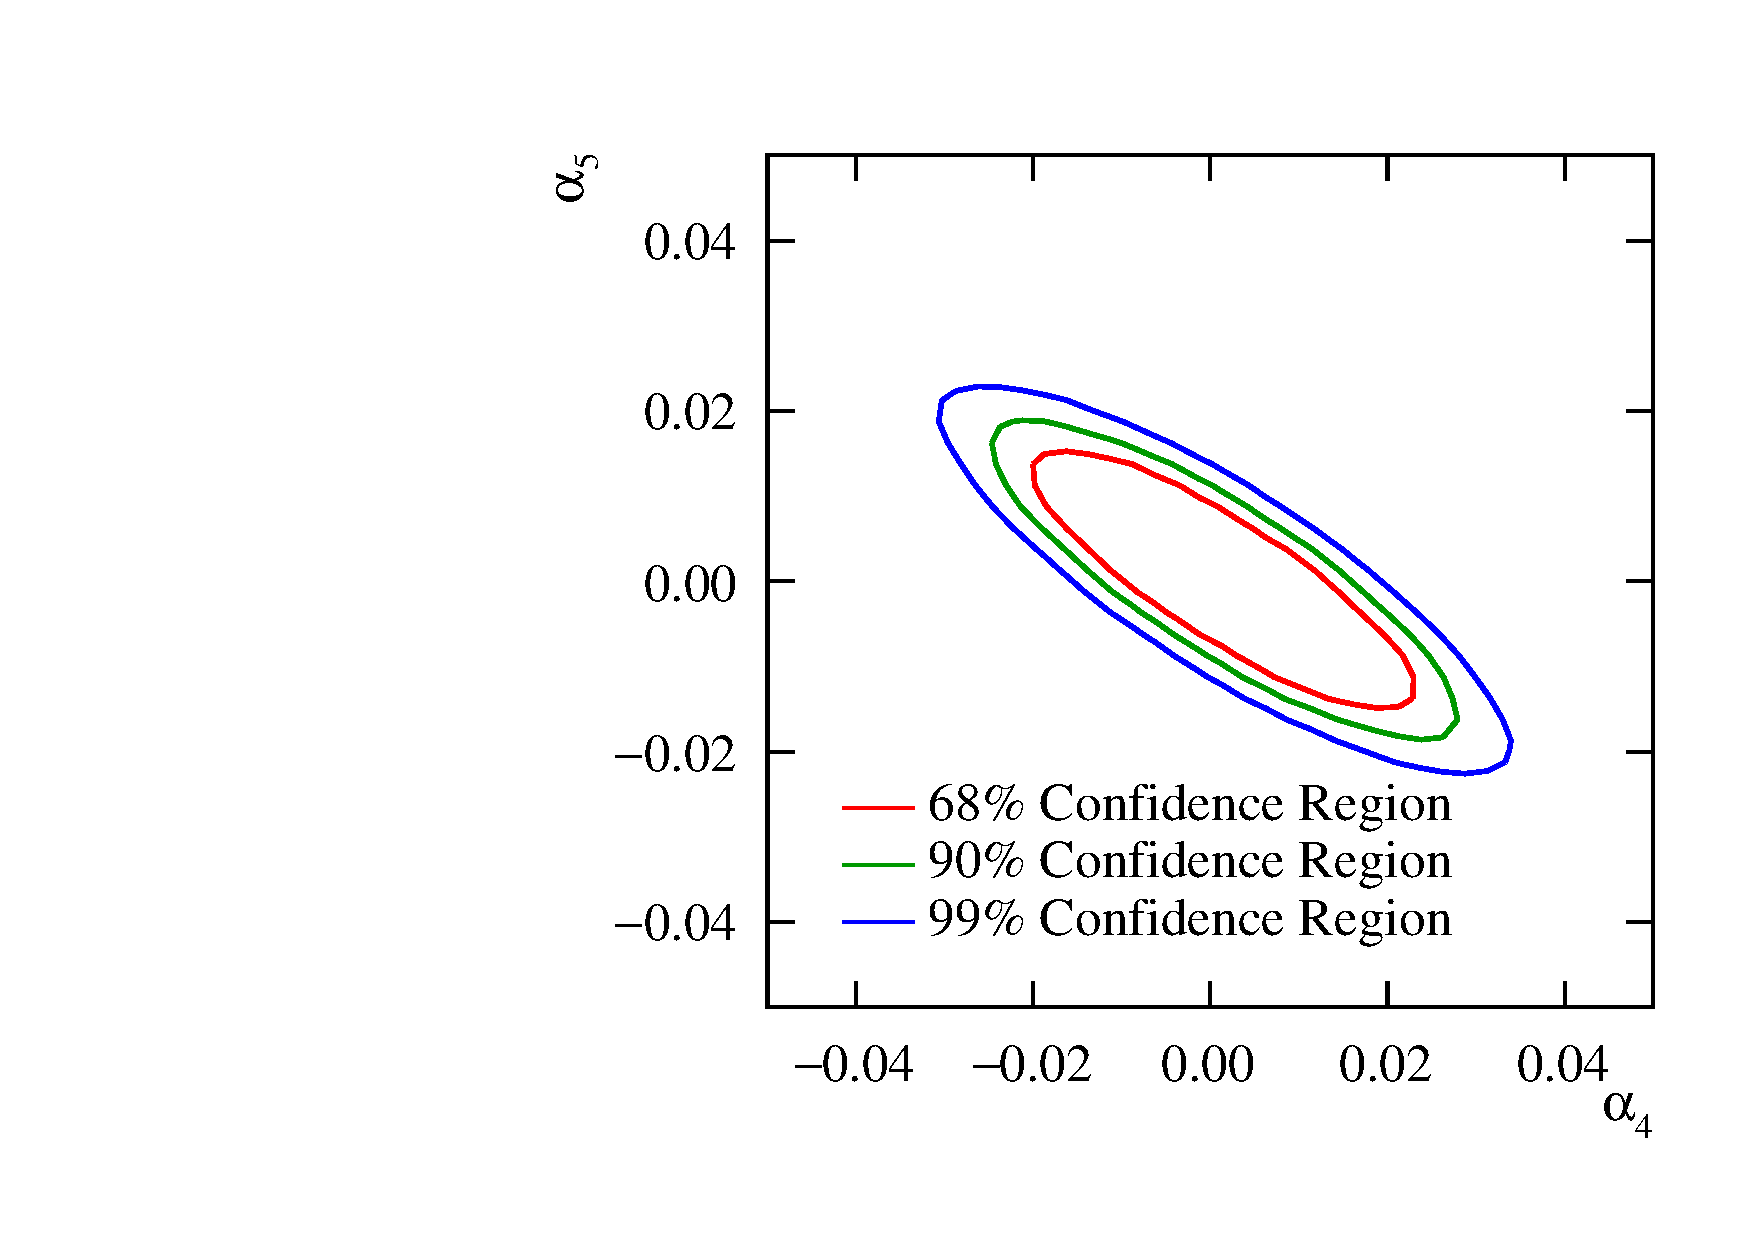
\includegraphics[width=0.5\textwidth]{PhysicsAnalysis/Plots/FinalResult/1400GeV/Final.pdf}}\hfill
\subfloat[]{\label{fig:a4finalresult1400GeV}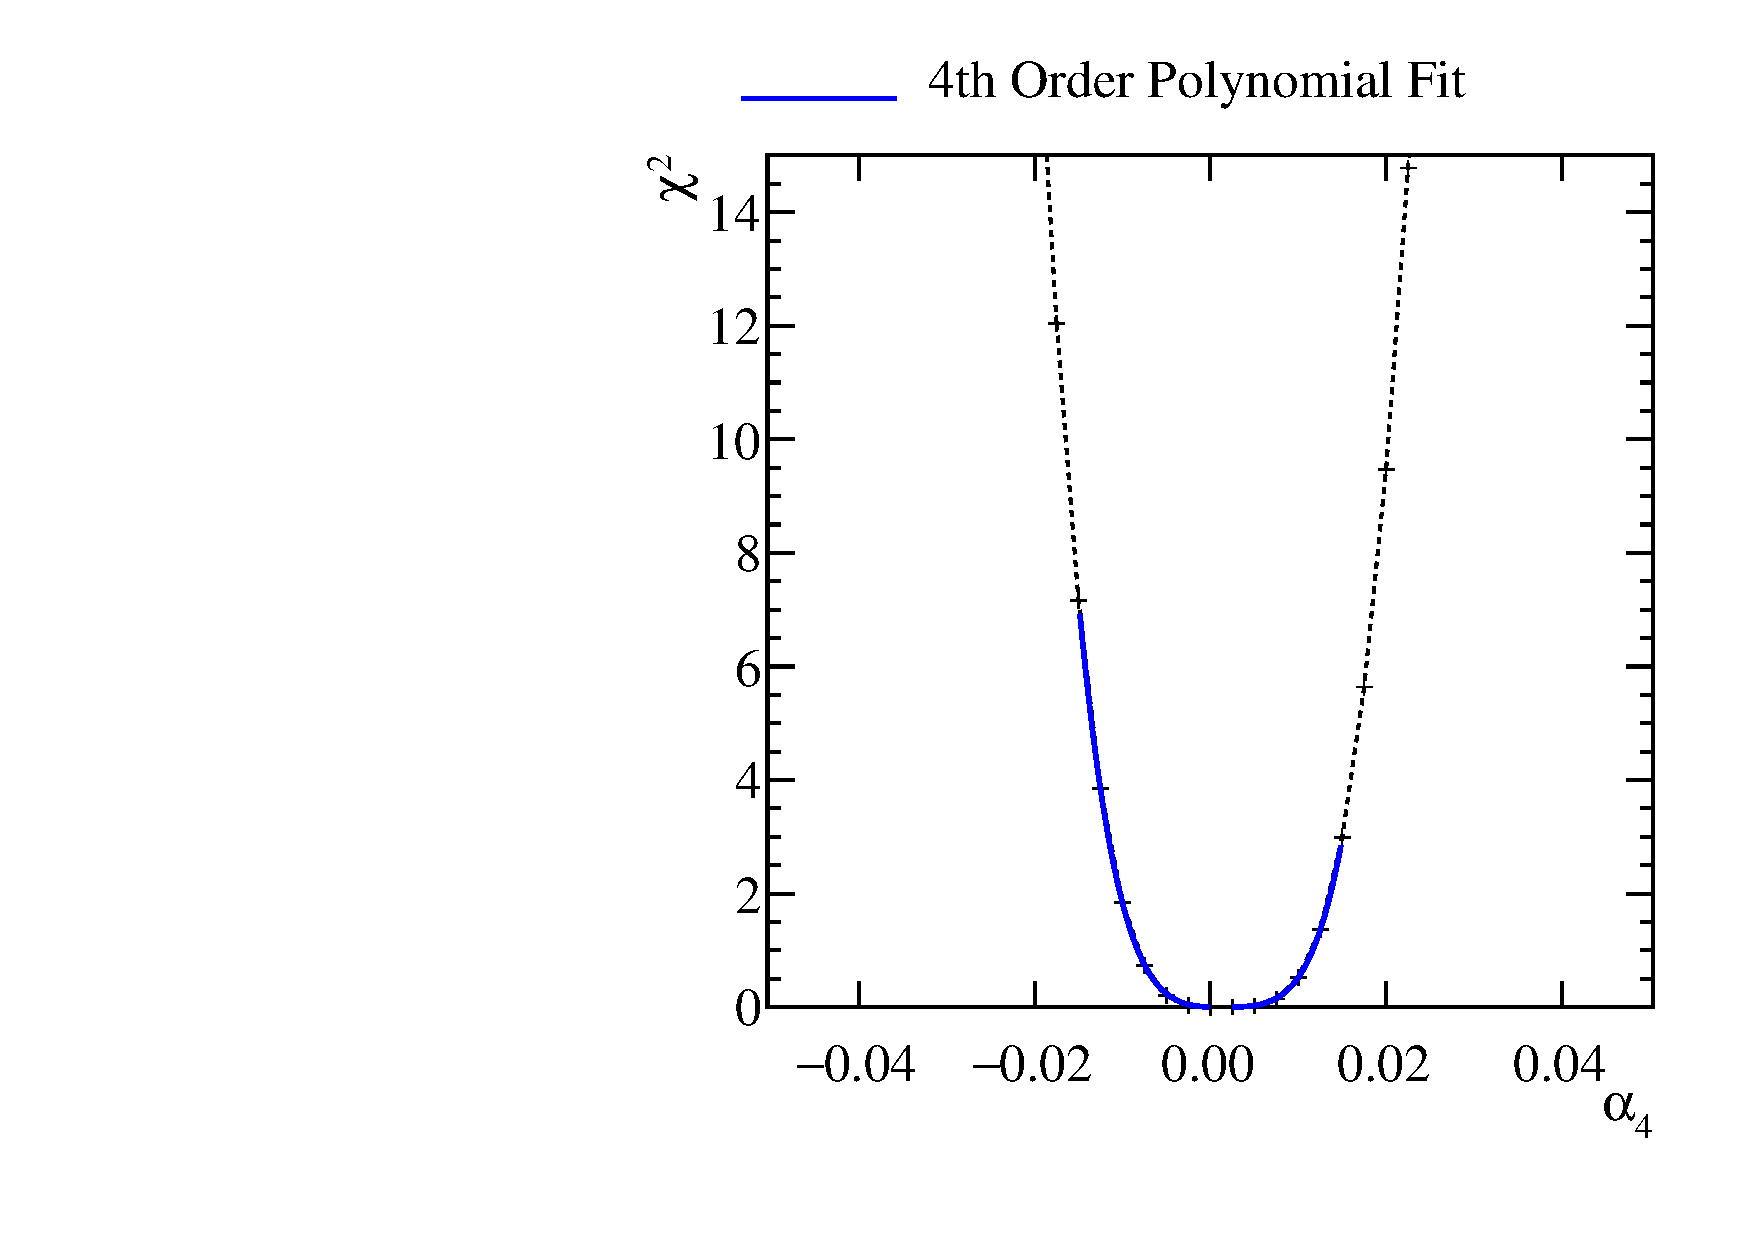
\includegraphics[width=0.5\textwidth]{PhysicsAnalysis/Plots/FinalResult/1400GeV/Final_alpha4.pdf}}
\subfloat[]{\label{fig:a5finalresult1400GeV}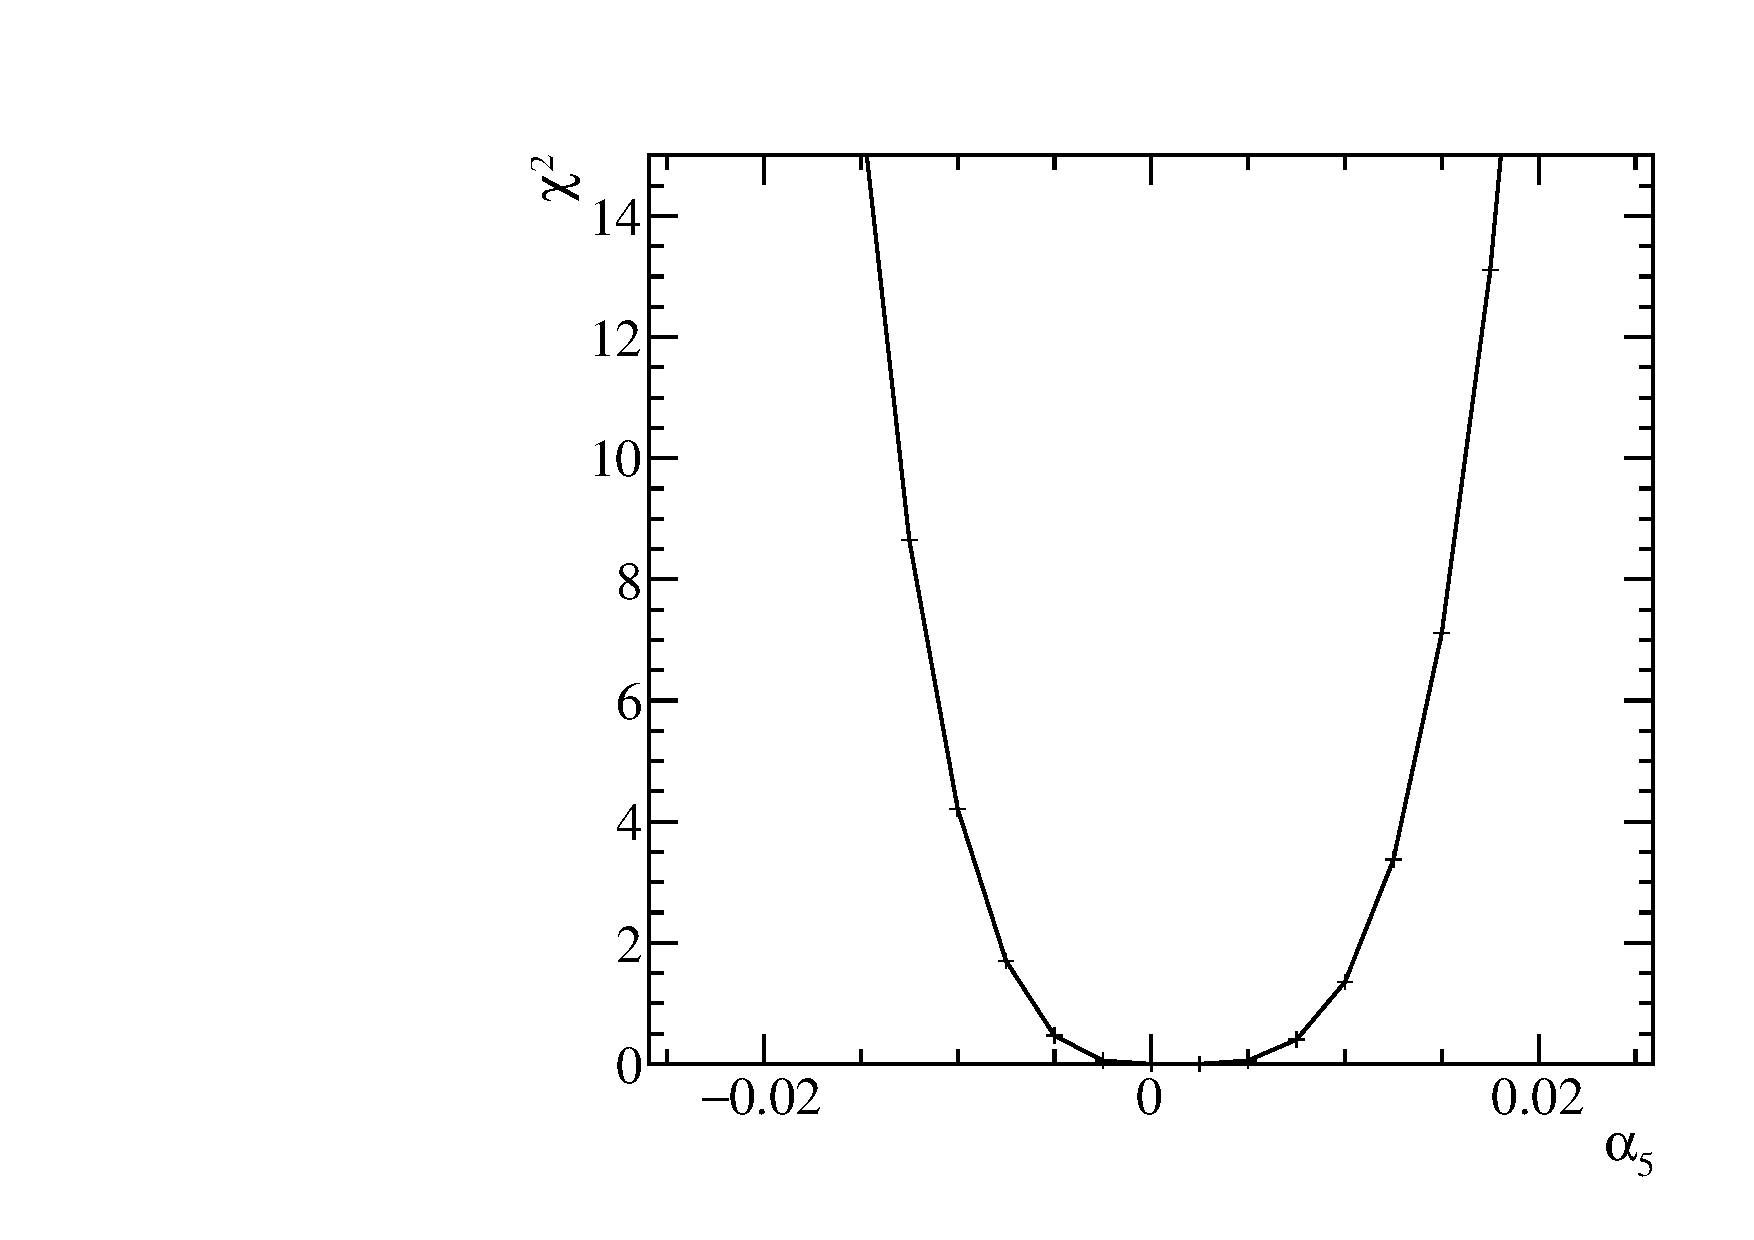
\includegraphics[width=0.5\textwidth]{PhysicsAnalysis/Plots/FinalResult/1400GeV/Final_alpha5.pdf}}
\caption[$\chi^{2}$ sensitivity distributions from a fit to $M_{VV}$ at $\sqrt{s}=1.4$~TeV.  Results include the effect of backgrounds after the application of a series of preselection cuts and MVA.  \protect\subref{fig:finalresult1400GeV} $\chi^{2}$ sensitivity contours in $\alpha_{4}$ and $\alpha_{5}$ space.  \protect\subref{fig:a4finalresult1400GeV} $\chi^{2}$ as a function of $\alpha_{4}$ assuming $\alpha_{5} = 0$.  \protect\subref{fig:a5finalresult1400GeV} $\chi^{2}$ as a function of $\alpha_{5}$ assuming $\alpha_{4} = 0$.]{$\chi^{2}$ sensitivity distributions from a fit to $M_{VV}$ at $\sqrt{s}=1.4$~TeV.  Results include the effect of backgrounds after the application of a series of preselection cuts and MVA.  \protect\subref{fig:finalresult1400GeV} $\chi^{2}$ sensitivity contours in $\alpha_{4}$ and $\alpha_{5}$ space.  \protect\subref{fig:a4finalresult1400GeV} $\chi^{2}$ as a function of $\alpha_{4}$ assuming $\alpha_{5} = 0$.  \protect\subref{fig:a5finalresult1400GeV} $\chi^{2}$ as a function of $\alpha_{5}$ assuming $\alpha_{4} = 0$.}
\label{fig:allfinalresult1400GeV}
\end{figure}

%========================================================================================

\subsection{Systematic Uncertainties}
\label{sec:systematics}
A source of systematic error in this experiment is the uncertainty on the cross-sections for the signal and background processes.  Based on the event selection summary shown in table \ref{table:selectionsummary1400GeV}, the dominant source of background in this analysis comes from the $\text{e}^{\pm}\gamma_{\text{BS}} \rightarrow \nu_{\text{e}}\text{qqqq}$ processes.  Therefore, uncertainties on the cross-section for these processes, as well as the signal process $\text{e}^{+}\text{e}^{-} \rightarrow \nu{\nu}\text{qqqq}$, will be considered.  

The uncertainty on the cross-section for a given process is included in the $\chi^{2}$ definition through the use of a nuisance parameter.  This procedure allows the cross-section for a process to fluctuate, however, the magnitude of the fluctuation, $r$, is moderated by an additional penalty term in the $\chi^{2}$ as follows
%
\begin{equation}
\chi^{2}(r) = \sum_{i} \frac{(O_{i} - E_{i}(r))^{2}}{E_{i}(r)} + \frac{(r-1)^{2}}{\sigma_{r}^{2}} \text{,}
\end{equation}
%
\noindent where $O_{i}$ is the observed, $\alpha_{4} = \alpha_{5} = 0$, bin content for bin $i$ in the distribution of $M_{VV}$ with no background fluctuations and $E_{i}(r)$ is the expected, $\alpha_{4} \neq 0$ and $\alpha_{5} \neq 0$, bin content for bin $i$ in the distribution of $M_{VV}$ where the cross-section for the process of interest has been scaled by a factor of $r$.  The sum $\sum_{i}$ runs over the bins in the $M_{VV}$ distribution.  The $\sigma_{r}$ variable is the width of the distribution of $r$, which indicates the uncertainty on the measurement of the cross-section of interest.  A $\chi^{2}$ surface is constructed in the space of $\alpha_{4}$ and $\alpha_{5}$ by minimising $\chi^{2}(r)$ at each point.  

The 68\% confidence region is shown with the inclusion of a nuisance parameter for the signal process $\text{e}^{+}\text{e}^{-} \rightarrow \nu{\nu}\text{qqqq}$ and the dominant background processes $\text{e}^{\pm}\gamma_{\text{BS}} \rightarrow \nu_{\text{e}}\text{qqqq}$ in figures \ref{fig:nuisance1400GeVsig} and \ref{fig:nuisance1400GeVbkg} respectively.  Minimal changes in sensitivity are observed when allowing the signal and dominant backgrounds to fluctuate.  This can be understood by considering the shape of the $M_{VV}$ distribution for the signal and dominant background processes, which is shown in figure \ref{fig:nuisanceexplanation1400GeV}.  These distribution shows that anomalous couplings primarily affect events with large invariant masses, while both the signal and dominant backgrounds peak at low invariant masses.  Therefore, by fluctuating the cross-section for the signal and dominant background processes, it is not possible to gain a significantly better match between the observed and expected bin contents in the $M_{VV}$ distribution.  This is encouraging as despite the $\text{e}^{\pm}\gamma_{\text{BS}} \rightarrow \nu_{\text{e}}\text{qqqq}$ backgrounds dominating the $\chi^{2}$ fit that determines the sensitivity of CLIC to the anomalous gauge couplings, precise knowledge of their cross-section is not crucial.  As the uncertainty on these cross-sections does not significantly effect the confidence regions, no cross-section uncertainties are accounted for when reporting the sensitivity of CLIC to the anomalous gauge couplings elsewhere in this analysis.   

\begin{figure}[h!]
\centering
\subfloat[]{\label{fig:nuisance1400GeVsig}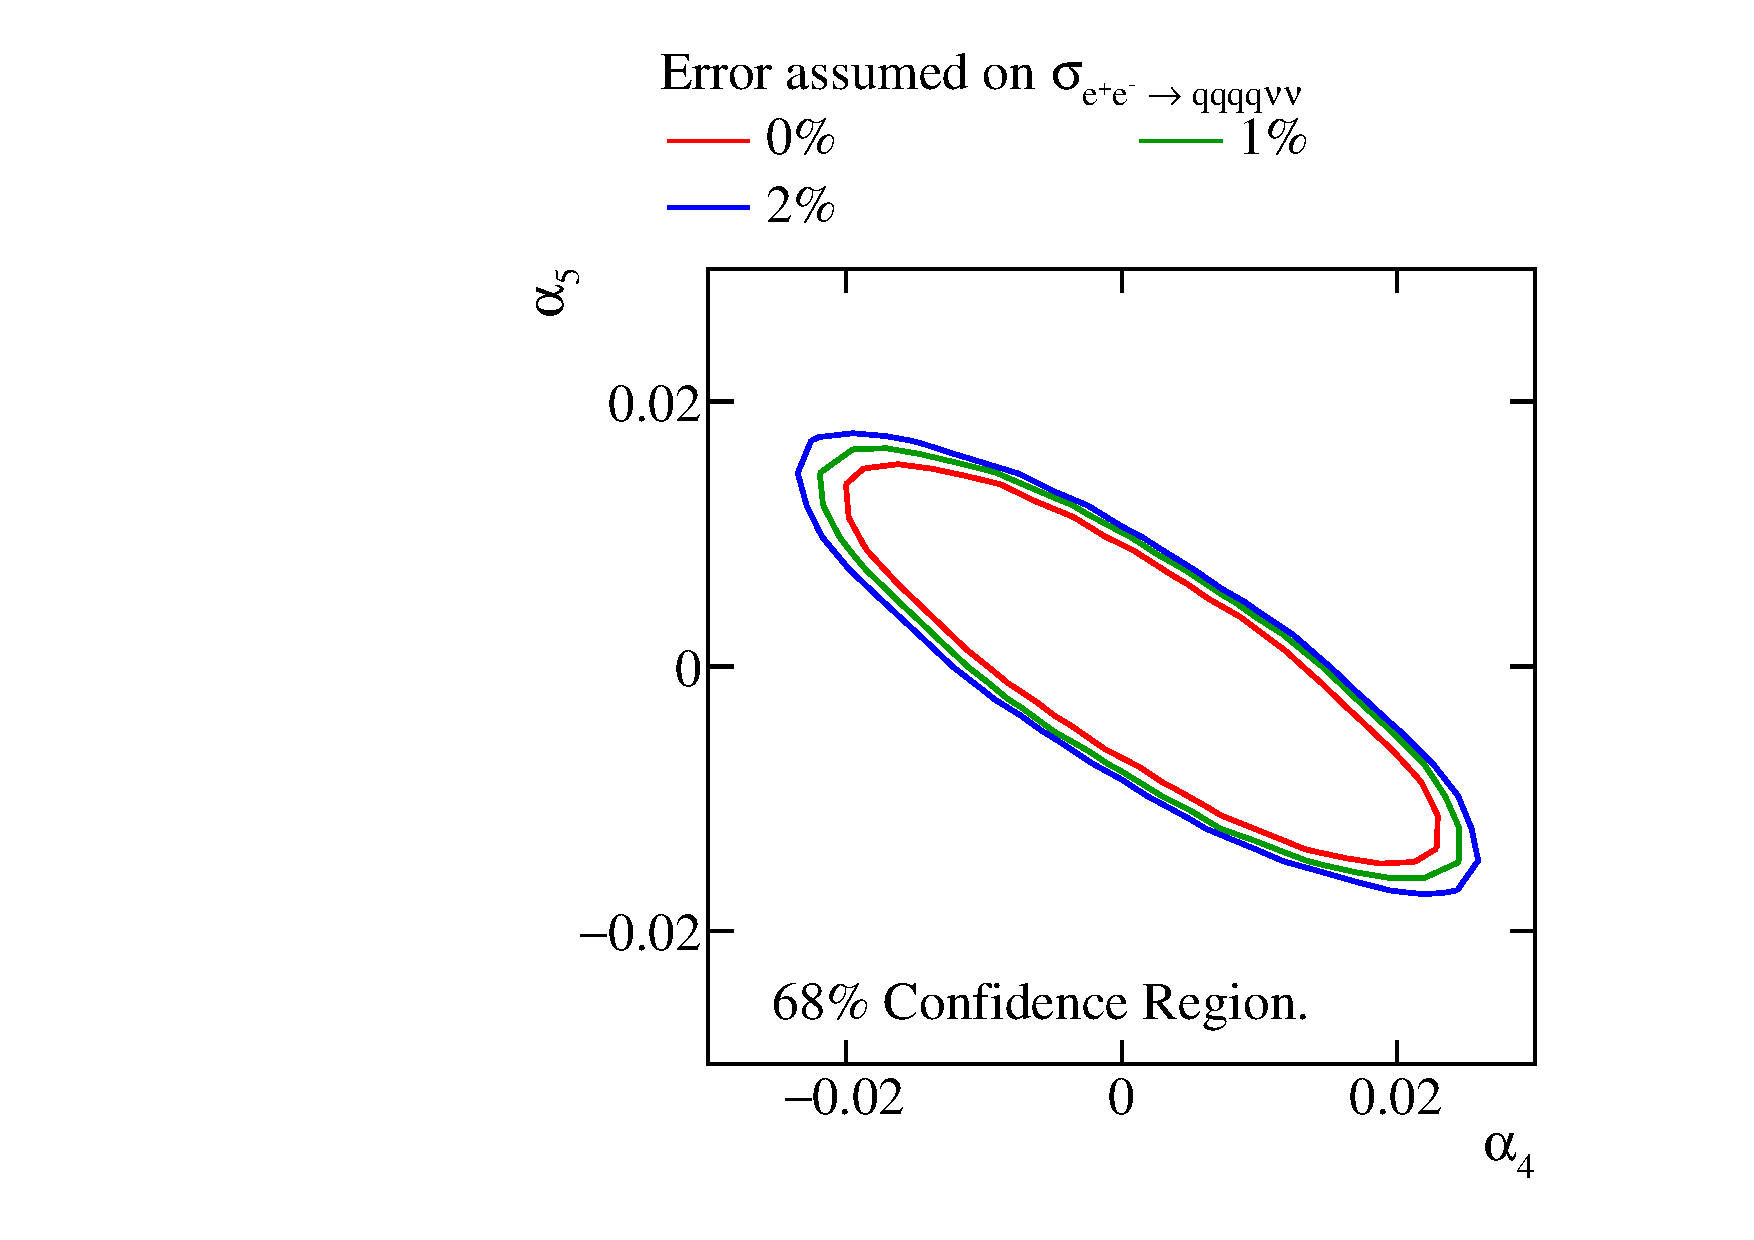
\includegraphics[width=0.5\textwidth]{PhysicsAnalysis/Plots/NuisanceFit/1400GeV/NuisanceSignal.pdf}}\hfill
\subfloat[]{\label{fig:nuisance1400GeVbkg}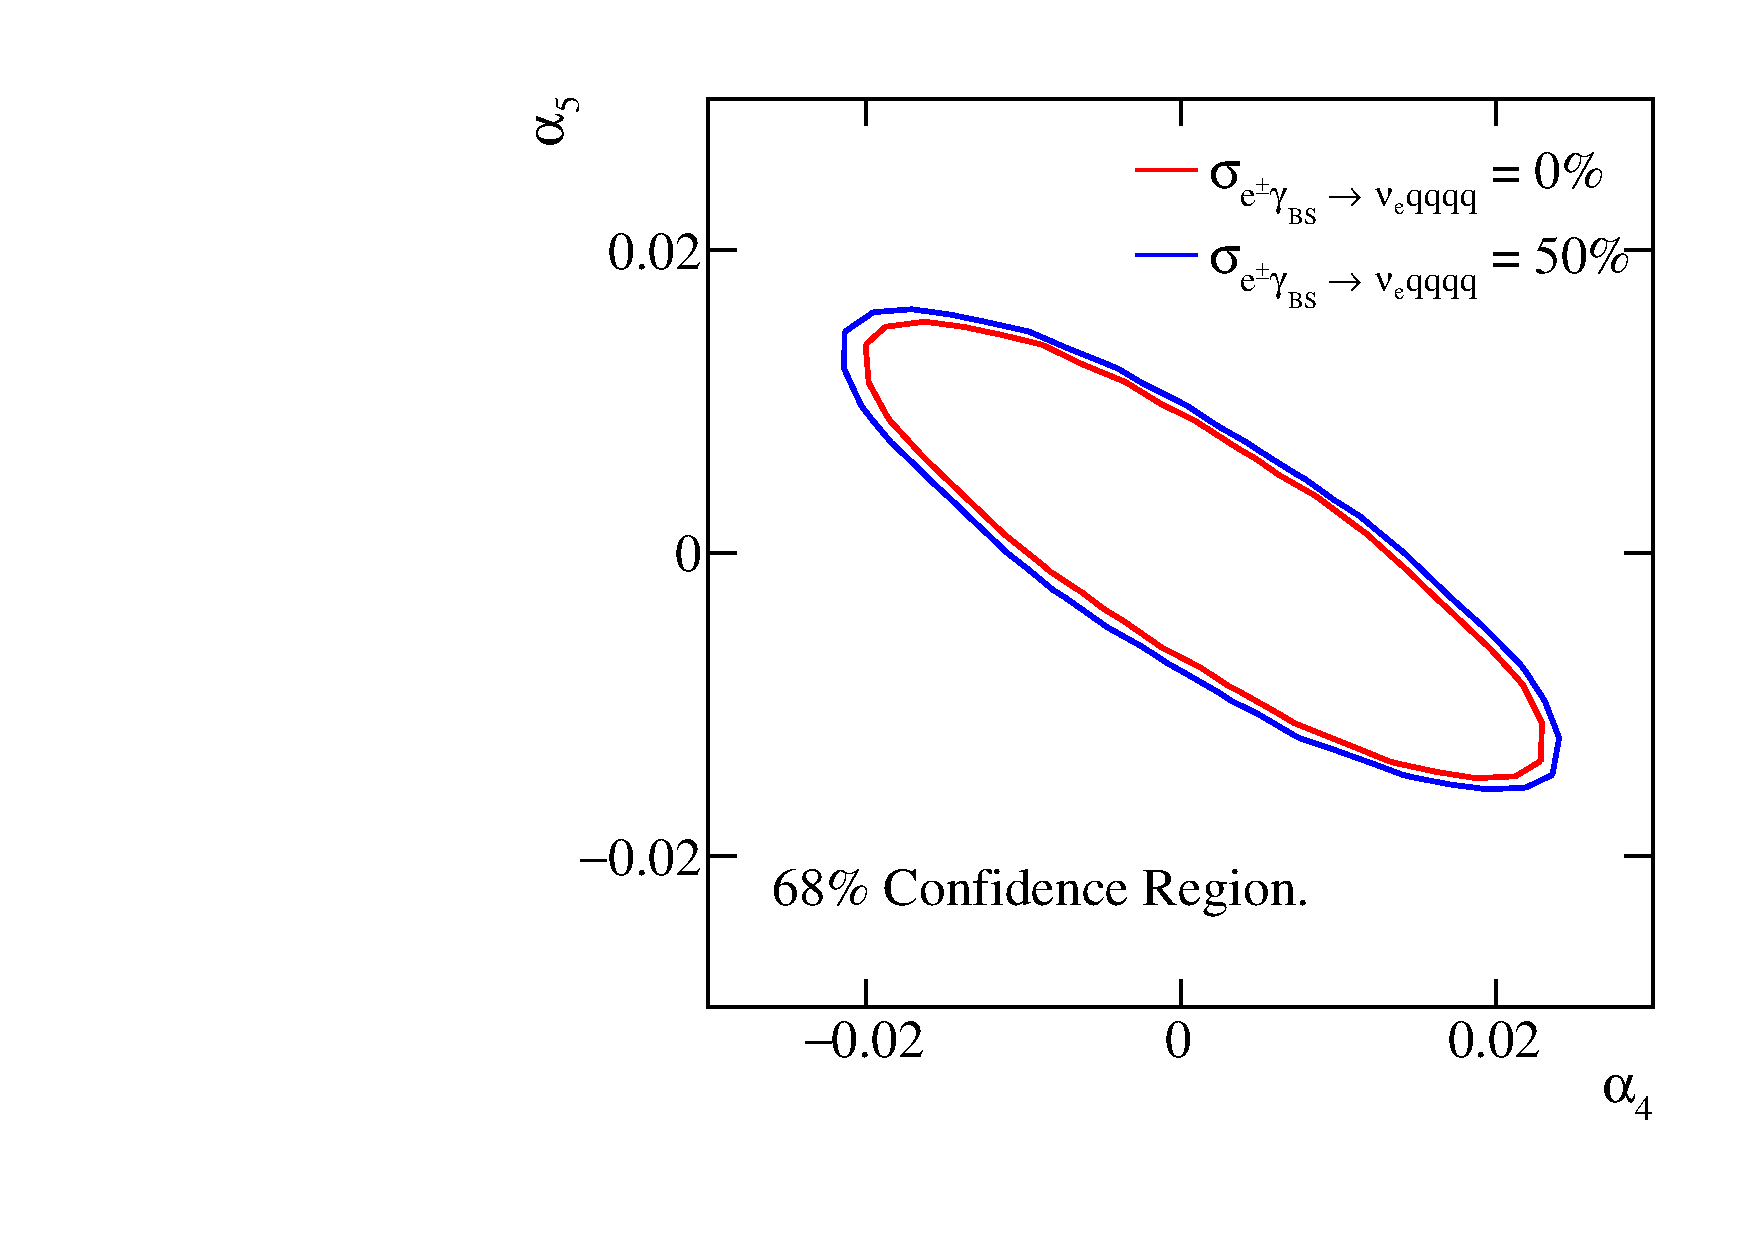
\includegraphics[width=0.5\textwidth]{PhysicsAnalysis/Plots/NuisanceFit/1400GeV/Nuisance.pdf}}
\caption[The 68\% confidence region including the effect of uncertainties in the cross-section for \protect\subref{fig:nuisance1400GeVsig} the signal process $\text{e}^{+}\text{e}^{-} \rightarrow \nu{\nu}\text{qqqq}$ and \protect\subref{fig:nuisance1400GeVbkg} the dominant background processes $\text{e}^{\pm}\gamma_{\text{BS}} \rightarrow \nu_{\text{e}}\text{qqqq}$.]{The 68\% confidence region including the effect of uncertainties in the cross-section for \protect\subref{fig:nuisance1400GeVsig} the signal process $\text{e}^{+}\text{e}^{-} \rightarrow \nu{\nu}\text{qqqq}$ and \protect\subref{fig:nuisance1400GeVbkg} the dominant background processes $\text{e}^{\pm}\gamma_{\text{BS}} \rightarrow \nu_{\text{e}}\text{qqqq}$.}
\label{fig:nuisance1400GeV}
\end{figure}

\begin{figure}[h!]
\centering
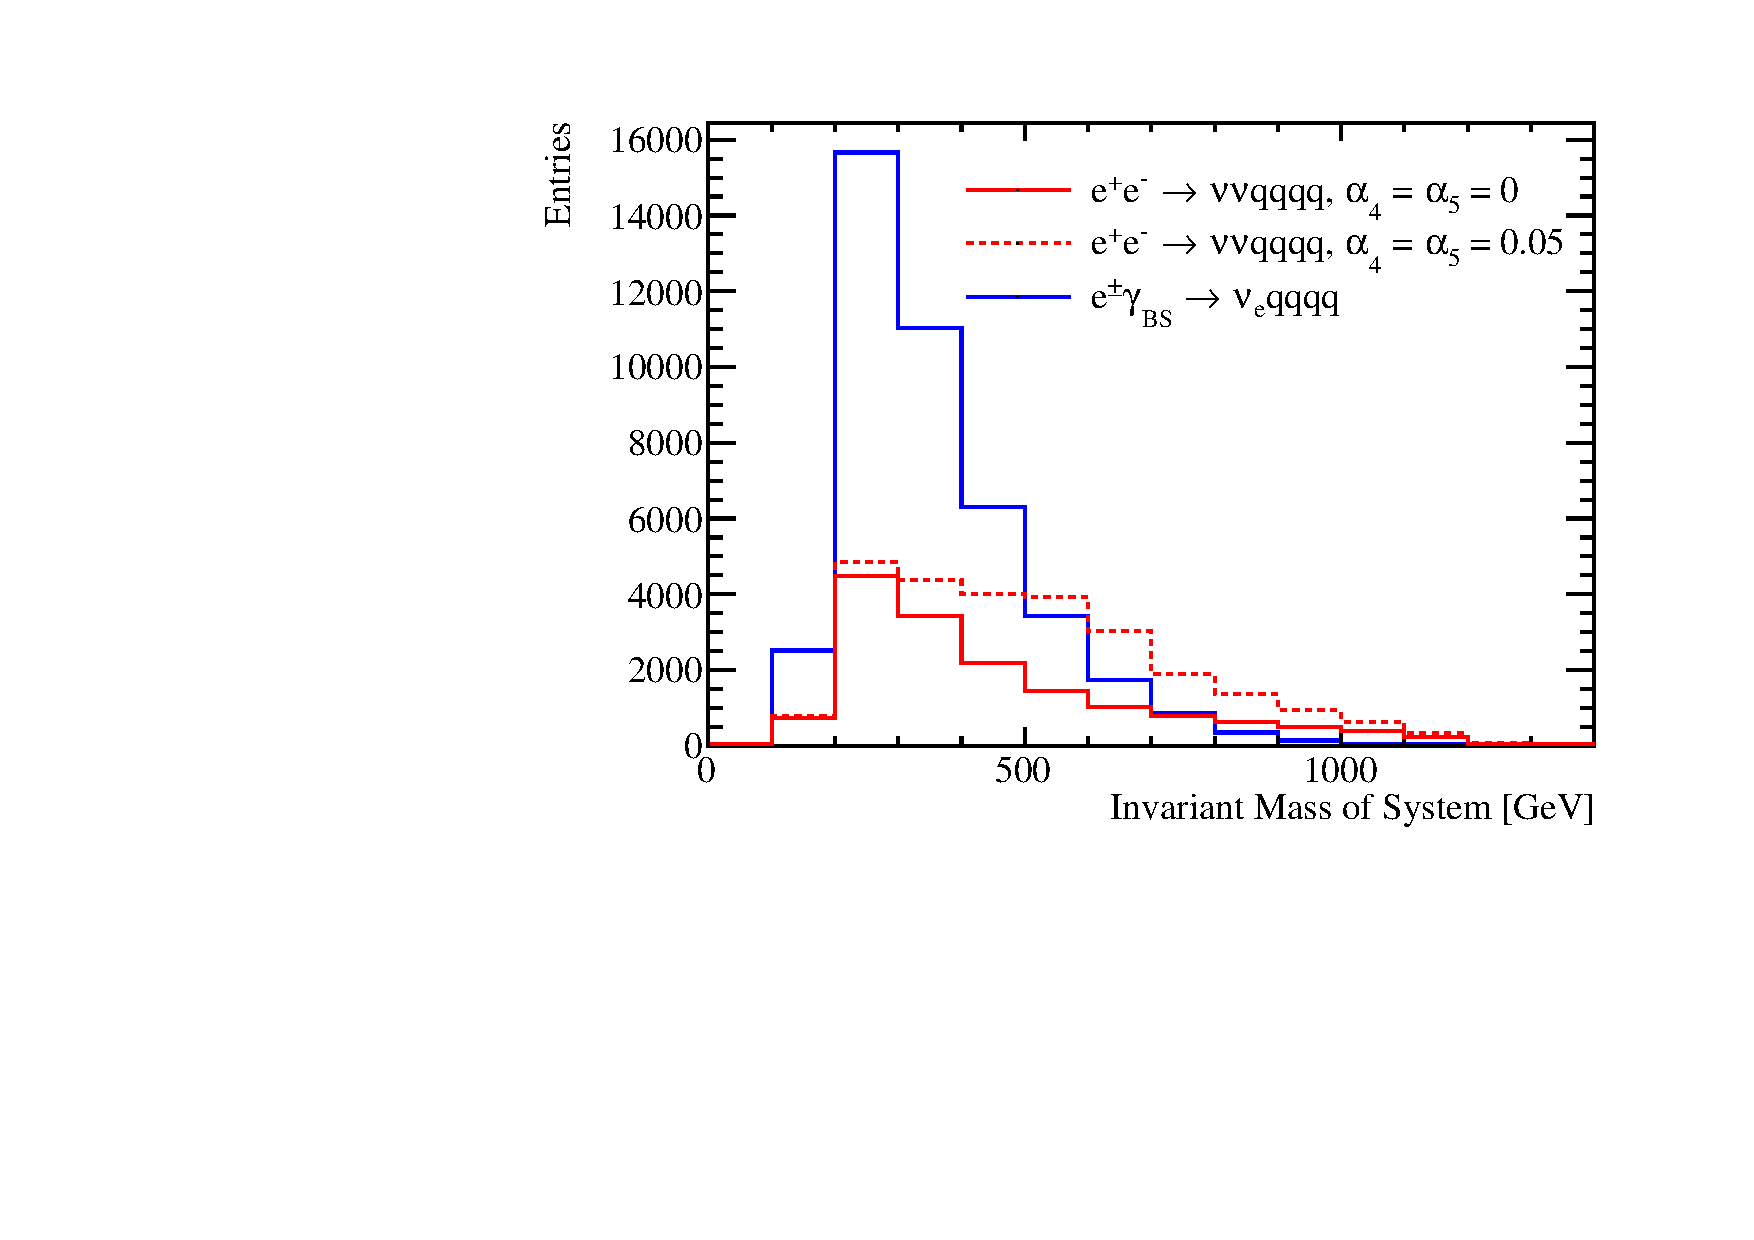
\includegraphics[width=0.75\textwidth]{PhysicsAnalysis/Plots/NuisanceFit/1400GeV/NuisanceExplanation.pdf}
\caption[Distributions of $M_{VV}$ for the $\text{e}^{+}\text{e}^{-} \rightarrow \nu{\nu}\text{qqqq}$ signal process, with and without the effect from anomalous couplings, and the combined dominant background processes $\text{e}^{\pm}\gamma_{\text{BS}} \rightarrow \nu_{\text{e}}\text{qqqq}$.  All distributions include the effect of event selection and correspond to an integrated luminosity of $\mathcal{L}_{int} = 1.5\text{ ab}^{-1}$.]{Distributions of $M_{VV}$ for the $\text{e}^{+}\text{e}^{-} \rightarrow \nu{\nu}\text{qqqq}$ signal process, with and without the effect from anomalous couplings, and the combined dominant background processes $\text{e}^{\pm}\gamma_{\text{BS}} \rightarrow \nu_{\text{e}}\text{qqqq}$.  All distributions include the effect of event selection and correspond to an integrated luminosity of $\mathcal{L}_{int} = 1.5\text{ ab}^{-1}$.}
\label{fig:nuisanceexplanation1400GeV}
\end{figure}

%========================================================================================
%========================================================================================

\section{Sensitivity at $\sqrt{s}=3$~TeV}
The anomalous gauge coupling sensitivity study described in this chapter was repeated for CLIC operating at $\sqrt{s}=3$~TeV.  As this analysis largely mirrors that of the $\sqrt{s}=1.4$~TeV analysis, this section focuses on the differences between the two analyses.  

The signal and background final states for the $\sqrt{s}=3$~TeV analysis were identical to those used for the $\sqrt{s}=1.4$~TeV analysis.  Cross-sections for these processes at $\sqrt{s}=3$~TeV are given in table \ref{table:crosssection3000GeV}.  The data analysis and event selection procedures used for the $\sqrt{s}=3$~TeV analysis mirrored those used for the $\sqrt{s}=1.4$~TeV analysis.  

\begin{table}[h!]
\centering
\begin{tabular}{ l r r }
\hline
Final State & Cross-Section [fb]  \\ 
\hline
$\text{e}^{+}\text{e}^{-} \rightarrow \nu{\nu}\text{qqqq}$ & 71.5 \\
$\text{e}^{+}\text{e}^{-} \rightarrow \nu\text{lqqqq}$ & 106.6 \\
$\text{e}^{+}\text{e}^{-} \rightarrow \text{llqqqq}$ & 169.3 \\
$\text{e}^{+}\text{e}^{-} \rightarrow \text{qqqq}$ & 546.5 \\
$\text{e}^{+}\text{e}^{-} \rightarrow \nu{\nu}\text{qq}$ & 1317.5 \\
$\text{e}^{+}\text{e}^{-} \rightarrow \nu\text{lqq}$ & 5560.9 \\
$\text{e}^{+}\text{e}^{-} \rightarrow \text{llqq}$ & 3319.6 \\
$\text{e}^{+}\text{e}^{-} \rightarrow \text{qq}$ & 2948.9 \\
$\text{e}^{-}\gamma_{\text{EPA}} \rightarrow \text{e}^{-}\text{qqqq}$ & 287.8 \\
$\text{e}^{-}\gamma_{\text{BS}} \rightarrow \text{e}^{-}\text{qqqq}$ & 1268.6 \\
$\text{e}^{+}\gamma_{\text{EPA}} \rightarrow \text{e}^{+}\text{qqqq}$ & 287.8 \\
$\text{e}^{+}\gamma_{\text{BS}} \rightarrow \text{e}^{+}\text{qqqq}$ & 1267.3 \\
$\text{e}^{-}\gamma_{\text{EPA}} \rightarrow \nu_{\text{e}}\text{qqqq}$ & 54.2 \\
$\text{e}^{-}\gamma_{\text{BS}} \rightarrow \nu_{\text{e}}\text{qqqq}$ & 262.5 \\
$\text{e}^{+}\gamma_{\text{EPA}} \rightarrow \overline{\nu}_{\text{e}}\text{qqqq}$ & 54.2 \\
$\text{e}^{+}\gamma_{\text{BS}} \rightarrow \overline{\nu}_{\text{e}}\text{qqqq}$ & 262.3 \\
$\gamma_{\text{EPA}}\gamma_{\text{EPA}} \rightarrow \text{qqqq}$ & 402.7 \\
$\gamma_{\text{EPA}}\gamma_{\text{BS}} \rightarrow \text{qqqq}$ & 2423.1 \\
$\gamma_{\text{BS}}\gamma_{\text{EPA}} \rightarrow \text{qqqq}$ & 2420.6 \\
$\gamma_{\text{BS}}\gamma_{\text{BS}} \rightarrow \text{qqqq}$ & 13050.3 \\
\hline
\end{tabular}
\caption[Cross-sections of signal and background processes at $\sqrt{s}=3$~TeV]{Cross-sections of signal and background processes at $\sqrt{s}=3$~TeV.  In the above table q represents u, $\bar{\text{u}}$, d, $\bar{\text{d}}$, s, $\bar{\text{s}}$, c, $\bar{\text{c}}$, b or $\bar{\text{b}}$;  l represents $\text{e}^{\pm}$, $\mu^{\pm}$ or $\tau^{\pm}$; and $\nu$ represents $\nu_{\text{e}}$, $\overline{\nu}_{\text{e}}$, $\nu_{\mu}$, $\overline{\nu}_{\mu}$, $\nu_{\tau}$ and $\overline{\nu}_{\tau}$.  The EPA and BS subscript on the incoming photon indicates whether the photon is generated from the equivalent photon approximation or beamstrahlung.}
\label{table:crosssection3000GeV}
\end{table}

Jet finding was performed using the longitudinally invariant $k_{t}$ algorithm as described in section \ref{sec:jetpairing}.  The jet algorithm configuration was optimised using the sensitivity of CLIC to the anomalous gauge couplings using pure signal only, as described in section \ref{sec:optimaljetalgorithm}.  The optimal jet algorithm configuration for the $\sqrt{s}=3$~TeV analysis used tight selected PFOs and an R parameter of 1.1.  As the cross-section for the $\gamma\gamma \rightarrow hadrons$ increases with energy, the effect of these background is more problematic at $\sqrt{s}=3$~TeV than at $\sqrt{s}=1.4$~TeV \cite{arXiv:1209.4039}.  Therefore, the optimal PFO selection at $\sqrt{s}=3$~TeV should be more aggressive at vetoing these backgrounds than the optimal PFO selection at $\sqrt{s}=1.4$~TeV, which is what is observed.  

As opposed to training the MVA using 50\% of the signal and background events, as was done for the $\sqrt{s}=1.4$~TeV analysis, the $\sqrt{s}=3$~TeV analysis trained the MVA using 10\% of the signal and background events.  This modification prevented those events with very large event weights from dominating the $\chi^{2}$ fit and producing exaggerated sensitivities.  The sensitivity to the anomalous gauge couplings grows with increasing centre of mass energy, therefore, at $\sqrt{s}=1.4$~TeV very large event weights were not problematic.  The sample sizes for all signal and background processes was sufficiently large that training on 10\% of the total sample was sufficient to achieve good MVA performance.  Event selection for the $\sqrt{s}=3$~TeV analysis is summarised in table \ref{table:selectionsummary3000GeV}.

\begin{table}[h!]
\centering
\begin{tabular}{ l r r r }
\hline
Final State & $\epsilon_{\text{presel}}$ & $\epsilon_{\text{BDT}}$ & $N_{\text{BDT}}$ \\ 
\hline
$\text{e}^{+}\text{e}^{-} \rightarrow \nu{\nu}\text{qqqq}$ & 74.4\% & 46.0\% & 65,740 \\
$\text{e}^{+}\text{e}^{-} \rightarrow \nu\text{lqqqq}$ & 40.0\% & 12.0\% & 25,660 \\
$\text{e}^{+}\text{e}^{-} \rightarrow \text{llqqqq}$ & 7.5\% & 1.1\% & 3,570 \\
$\text{e}^{+}\text{e}^{-} \rightarrow \text{qqqq}$ & 3.7\% & 0.3\% & 3,224 \\
$\text{e}^{+}\text{e}^{-} \rightarrow \nu{\nu}\text{qq}$ & 50.5\% & 1.2\% & 30,510 \\
$\text{e}^{+}\text{e}^{-} \rightarrow \nu\text{lqq}$ & 32.0\% & 0.4\% & 48,320 \\
$\text{e}^{+}\text{e}^{-} \rightarrow \text{llqq}$ & 1.4\% & - & 1,028 \\
$\text{e}^{+}\text{e}^{-} \rightarrow \text{qq}$ & 1.4\% & 0.1\% & 3,268 \\
$\text{e}^{-}\gamma_{\text{EPA}} \rightarrow \text{e}^{-}\text{qqqq}$ & 6.6\% & 0.8\% & 4,736 \\
$\text{e}^{-}\gamma_{\text{BS}} \rightarrow \text{e}^{-}\text{qqqq}$ & 4.6\% & 0.7\% & 13,660 \\
$\text{e}^{+}\gamma_{\text{EPA}} \rightarrow \text{e}^{+}\text{qqqq}$ & 6.5\% & 0.8\% & 4,686 \\
$\text{e}^{+}\gamma_{\text{BS}} \rightarrow \text{e}^{+}\text{qqqq}$ & 4.7\% & 0.7\% & 13,310 \\
$\text{e}^{-}\gamma_{\text{EPA}} \rightarrow \nu_{\text{e}}\text{qqqq}$ & 45.6\% & 17.2\% & 18,610 \\
$\text{e}^{-}\gamma_{\text{BS}} \rightarrow \nu_{\text{e}}\text{qqqq}$ & 55.9\% & 26.7\% & 110,900 \\
$\text{e}^{+}\gamma_{\text{EPA}} \rightarrow \overline{\nu}_{\text{e}}\text{qqqq}$ & 45.9\% & 17.3\% & 18,750 \\
$\text{e}^{+}\gamma_{\text{BS}} \rightarrow \overline{\nu}_{\text{e}}\text{qqqq}$ & 56.5\% & 27.4\% & 113,700 \\
$\gamma_{\text{EPA}}\gamma_{\text{EPA}} \rightarrow \text{qqqq}$ & 5.3\% & 0.7\% & 5,531 \\
$\gamma_{\text{EPA}}\gamma_{\text{BS}} \rightarrow \text{qqqq}$ & 3.5\% & 0.4\% & 16,640 \\
$\gamma_{\text{BS}}\gamma_{\text{EPA}} \rightarrow \text{qqqq}$ & 3.5\% & 0.4\% & 15,900 \\
$\gamma_{\text{BS}}\gamma_{\text{BS}} \rightarrow \text{qqqq}$ & 0.6\% & - & 4,124 \\
\hline
\end{tabular}
\caption[Event selection efficiencies at $\sqrt{s}=3$~TeV.  In the above table, $\epsilon_{presel}$ denotes the number of events passing the preselection as a fraction of the total number of events, while $\epsilon_{BDT}$ denotes the number of events passing both the preselection and the BDT as a fraction of the total number of events.  The EPA and BS subscript on the incoming photon indicates whether the photon is generated from the equivalent photon approximation or beamstrahlung.  Entries with a dash indicate an efficiency of less than 0.1\%.  The event numbers correspond to an integrated luminosity of $\mathcal{L}_{int} = 2\text{ ab}^{-1}$.]{Event selection efficiencies at $\sqrt{s}=3$~TeV.  In the above table, $\epsilon_{presel}$ denotes the number of events passing the preselection as a fraction of the total number of events, while $\epsilon_{BDT}$ denotes the number of events passing both the preselection and the BDT as a fraction of the total number of events.  The EPA and BS subscript on the incoming photon indicates whether the photon is generated from the equivalent photon approximation or beamstrahlung.  Entries with a dash indicate an efficiency of less than 0.1\%.  The event numbers correspond to an integrated luminosity of $\mathcal{L}_{int} = 2\text{ ab}^{-1}$.}
\label{table:selectionsummary3000GeV}
\end{table}

Due to the increased sensitivity of the signal sample, event weights were sampled with greater frequency in the space of $\alpha_{4}$ and $\alpha_{5}$ at $\sqrt{s}=3$~TeV than at $\sqrt{s}=1.4$~TeV analysis.  Bicubic interpolation was again used to make a continuous surface for the event weights.  These event weight surfaces were then used to construct the $M_{VV}$ distribution and the $\chi^{2}$ surface used to determine the reported sensitivities.  Figure \ref{fig:eventweights3000} shows an example of the event weights extracted from the generator and the interpolated surface used to define the $\chi^{2}$ surface as a function of $\alpha_{4}$ and $\alpha_{5}$ for a selected $\nu\nu\text{qqqq}$ event at $\sqrt{s}=3$~TeV.

\begin{figure}[h!]
\centering
\subfloat[]{\label{fig:weight3000GeV1}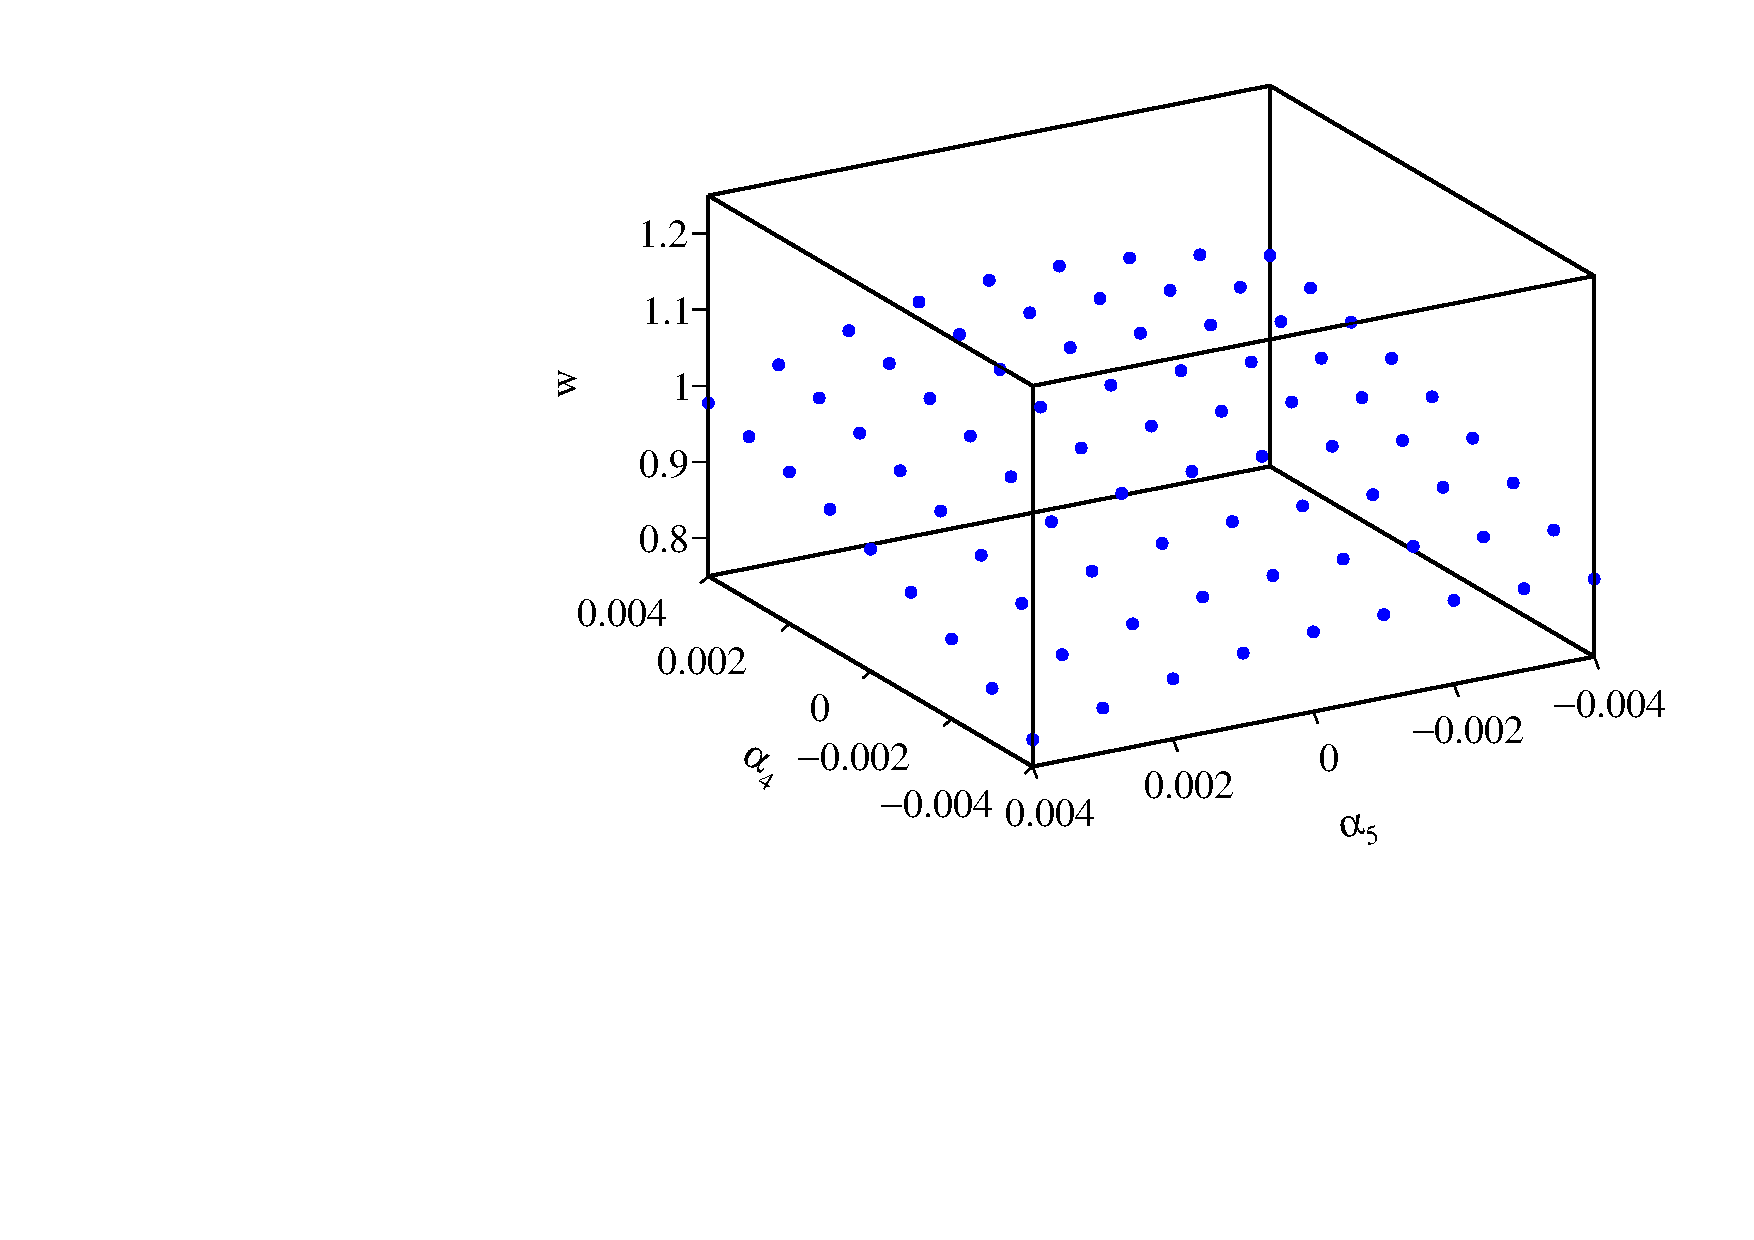
\includegraphics[width=0.5\textwidth]{PhysicsAnalysis/Plots/EventWeights/3000GeV/EventWeightsForEvent100001099_3000GeV_SPFOs_kt_0p70_10Bins_Start_0_End_10_3000GeV_Raw.pdf}}
\subfloat[]{\label{fig:weight3000GeV2}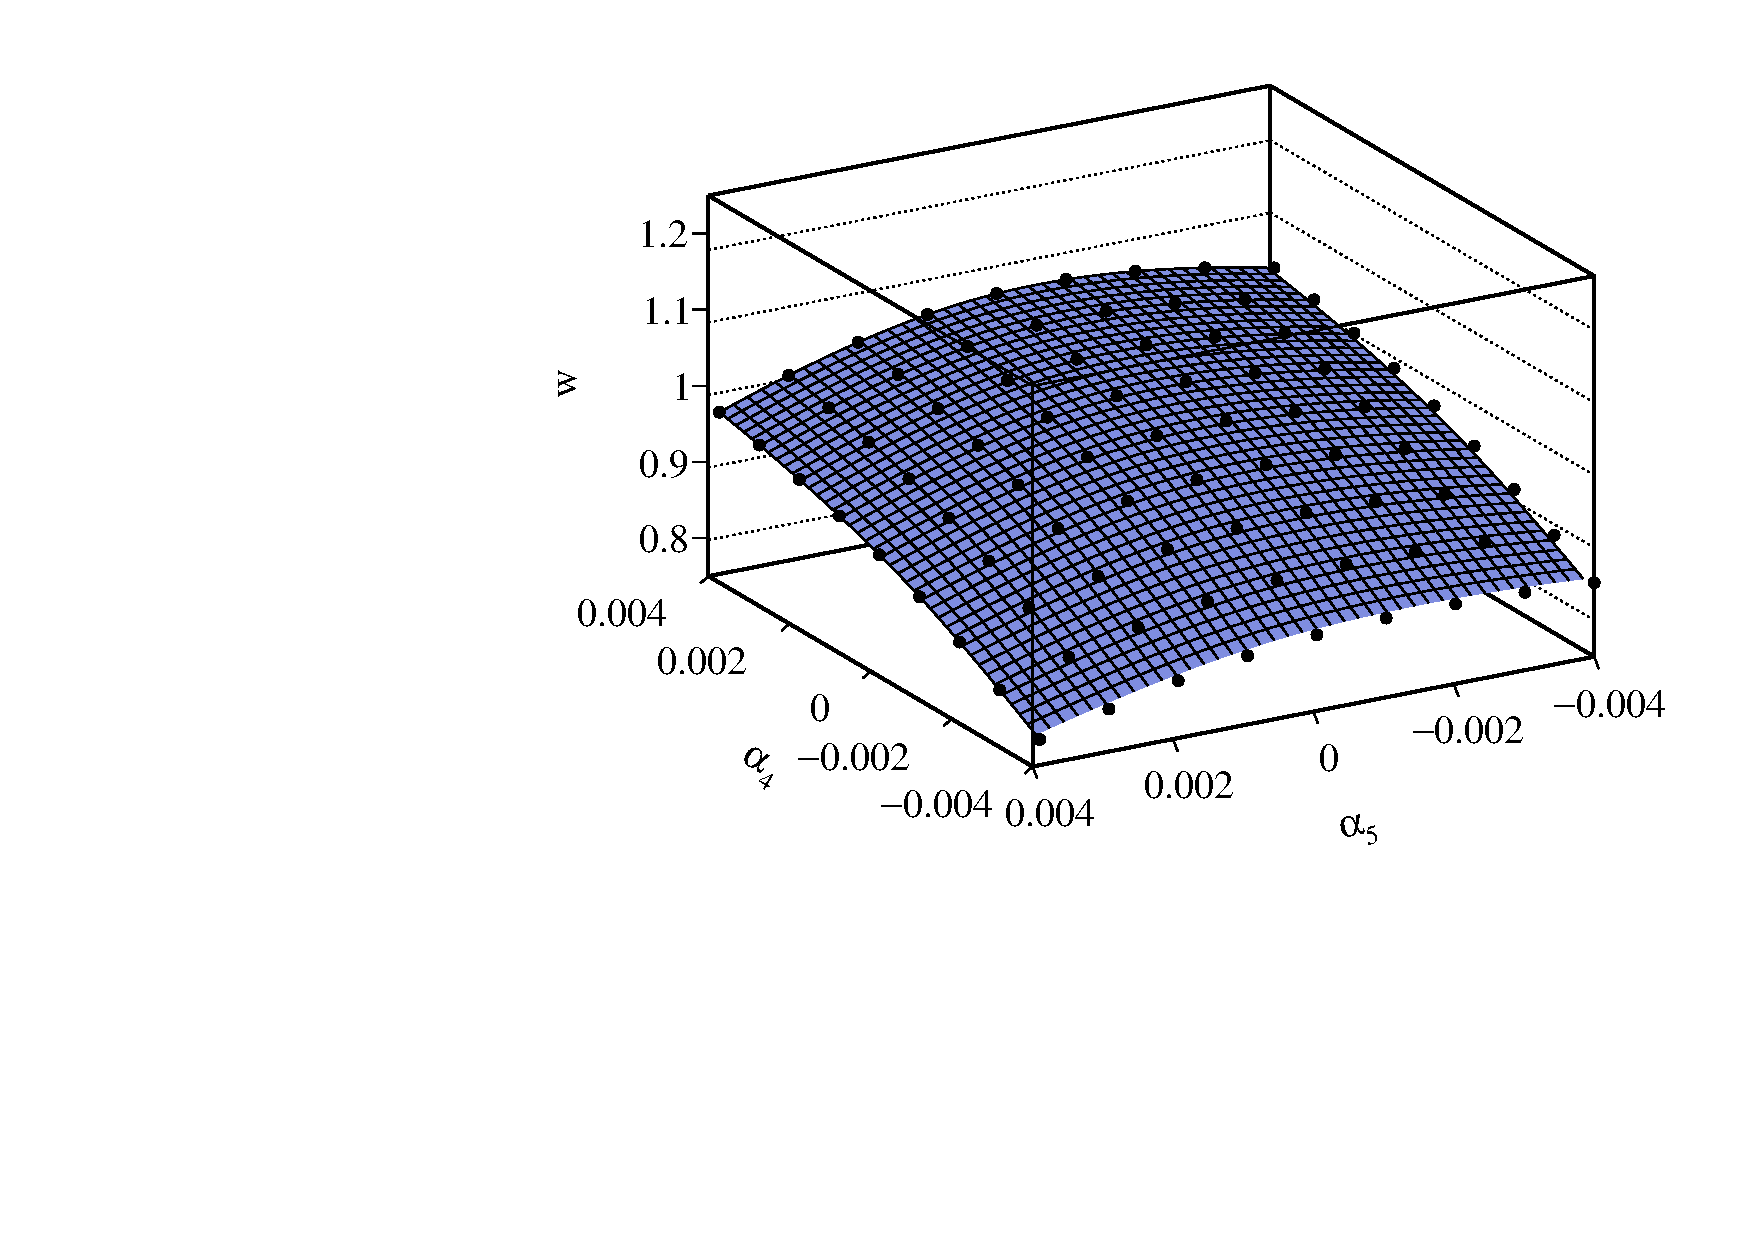
\includegraphics[width=0.5\textwidth]{PhysicsAnalysis/Plots/EventWeights/3000GeV/EventWeightsForEvent100001099_3000GeV_SPFOs_kt_0p70_10Bins_Start_0_End_10_3000GeV_Interpolated.pdf}} 
\caption[The event weights, $w$, as a function of the anomalous couplings $\alpha_{4}$ and $\alpha_{5}$ for a selected \nu{\nu}qqqq final state events at $\sqrt{s}=3$~TeV.  These weights are calculated using \protect\subref{fig:weight3000GeV1} the generator and \protect\subref{fig:weight3000GeV2} bicubic interpolation.]{The event weights, $w$, as a function of the anomalous couplings $\alpha_{4}$ and $\alpha_{5}$ for a selected \nu{\nu}qqqq final state events at $\sqrt{s}=3$~TeV.  These weights are calculated using \protect\subref{fig:weight3000GeV1} the generator and \protect\subref{fig:weight3000GeV2} bicubic interpolation.}
\label{fig:eventweights3000}
\end{figure}

A $\chi^{2}$ was applied to the distribution of $M_{VV}$ to determine the sensitivity of CLIC to the anomalous gauge couplings $\alpha_{4}$ and $\alpha_{5}$ at $\sqrt{s}=3$~TeV.  The $M_{VV}$ distribution used for the fit had an increased number of bins with respect to the $\sqrt{s}=1.4$~TeV analysis; the first bin spanned the invariant mass range between 0~GeV and 200~GeV, this was followed by 27 bins of width 100~GeV ranging from 200~GeV to 1300~GeV and finally the last bin contained all invariant masses above 2900~GeV.  Figure \ref{fig:signalbackgroundfit3000} shows the $M_{VV}$ distribution for signal and background processes at $\sqrt{s}=3$~TeV that was used in the $\chi^{2}$ fit.  

\begin{figure}[h!]
\centering
\subfloat{\label{fig:signalbackgroundfitmvv3000}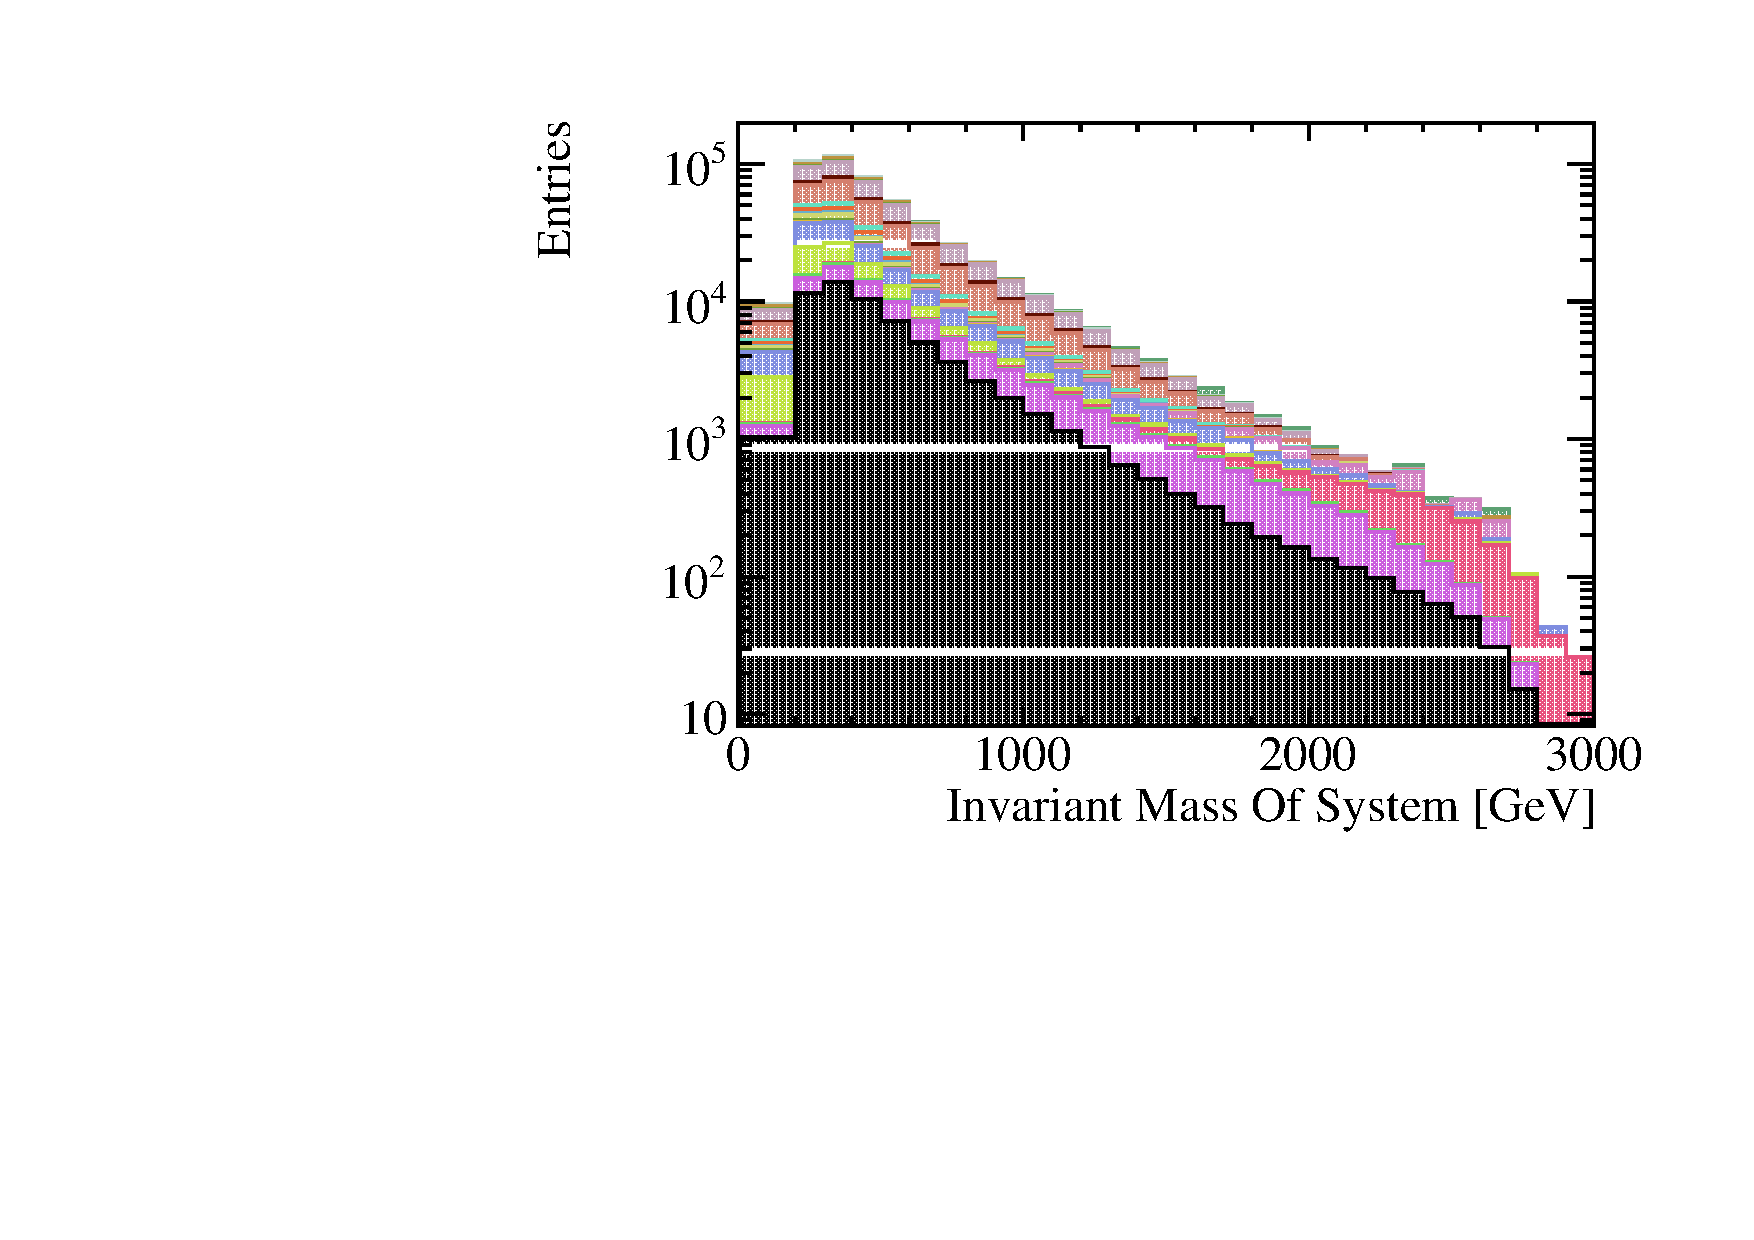
\includegraphics[width=0.5\textwidth]{PhysicsAnalysis/Plots/NuisanceFit/3000GeV/FitPlotMVV.pdf}}
\subfloat{\label{fig:signalbackgroundfitlegend3000}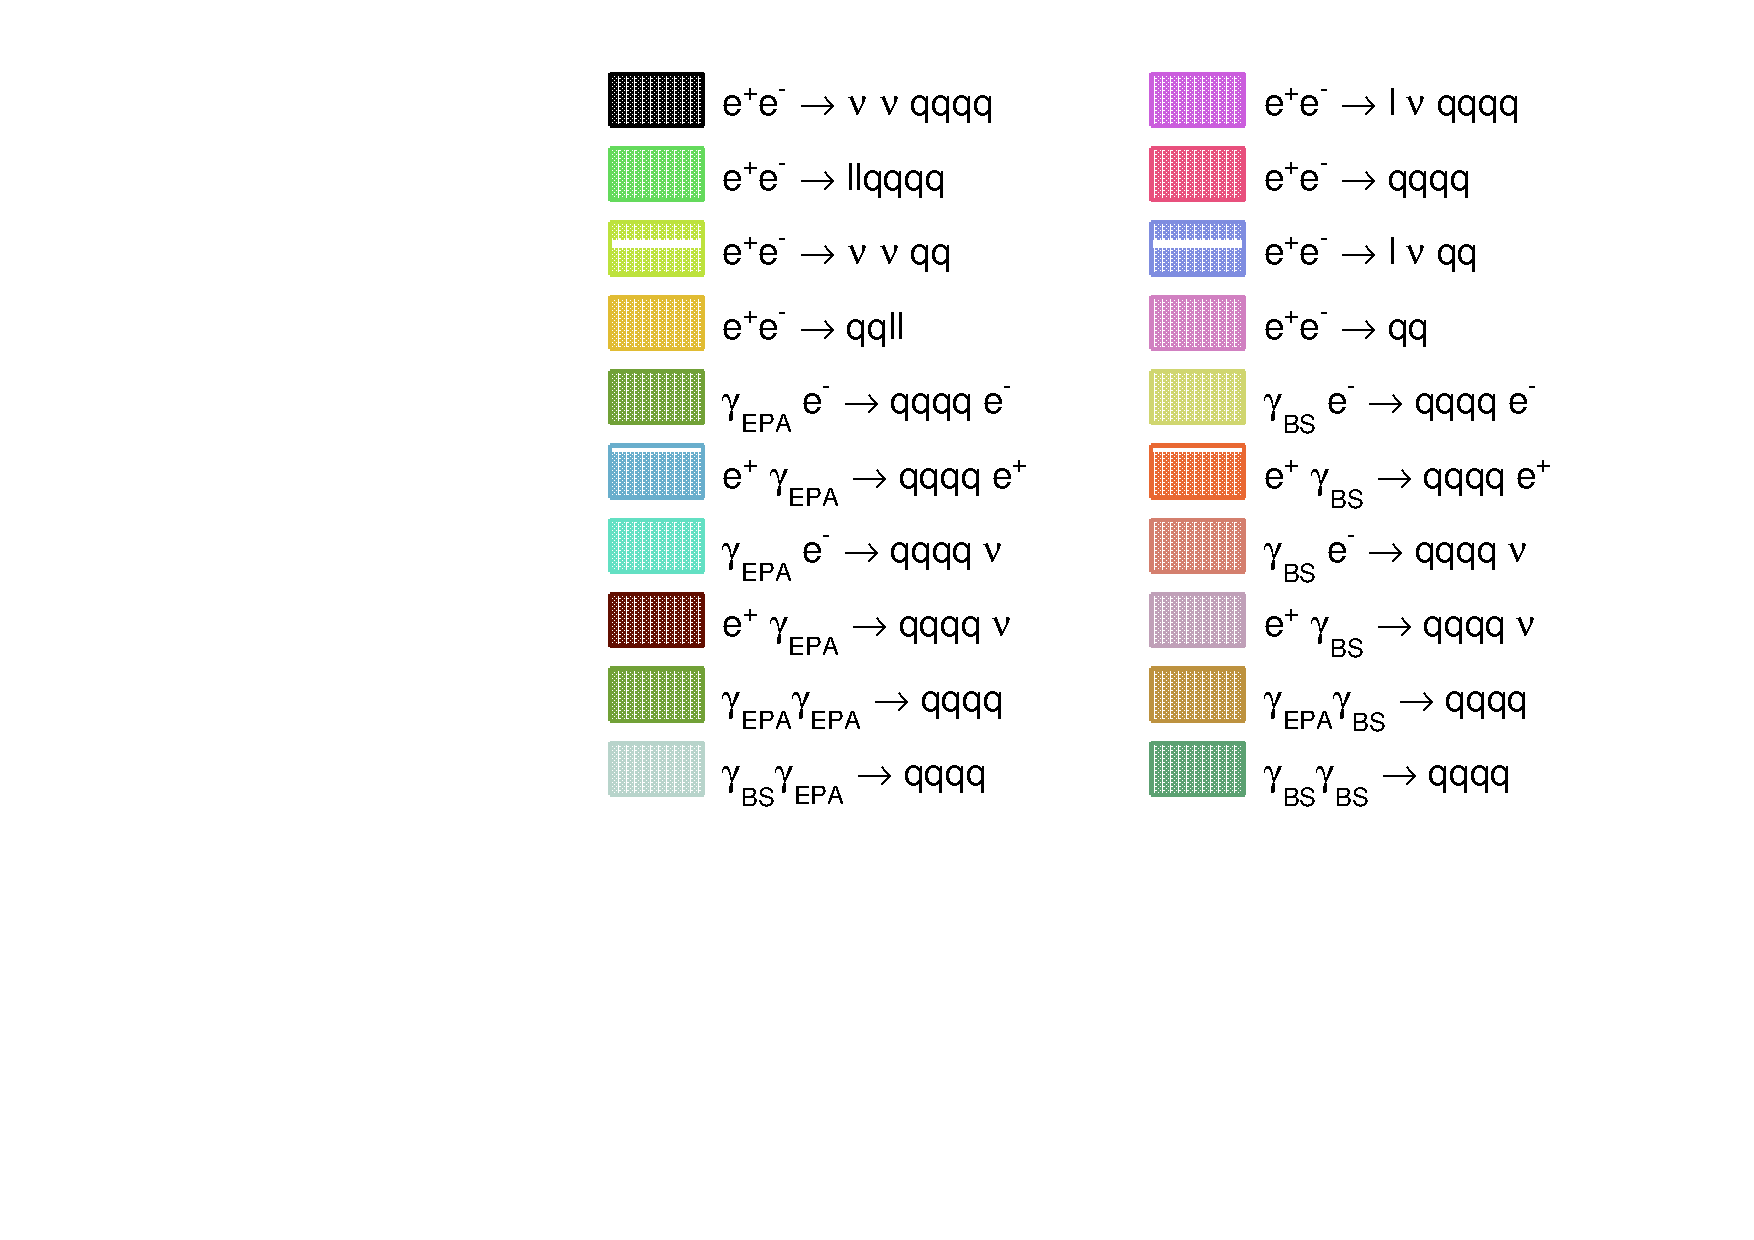
\includegraphics[width=0.5\textwidth]{PhysicsAnalysis/Plots/PreSelection/1400GeV/Legend.pdf}}
\caption[The distribution of the invariant mass of the system for both signal and background finals states that is used in the $\chi^{2}$ fit at $\sqrt{s}=3$~TeV.  The distribution includes effect of event selection and corresponds to an integrated luminosity of $\mathcal{L}_{int} = 2\text{ ab}^{-1}$.]{The distribution of the invariant mass of the system for both signal and background finals states that is used in the $\chi^{2}$ fit at $\sqrt{s}=3$~TeV.  The distribution includes effect of event selection and corresponds to an integrated luminosity of $\mathcal{L}_{int} = 2\text{ ab}^{-1}$.}
\label{fig:signalbackgroundfit3000}
\end{figure}

The sensitivity of the CLIC experiment to the anomalous gauge couplings $\alpha_{4}$ and $\alpha_{5}$ at $\sqrt{s}=3$~TeV is shown in figure \ref{fig:finalresult3000GeV}.  This result shows the sensitivity after the application of preselection and MVA, described in sections \ref{sec:preselection1400GeV} and \ref{sec:mva1400GeV}, purposed to remove the included background channels.  These contours give a 68\% confidence limit on the measurement of $\alpha_{4}$ and $\alpha_{5}$ for CLIC operating at $\sqrt{s}=3$~TeV of
%
\begin{equation}
-0.0010 < \alpha_{4} < 0.0011 \text{,} \\
-0.0007 < \alpha_{5} < 0.0007 \text{.}
\end{equation}
%

\begin{figure}[h!]
\centering
\subfloat[]{\label{fig:finalresult3000GeV}\includegraphics[width=0.5\textwidth]{PhysicsAnalysis/Plots/FinalResult/3000GeV/Final.pdf}}\hfill
\subfloat[]{\label{fig:a4finalresult3000GeV}\includegraphics[width=0.5\textwidth]{PhysicsAnalysis/Plots/FinalResult/3000GeV/Final_alpha4.pdf}}
\subfloat[]{\label{fig:a5finalresult3000GeV}\includegraphics[width=0.5\textwidth]{PhysicsAnalysis/Plots/FinalResult/3000GeV/Final_alpha5.pdf}}
\caption[$\chi^{2}$ sensitivity distributions from a fit to $M_{VV}$ at $\sqrt{s}=3$~TeV.  Results include the effect of backgrounds after the application of a series of preselection cuts and MVA.  \protect\subref{fig:finalresult3000GeV} $\chi^{2}$ sensitivity contours in $\alpha_{4}$ and $\alpha_{5}$ space.  \protect\subref{fig:a4finalresult3000GeV} $\chi^{2}$ as a function of $\alpha_{4}$ assuming $\alpha_{5} = 0$.  \protect\subref{fig:a5finalresult3000GeV} $\chi^{2}$ as a function of $\alpha_{5}$ assuming $\alpha_{4} = 0$.]{$\chi^{2}$ sensitivity distributions from a fit to $M_{VV}$ at $\sqrt{s}=3$~TeV.  Results include the effect of backgrounds after the application of a series of preselection cuts and MVA.  \protect\subref{fig:finalresult3000GeV} $\chi^{2}$ sensitivity contours in $\alpha_{4}$ and $\alpha_{5}$ space.  \protect\subref{fig:a4finalresult3000GeV} $\chi^{2}$ as a function of $\alpha_{4}$ assuming $\alpha_{5} = 0$.  \protect\subref{fig:a5finalresult3000GeV} $\chi^{2}$ as a function of $\alpha_{5}$ assuming $\alpha_{4} = 0$.}
\label{fig:allfinalresult3000GeV}
\end{figure}

Figure \ref{fig:nuisance3000GeV} shows how the 68\% confidence region for the $\sqrt{s}=3$~TeV analysis varies with the uncertainty in the cross-section for the signal, $\text{e}^{+}\text{e}^{-} \rightarrow \nu{\nu}\text{qqqq}$, and dominant background processes, $\text{e}^{\pm}\gamma_{\text{BS}} \rightarrow \nu_{\text{e}}\text{qqqq}$.  These contours were produced using a nuisance parameter as discussed in section \ref{sec:systematics}.  Once again, these systematic uncertainties have a small effect on the reported sensitivity of CLIC to the anomalous gauge couplings because of the shape of the $M_{VV}$ distribution.

\begin{figure}[h!]
\centering
\subfloat[]{\label{fig:nuisance3000GeVsig}\includegraphics[width=0.5\textwidth]{PhysicsAnalysis/Plots/NuisanceFit/3000GeV/NuisanceSignal.pdf}}\hfill
\subfloat[]{\label{fig:nuisance3000GeVbkg}\includegraphics[width=0.5\textwidth]{PhysicsAnalysis/Plots/NuisanceFit/3000GeV/Nuisance.pdf}}
\caption[The 68\% confidence region including the effect of uncertainties in the cross-section for \protect\subref{fig:nuisance3000GeVsig} the signal process $\text{e}^{+}\text{e}^{-} \rightarrow \nu{\nu}\text{qqqq}$ and \protect\subref{fig:nuisance3000GeVbkg} the dominant background processes $\text{e}^{\pm}\gamma_{\text{BS}} \rightarrow \nu_{\text{e}}\text{qqqq}$.]{The 68\% confidence region including the effect of uncertainties in the cross-section for \protect\subref{fig:nuisance3000GeVsig} the signal process $\text{e}^{+}\text{e}^{-} \rightarrow \nu{\nu}\text{qqqq}$ and \protect\subref{fig:nuisance3000GeVbkg} the dominant background processes $\text{e}^{\pm}\gamma_{\text{BS}} \rightarrow \nu_{\text{e}}\text{qqqq}$.}
\label{fig:nuisance3000GeV}
\end{figure}

%========================================================================================
%========================================================================================
